%
% Copyright 2018 Joel Feldman, Andrew Rechnitzer and Elyse Yeager.
% This work is licensed under a Creative Commons Attribution-NonCommercial-ShareAlike 4.0 International License.
% https://creativecommons.org/licenses/by-nc-sa/4.0/
%

\def\lin{{\text{LIN}}}
\def\prod{{\text{PR}}}
\def\quot{{\text{QR}}}
\def\simp{{\text{SMP}}}

\graphicspath{{figures/differentiation/}}
\chapter{Derivatives}\label{chap deriv}

Calculus is built on two operations --- differentiation, which is used to analyse
instantaneous rate of change, and integration, which is used to analyse areas.
Understanding differentiation and using it to compute derivatives of functions is one of the
main aims of this course.

We had a glimpse of derivatives in the previous chapter on limits --- in particular
Sections~\ref{sec first lim} and~\ref{sec velocity} on tangents and velocities introduced
derivatives in disguise. One of the main reasons that we teach limits is to understand
derivatives. Fortunately, as we shall see, while one does need to understand limits in
order to correctly understand derivatives, one does not need the full machinery of limits
in order to \emph{compute and work with} derivatives. The other main part of calculus,
integration, we (mostly) leave until a later course.

The derivative finds many applications in many different areas of the sciences. Indeed
the
reason that calculus is taken by so many university students is so that they may then use
the ideas both in subsequent mathematics courses and in other fields. In almost any field
in which you study quantitative data you can find calculus lurking somewhere nearby.

Its development\footnote{A quick google will turn up many articles on the development and
history of calculus. Wikipedia has a good one.} came about over a very long time,
starting
with the ancient Greek geometers. Indian, Persian and Arab mathematicians made
significant
contributions from around the $6^{\rm th}$ century. But modern calculus really starts
with
Newton and Leibniz in the $17^{\rm th}$ century who developed independently based on
ideas
of others including Descartes. Newton applied his work to many physical problems
(including orbits of moons and planets) but didn't publish his work. When Leibniz
subsequently published his ``calculus'', Newton accused him of plagiarism --- this caused
a huge rift between British and  continental-European mathematicians which wasn't closed
for another century.



%%%%%%%%%%%%%%%%%%%%%%%%%%%%%%%%%%%%%%%%%%%%%%%%%%%%%%%%%%%%%%%%%%%%%%
\section{Revisiting Tangent Lines}\label{sec_2_1}
%%%%%%%%%%%%%%%%%%%%%%%%%%%%%%%%%%%%%%%%%%%%%%%%%%%%%%%%%%%%%%%%%%%%%%


By way of motivation for the definition of the derivative, we return
to the discussion of tangent lines that we started in the previous
chapter on limits. We consider, in  Examples~\ref{eg:DIFFslopeA} and~\ref{eg:DIFFslopeB},
below, the problem of finding the slope of the tangent line to a curve at a point. But
let us start  by recalling, in Example \ref{eg:DIFFlineslope}, what is meant by the slope
of a straight line.
\begin{eg}\label{eg:DIFFlineslope}
In this example, we recall what is meant by the slope of the straight line
\begin{align*}
y&=\tfrac{1}{2}x+\tfrac{3}{2}
\end{align*}
\begin{itemize}
 \item We claim that if, as we walk along this straight line, our $x$--coordinate changes
by an amount~$\De x$, then our $y$--coordinate changes by exactly~$\De y =
\tfrac{1}{2}\De
x$.

\item For example, in the figure on the left below, we move from the point
\begin{align*}
(x_0,y_0)=(1\,,\,2=\tfrac{1}{2}\times 1+\tfrac{3}{2})
\end{align*}
on the line to the point
\begin{align*}
(x_1,y_1)=(5\,,\,4=\tfrac{1}{2}\times 5+\tfrac{3}{2})
\end{align*}
on the line. In this move our $x$--coordinate changes by
\begin{align*}
\De x= 5-1=4
\end{align*}
and our $y$--coordinate changes by
\begin{align*}
\De y=4-2=2
\end{align*}
which is indeed $\tfrac{1}{2}\times 4=\tfrac{1}{2}\De x$, as claimed.

\begin{wfig}
\begin{center}
    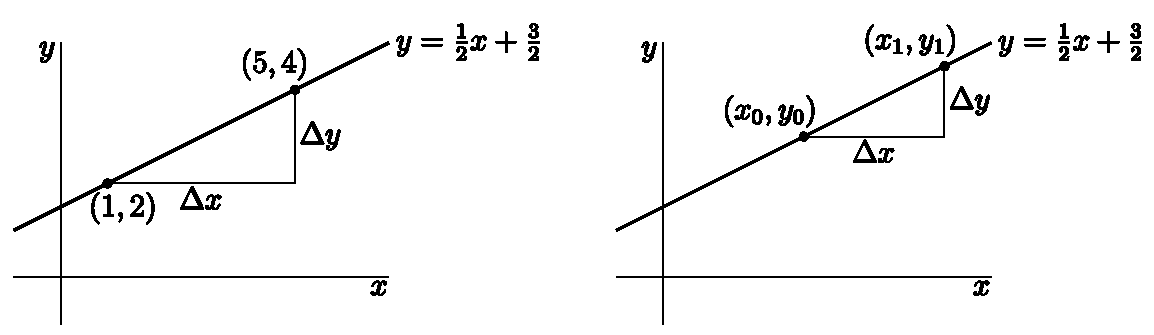
\includegraphics{slopeAB}
\end{center}
\end{wfig}

\item In general, when we move from the point
\begin{align*}
(x_0,y_0) &= (x_0, \tfrac{1}{2}x_0+\tfrac{3}{2})
\end{align*}
on the line to the point
\begin{align*}
(x_1,y_1) &= (x_1, \tfrac{1}{2}x_1+\tfrac{3}{2})
\end{align*}
on the line, our $x$--coordinate changes by
\begin{align*}
\De x=x_1-x_0
\end{align*}
and our $y$--coordinate changes by
\begin{align*}
\De y&=y_1-y_0 \\
&=\big[\tfrac{1}{2}x_1+\tfrac{3}{2}\big]
-\big[\tfrac{1}{2}x_0+\tfrac{3}{2}\big] \\
&=\tfrac{1}{2}(x_1-x_0)
\end{align*}
which is indeed $\tfrac{1}{2}\De x$, as claimed.

\item So, for the straight line $y=\tfrac{1}{2}x+\tfrac{3}{2}$, the ratio $\tfrac{\De
y}{\De x} =\tfrac{y_1-y_0}{x_1-x_0}$ always takes the value $\frac{1}{2}$,
regardless of the choice of initial point $(x_0,y_0)$ and final point
$(x_1,y_1)$. This constant ratio is the slope of the line $y=\tfrac{1}{2}x+\tfrac{3}{2}$.
\end{itemize}
\end{eg}

Straight lines are special in that for each straight line, there is a fixed number
$m$, called the slope of the straight line, with the property that if you
take \emph{any} two different points, $(x_0,y_0)$ and $(x_1,y_1)$, on the line,
the ratio  $\tfrac{\De y}{\De x}=\tfrac{y_1-y_0}{x_1-x_0}$,
which is called the rate of change of $y$ per unit rate of
change\footnote{In the ``real world'' the phrase ``rate of change'' usually
refers to rate of change per unit time. In science it used more generally.}
of $x$, always takes the value $m$. This is the property that distinguishes
lines from other curves.

Other curves do not have this property. In the next two examples we illustrate this
point with the parabola $y=x^2$. Recall that we studied this example back in
Section~\ref{sec first lim}. In Example~\ref{eg:DIFFslopeA} we find the slope of the
tangent line to $y=x^2$ at a particular point. We generalise this in Example
\ref{eg:DIFFslopeB}, to show that we can define ``the slope of the curve $y=x^2$'' at an
arbitrary point $x=x_0$ by  considering $\tfrac{\De y}{\De x}=\tfrac{y_1-y_0}{x_1-x_0}$
with $(x_1,y_1)$ very close to $(x_0,y_0)$.


\begin{eg}\label{eg:DIFFslopeA}
In this example, let us fix $(x_0,y_0)$ to be the point $(2,4)$
on the parabola $y=x^2$. Now let $(x_1, y_1) = (x_1, x_1^2)$ be some other
point on the parabola; that is, a point with $x_1 \neq x_0$.

\begin{itemize}
\item Draw the straight line through $(x_0,y_0)$ and $(x_1,y_1)$ --- this is a secant
line and we saw these in Chapter~\ref{chap limits} when we discussed tangent
lines\footnote{If you do not remember this, then please revisit the first couple of
sections of Chapter~\ref{chap limits}.}.

\item The following table gives the slope, $\tfrac{y_1-y_0}{x_1-x_0}$, of the secant line
through $(x_0,y_0)=(2,4)$ and $(x_1,y_1)$, for various different choices of
$(x_1,y_1=x_1^2)$.

\renewcommand{\arraystretch}{1.3}
\begin{center}
     \begin{tabular}{|c||c|c|c|c|c|c|c|c|c|c|c|}
          \hline
          $x_1$ &
              $1$ & $1.5$ & $1.9$ & $1.99$ & $1.999$ & $\circ$
                                & $2.001$ & $2.01$
                                & $2.1$ & $2.5$ & $3$ \\ \hline
          $y_1=x_1^2$ &
             $1$ & $2.25$ & $3.61$ & $3.9601$ & $3.9960$ & $\circ$
                                & $4.0040$ & $4.0401$
                                & $4.41$ & $6.25$ & $9$ \\ \hline
          $\tfrac{y_1-y_0}{x_1-x_0}=\tfrac{y_1-4}{x_1-2}\!$ &
              $3$ & $3.5$ & $3.9$ & $3.99$ & $3.999$ & $\circ$
                                & $4.001$ & $4.01$
                                & $4.1$ & $4.5$ & $5$ \\ \hline
     \end{tabular}
\end{center}
% \begin{center}
%      \begin{tabular}{|c||c|c|c|c|c|c||c|c|c|c|c|c|}
%           \hline
%           $x_1$ &
%               $0$ & $1$ & $1.5$ & $1.9$ & $1.99$ & $1.999$
%                                 & $2.001$ & $2.01$
%                                 & $2.1$ & $2.5$ & $3$ & $4$\\ \hline
%           $y_1=x_1^2$ &
%              $0$ & $1$ & $2.25$ & $3.61$ & $3.9601$ & $3.9960$
%                                 & $4.0040$ & $4.0401$
%                                 & $4.41$ & $6.25$ & $9$ & $16$\\ \hline
%           $\tfrac{y_1-y_0}{x_1-x_0}=\tfrac{y_1-4}{x_1-2}\!$ &
%               $2$ & $3$ & $3.5$ & $3.9$ & $3.99$ & $3.999$
%                                 & $4.001$ & $4.01$
%                                 & $4.1$ & $4.5$ & $5$ & $6$\\ \hline
%      \end{tabular}
% \end{center}
\renewcommand{\arraystretch}{1.0}

\item So now we have a big table of numbers --- what do we do with them?
Well, there are messages we can take away from this table.
\begin{itemize}
\item
   Different choices of $x_1$ give different values for the
   slope, $\tfrac{y_1-y_0}{x_1-x_0}$, of the secant through
   $(x_0,y_0)$ and $(x_1,y_1)$. This is illustrated in Figure
   \ref{fig:multislope} below
   --- the slope of the secant through $(x_0,y_0)$ and $(x_1,y_1)$ is different from the
slope of the secant through $(x_0,y_0)$ and $(x'_1,y'_1)$.

  \begin{sfig}
  \label{fig:multislope}
  \begin{center}
  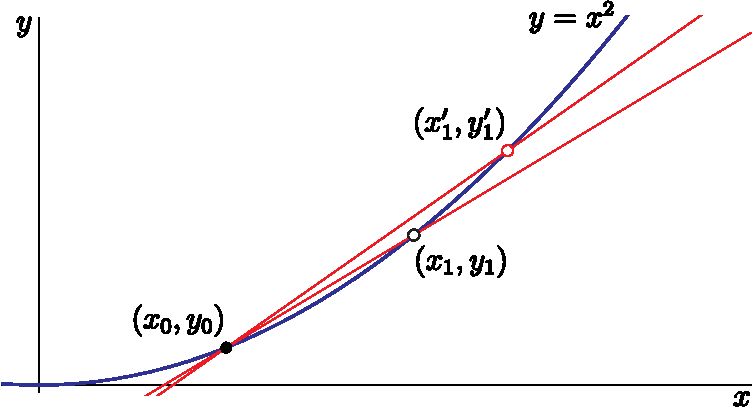
\includegraphics{slopeD}

   For a curvy curve, different secants have different slopes.
  \end{center}
  \end{sfig}

   If the parabola were a straight
   line this would not be the case  --- the secant through any two different
   points on a line is always identical to the line itself and so always
   has exactly the same slope as the line itself, as is illustrated in
   Figure \ref{fig:singleslope} below --- the (yellow) secant through
   $(x_0,y_0)$ and $(x_1,y_1)$ lies exactly on top of the (red)
   line $y=\tfrac{1}{2}x+\tfrac{3}{2}$.
   \issue{Colours in\\ fig will not\\ work when\\ printed in\\ black and\\
   white.}


 \begin{sfig}
 \label{fig:singleslope}
 \begin{center}
 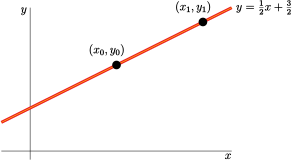
\includegraphics{slopeE}

 For a straight line, all secants have the same slope.
 \end{center}
 \end{sfig}

\item Now look at the columns of the table closer to the middle. As $x_1$ gets closer
and closer to $x_0=2$, the slope, $\tfrac{y_1-y_0}{x_1-x_0}$, of the secant through
   $(x_0,y_0)$ and $(x_1,y_1)$ appears to get closer and closer to the
   value $4$.
\end{itemize}
\end{itemize}
\end{eg}

\begin{eg}\label{eg:DIFFslopeB}
 It is very easy to generalise what is happening in Example \ref{eg:DIFFslopeA}.
\begin{itemize}
 \item Fix any point $(x_0,y_0)$ on the parabola $y=x^2$. If $(x_1,y_1)$ is any other
point on the parabola $y=x^2$, then $y_1=x_1^2$ and the slope of the secant through
$(x_0,y_0)$ and $(x_1,y_1)$ is
\begin{align*}
   \text{slope}
   &= \frac{y_1-y_0}{x_1-x_0}
    =\frac{x_1^2-x_0^2}{x_1-x_0} && \text{since $y=x^2$} \\
  & =\frac{(x_1-x_0)(x_1+x_0)}{x_1-x_0} && \text{remember $a^2-b^2 =
(a-b)(a+b)$}  \\
  & =x_1+x_0
\end{align*}
You should check the values given in the table of Example \ref{eg:DIFFslopeA}
above to convince yourself that the slope $\tfrac{y_1-y_0}{x_1-x_0}$
of the secant line really is $x_0+x_1 = 2+x_1$ (since we set
$x_0=2)$.

\item Now as we move $x_1$ closer and closer to $x_0$, the slope should move
closer and closer to $2x_0$. Indeed if we compute the limit carefully --- we
now have the technology to do this --- we see that in the limit as
$x_1 \to x_0$ the slope becomes $2x_0$.
That is
\begin{align*}
  \lim_{x_1 \to x_0} \frac{y_1-y_0}{x_1-x_0}
  &= \lim_{x_1 \to x_0} (x_1+x_0) \qquad \text{by the work we did just above} \\
  &= 2x_0
\end{align*}
Taking this limit gives us our first derivative. Of course we haven't yet
given the definition of a derivative, so we perhaps wouldn't recognise it yet.
We rectify this in the next section.

\begin{sfig}
   \label{fig:secantToTangent}
   \begin{center}
   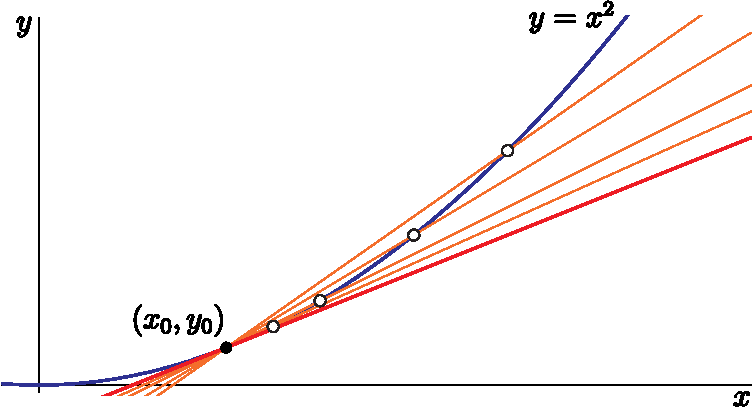
\includegraphics{slopeC}

   Secants approaching a tangent line
  \end{center}
\end{sfig}

\noindent
\item So it is reasonable to say ``as $x_1$ approaches $x_0$, the secant through
$(x_0,y_0)$ and $(x_1,y_1)$ approaches the tangent line to the parabola $y=x^2$ at
$(x_0,y_0)$''. This is what we did back in Section~\ref{sec first lim}.

The figure above shows four different secants through $(x_0,y_0)$ for the curve $y=x^2$.
The four hollow circles are four different choices of $(x_1,y_1)$. As $(x_1,y_1)$
approaches $(x_0,y_0)$, the corresponding secant does indeed approach the tangent to
$y=x^2$ at $(x_0,y_0)$, which is the heavy (red) straight line in the figure.

Using limits we determined the slope of the tangent line to $y=x^2$ at $x_0$ to be
$2x_0$. Often we will be a little sloppy with our language and instead say ``the
slope of the parabola $y=x^2$ at $(x_0,y_0)$ is $2x_0$'' --- where we really mean the
slope of the line tangent to the parabola at $x_0$.



\end{itemize}
\end{eg}

%%%%%%%%%%%%%%%%%%%%%%%%%%%%%%%%%%%%%%%%%%%%%%%%%%%%%%%%%%%%%%%%%%%%%%
\section{Definition of the Derivative} \label{sec def deriv}
%%%%%%%%%%%%%%%%%%%%%%%%%%%%%%%%%%%%%%%%%%%%%%%%%%%%%%%%%%%%%%%%%%%%%%
We now define the ``derivative'' explicitly, based on the limiting
slope ideas of the previous section. Then we see how to compute some simple
derivatives.

Let us now generalise what we did in the last section so as
to find ``the slope of the curve $y=f(x)$ at $(x_0,y_0)$''
for any smooth enough\footnote{The idea of ``smooth enough'' can be made
quite precise. Indeed the word ``smooth'' has a very precise
meaning in mathematics, which we won't cover here. For now think of
``smooth'' as meaning roughly just ``smooth''.} function $f(x)$.

As before, let $(x_0,y_0)$ be any point on the curve $y=f(x)$.
So we must have $y_0=f(x_0)$. Now let $(x_1,y_1)$ be any other point
on the same curve. So $y_1=f(x_1)$ and $x_1\ne x_0$.  Think of $(x_1,y_1)$
as being pretty close to $(x_0,y_0)$ so that the difference
\begin{align*}
\De x=x_1-x_0
\end{align*}
in $x$--coordinates is pretty small. In terms of this  $\De x$ we have
\begin{align*}
x_1=x_0+\De x\qquad\text{and}\qquad
y_1=f\big(x_0+\De x\big)
\end{align*}
We can construct a secant line through $(x_0,y_0)$ and $(x_1,y_1)$ just
as we did for the parabola above. It has slope
\begin{align*}
\frac{y_1-y_0}{x_1-x_0}=\frac{f\big(x_0+\De x\big)-f(x_0)}{\De x}
\end{align*}
If $f(x)$ is reasonably smooth\footnote{Again the term ``reasonably smooth'' can be made
more precise.}, then as $x_1$ approaches $x_0$, i.e. as $\De x$ approaches $0$,
we would expect the secant through $(x_0,y_0)$ and $(x_1,y_1)$ to approach the
tangent line to the curve $y=f(x)$ at $(x_0,y_0)$, just as happened in Figure
\ref{fig:secantToTangent}. And more importantly, the slope of the secant through
$(x_0,y_0)$ and $(x_1,y_1)$ should approach the slope of the tangent line to the
curve  $y=f(x)$ at $(x_0,y_0)$.

Thus we would expect\footnote{Indeed, we don't have to expect --- it is!}
the slope of the tangent line to the curve  $y=f(x)$ at $(x_0,y_0)$ to be
\begin{align*}
\lim_{\De x\rightarrow 0}\frac{f\big(x_0+\De x\big)-f(x_0)}{\De x}
\end{align*}
When we talk of the ``slope of the curve'' at a point, what we really
mean is the slope of the tangent line to the curve at that point. So
``the slope of the curve  $y=f(x)$ at $(x_0,y_0)$'' is also the
limit\footnote{This is of course under the assumption that
the limit exists --- we will talk more about that below.}
expressed in the above equation. The derivative of $f(x)$ at $x=x_0$ is also defined
to be this limit. Which leads\footnote{We will rename ``$x_0$'' to ``$a$'' and ``$\De
x$''
to ``$h$''.} us to the most important definition in this text:

\begin{defn}[Derivative at a point]\label{def:DIFFderiv}
Let $a\in\bbbr$ and let $f(x)$ be defined on an open interval\footnote{
  Recall, from Definition~\ref{def intervals}, that the open interval $(c,d)$ is
  just the set of all real numbers obeying $c<x<d$.}
that contains $a$.
\begin{itemize}
 \item The derivative of $f(x)$ at $x=a$ is denoted
$f'(a)$ and is defined by
\begin{align*}
f'(a)=\lim_{h\rightarrow 0}\frac{f\big(a+h\big)-f(a)}{h}
\end{align*}
if the limit exists.
\item When the above limit exists, the function $f(x)$ is said
to be differentiable at $x=a$. When the limit does not  exist, the
function $f(x)$ is said to be not differentiable at $x=a$.

\item We can equivalently define the derivative $f'(a)$ by the limit
\begin{align*}
f'(a)=\lim_{x\rightarrow a}\frac{f(x)-f(a)}{x-a}.
\end{align*}
To see that these two definitions are the same, we set $x=a+h$ and then the limit as
$h$ goes to $0$ is equivalent to the limit as $x$ goes to $a$.
\end{itemize}
\end{defn}


Lets now compute the derivatives of some very simple functions. This is our first step
towards building up a toolbox for computing derivatives of complicated functions ---
this process will very much parallel what we did in Chapter~\ref{chap limits} with
limits. The two simplest functions we know are $f(x)=c$ and $g(x)=x$.
\begin{eg}[Derivative of $f(x)=c$]\label{eg:DIFFderivX0}
Let $a, c \in \bbbr$ be a constants. Compute the derivative of the constant function
$f(x) = c$ at $x=a$.

We compute the desired derivative by just substituting the function
of interest into the formal definition of the derivative.
\begin{align*}
  f'(a) &= \lim_{h \to 0} \frac{f(a+h) - f(a)}{h} && \text{(the definition)}\\
  &= \lim_{h \to 0} \frac{c - c}{h} && \text{(substituted in the function)} \\
  &= \lim_{h \to 0} 0 &&\text{(simplified things)}\\
  &= 0
\end{align*}
\end{eg}
That was easy! What about the next most complicated function ---
arguably it's this one:

\begin{eg}[Derivative of $g(x)=x$]\label{eg:DIFFderivX1}
Let $a\in \bbbr$ and compute the derivative of $g(x) = x$ at $x=a$.

Again, we compute the derivative of $g$ by just substituting the function
of interest into the formal definition of the derivative and then evaluating
the resulting limit.
\begin{align*}
  g'(a) &= \lim_{h \to 0} \frac{g(a+h) - g(a)}{h}
                  && \text{(the definition)}\\
  &= \lim_{h \to 0} \frac{(a+h) - a}{h}
                   && \text{(substituted in the function)} \\
  &= \lim_{h \to 0} \frac{h}{h} && \text{(simplified things)} \\
  &= \lim_{h \to 0} 1 && \text{(simplified a bit more)}\\
  &= 1
\end{align*}

\end{eg}

That was a little harder than the first example, but still quite straight forward ---
start with the definition and apply what we know about limits.

Thanks to these two examples, we have our first theorem about derivatives:
\begin{theorem}[Easiest derivatives]\label{thm:DIFFbasicderivs}
  Let $a,c \in \mathbb{R}$ and let $f(x) = c$ be the constant function and
$g(x) = x$. Then
\begin{align*}
  f'(a) &= 0
\intertext{and }
  g'(a) &= 1.
\end{align*}
\end{theorem}

To ratchet up the difficulty a little bit more, let us redo the example we have already
done a few times $f(x)=x^2$. To make it a little more interesting let's change the names
of the function and the variable so that it is not exactly the same as Examples~
\ref{eg:DIFFslopeA} and~\ref{eg:DIFFslopeB}.
\begin{eg}[Derivative of $h(t)=t^2$]\label{eg:DIFFderivX2}
Compute the derivative of
\begin{align*}
  h(t) &= t^2 & \text{ at $t=a$}
\end{align*}

\begin{itemize}
 \item This function isn't quite like the ones we saw earlier ---  it's
a function of $t$ rather than $x$. Recall that a function is a rule
which assigns to each input value an output value. So far, we have
usually called the input value $x$. But this ``$x$'' is just a dummy variable
representing a generic input value. There is nothing wrong with calling
a generic input value $t$ instead. Indeed, from time to time you will
see functions that are not written as formulas involving $x$, but instead
are written as formulas in  $t$ (for example representing
time --- see Section~\ref{sec velocity}), or $z$ (for example
representing height), or other symbols.

\item So let us write the definition of the derivative
\begin{align*}
  f'(a) &= \lim_{h \to 0} \frac{f(a+h)-f(a)}{h}
\end{align*}
and then translate it to the function names and variables at hand:
\begin{align*}
  h'(a) &= \lim_{h \to 0} \frac{h(a+h)-h(a)}{h}
\end{align*}
\item But there is a problem --- ``$h$'' plays two roles here --- it is both
the function name and the small quantity that is going to zero in our limit.
It is extremely dangerous to have a symbol represent two different things
in a single computation. We need to change one of them. So let's rename
the small quantity that is going to zero in our limit from ``$h$'' to
``$\De t$'':
\begin{align*}
  h'(a) &= \lim_{\De t \to 0} \frac{h(a+\De t)-h(a)}{\De t}
\end{align*}
\item Now we are ready to begin. Substituting in what the function $h$ is,
\begin{align*}
 h'(a) &= \lim_{\De t \to 0} \frac{(a+\De t)^2-a^2}{\De t}  \\
  &= \lim_{\De t \to 0} \frac{a^2+2a\,\De t+\De t^2-a^2}{\De t}
           && \big(\text{just squared out $(a+\De t)^2$}\big) \\
  &= \lim_{\De t \to 0} \frac{2a\,\De t+\De t^2}{\De t}  \\
  &= \lim_{\De t \to 0} (2a +\De t)  \\
  &= 2a
\end{align*}
\item You should go back check that this is what we got in Example
\ref{eg:DIFFslopeB} --- just some names have been changed.

\end{itemize}

\end{eg}

\subsection*{An Important Point (and Some Notation)}

Notice here that the answer we get depends on our choice of $a$ --- if we want to know
the derivative at $a=3$ we can just substitute $a=3$ into our answer $2a$ to get the
slope is 6. If we want to know at $a=1$ (like at the end of Section~\ref{sec first
lim}) we substitute $a=1$ and get the slope is 2. The important thing here is that we can
move from the derivative being computed at a specific point to the derivative
being a function itself --- input any value of $a$ and it returns the slope of
the tangent line to the curve at the point $x=a$, $y=h(a)$. The variable $a$ is a
dummy variable. We can rename $a$ to anything we want, like $x$, for example. So
we can replace every $a$ in
\begin{align*}
  h'(a)&=2a &\text{ by $x$, giving} && h'(x) &=2x
\end{align*}
where all we have done is replaced the symbol $a$ by the symbol $x$.

We can do this more generally and tweak the derivative at a specific point $a$ to
obtain the derivative as a function of $x$. We replace
\begin{align*}
  f'(a) &= \lim_{h \to 0} \frac{f(a+h)-f(a)}{h}
\intertext{with}
  f'(x) &= \lim_{h \to 0} \frac{f(x+h)-f(x)}{h}
\end{align*}
which gives us the following definition
\begin{defn}[Derivative as a function]\label{def:DIFFderivFunc}
Let $f(x)$ be a function.
\begin{itemize}
\item The derivative of $f(x)$ with respect to $x$ is
\begin{align*}
f'(x)=\lim_{h\rightarrow 0}\frac{f\big(x+h\big)-f(x)}{h}
\end{align*}
provided the limit exists.

 \item If the derivative $f'(x)$ exists for all $x \in (a,b)$ we say that $f$ is
differentiable on $(a,b)$.

\item Note that we will sometimes be a little sloppy with our discussions and
simply write ``$f$ is differentiable'' to mean ``$f$ is differentiable on an interval we
are interested in'' or ``$f$ is differentiable everywhere''.
\end{itemize}

\end{defn}
Notice that we are no longer thinking of tangent lines, rather this is an operation we
can do on a function. For example:

\begin{eg}[The derivative of $f(x)=\tfrac{1}{x}$]\label{eg:DIFFderivXm1}
Let $f(x) = \frac{1}{x}$ and compute its derivative with respect to $x$ --- think
carefully about where the derivative exists.
\begin{itemize}
 \item Our first step is to write down the definition of the derivative --- at
this stage, we know of no other strategy for computing derivatives.
\begin{align*}
f'(x)&=\lim_{h\rightarrow 0}\frac{f(x+h)-f(x)}{h}
     && \text{(the definition)}
\end{align*}
\item And now we substitute in the function and compute the limit.
\begin{align*}
f'(x)&=\lim_{h\rightarrow 0}\frac{f(x+h)-f(x)}{h}
     && \text{(the definition)} \\
&=\lim_{h\rightarrow 0}\frac{1}{h}\left[\frac{1}{x+h}-\frac{1}{x}\right]
     && \text{(substituted in the function)} \\
&=\lim_{h\rightarrow 0}\frac{1}{h}\ \frac{x-(x+h)}{x(x+h)}
     && \text{(wrote over a common denominator)} \\
&=\lim_{h\rightarrow 0}\frac{1}{h}\ \frac{-h}{x(x+h)}
     && \text{(started cleanup)} \\
&=\lim_{h\rightarrow 0} \frac{-1}{x(x+h)} \\
&=-\frac{1}{x^2}
\end{align*}
\item Notice that the original function $f(x)=\frac{1}{x}$ was not defined at
$x=0$ and  the derivative is also not defined  at $x=0$. This does happen more
generally --- if $f(x)$ is not defined at a particular point $x=a$, then the derivative
will not exist at that point either.
\end{itemize}

\end{eg}




So we now have two slightly different ideas of derivatives:
\begin{itemize}
 \item The derivative $f'(a)$ at a specific point $x=a$, being the slope of the tangent
line to the curve at $x=a$, and
\item The derivative as a function, $f'(x)$ as defined in
Definition~\ref{def:DIFFderivFunc}.
\end{itemize}
Of course, if we have $f'(x)$ then we can always recover the derivative at a specific
point by substituting $x=a$.


As we noted at the beginning of the chapter, the derivative was discovered independently
by Newton and Leibniz in the late $17^{\rm th}$ century. Because their discoveries were
independent, Newton and Leibniz did not have exactly the same notation. Stemming from
this, and from the many different contexts in which derivatives are used, there are quite
a few alternate notations for the derivative:

\begin{notn}\label{notn higher diff}
The following notations are all used for ``the derivative of $f(x)$ with respect to $x$''
\begin{align*}
f'(x) \qquad
\diff{f}{x} \qquad
\diff{}{x}f(x) \qquad
\dot f(x) \qquad
Df(x) \qquad
D_x f(x),
\end{align*}
while the following notations are all used for ``the derivative of $f(x)$ at $x=a$''
\begin{align*}
f'(a) \qquad
\diff{f}{x}(a) \qquad
\diff{}{x}f(x)\,\bigg|_{x=a} \qquad
\dot f(a) \qquad
Df(a) \qquad
D_x f(a).
\end{align*}


Some things to note about these notations:
\begin{itemize}
 \item We will generally use the first three, but you should recognise
them all. The notation $f'(a)$ is due to Lagrange, while the notation
$\diff{f}{x}(a)$ is due to Leibniz. They are both very useful. Neither
can be considered ``better''.

\item Leibniz notation writes the derivative as a ``fraction'' --- however it
is definitely not a fraction and should not be thought of in that way. It is
just shorthand, which is read as ``the derivative of $f$ with respect to
$x$''.

\item You read $f'(x)$ as ``$f$--prime of $x$'', and $\diff{f}{x}$ as
``dee--$f$--dee--$x$'', and $\diff{ }{x}f(x)$ as ``dee-by--dee--$x$ of $f$''.

\item Similarly you read $\diff{f}{x}(a)$ as ``dee--$f$--dee--$x$ at $a$'',
and $\diff{ }{x}f(x)\Big|_{x=a}$ as ``dee-by-dee $x$ of $f$ at $x$ equals $a$''.

\item The notation $\dot f$ is due to Newton. In physics, it is common
to use $\dot f(t)$ to denote the derivative of $f$ with respect to time.
\end{itemize}

\end{notn}


\subsection*{Back to Computing Some Derivatives}



At this point we could try to start working out how derivatives interact with
arithmetic and make an ``Arithmetic of derivatives'' theorem just like the one
we saw for limits (Theorem 2\issue{Need ref \\label}). We will get there
shortly, but before that it is important that we become more comfortable with
computing derivatives using limits and then understanding what the derivative actually
means. So --- more examples.

\begin{eg}[$\diff{}{x}\sqrt{x}$]\label{eg:DIFFderivXsqrt}
Compute the derivative, $f'(a)$, of the function $f(x)=\sqrt{x}$ at the point
$x=a$ for any $a> 0$.

\begin{itemize}
 \item So again we start with the definition of derivative and go from there:
\begin{align*}
f'(a)
&=\lim_{x\rightarrow a}\frac{f(x)-f(a)}{x-a}
 =\lim_{x\rightarrow a}\frac{\sqrt{x}-\sqrt{a}}{x-a}
\end{align*}
\item As $x$ tends to $a$, the numerator and denominator both tend to zero.
But $\tfrac{0}{0}$ is not defined. So to get a well defined limit we need
to exhibit a cancellation between the numerator and denominator ---
just as we saw in Examples~\ref{eg zero cancel limit} and~\ref{eg zero cancel limit
harder}. Now there are two equivalent ways to proceed from here, both based on a similar
``trick''.

\item For the first, review Example~\ref{eg zero cancel limit
harder}, which concerned taking a limit involving square-roots, and recall that
we used  ``multiplication by the conjugate'' there:
\begin{align*}
  \frac{\sqrt{x}-\sqrt{a}}{x-a}
  &= \frac{\sqrt{x}-\sqrt{a}}{x-a} \times
              \frac{\sqrt{x}+\sqrt{a}}{\sqrt{x}+\sqrt{a}}
  && \Big(\text{multiplication by
        $1=\frac{\text{conjugate}}{\text{conjugate}}$}\Big)\\
  &=\frac{(\sqrt{x}-\sqrt{a})(\sqrt{x}+\sqrt{a})}
                        {(x-a)(\sqrt{x}+\sqrt{a})} \\
  &= \frac{x-a}{(x-a)(\sqrt{x}+\sqrt{a})}
  && \big(\text{since $(A-B)(A+B) = A^2-B^2$)}\,\big) \\
  &= \frac{1}{\sqrt{x}+\sqrt{a}}
\end{align*}
\item Alternatively, we can arrive at
$\frac{\sqrt{x}-\sqrt{a}}{x-a}=\frac{1}{\sqrt{x}+\sqrt{a}}$
by using almost the same trick to factor the denominator.
Just set $A=\sqrt{x}$ and  $B=\sqrt{a}$ in
$
  A^2 - B^2 = (A-B)(A+B)
$
to get
\begin{align*}
  x - a &= (\sqrt{x}-\sqrt{a})(\sqrt{x}+\sqrt{a})
\end{align*}
and then substitute this little fact into our expression
\begin{align*}
  \frac{\sqrt{x}-\sqrt{a}}{x-a}
  &=\frac{\sqrt{x}-\sqrt{a}}{(\sqrt{x}-\sqrt{a})(\sqrt{x}+\sqrt{a})}
  & \text{(now cancel common factors)}\\
  &=\frac{1}{(\sqrt{x}+\sqrt{a})}
\end{align*}
\item Once we know that $\frac{\sqrt{x}-\sqrt{a}}{x-a}=\frac{1}{\sqrt{x}+\sqrt{a}}$,  we
can take the limit we need:
\begin{align*}
f'(a)
&=\lim_{x\rightarrow a}\frac{\sqrt{x}-\sqrt{a}}{x-a}\\
&
=\lim_{x\rightarrow a}\frac{1}{\sqrt{x}+\sqrt{a}}\\
&
=\frac{1}{2\sqrt{a}}
\end{align*}
\item We should think about the domain of $f'$ here --- that is, for which
values of $a$ is $f'(a)$ defined? The original function $f(x)$ was
defined for all $x \geq 0$, however the derivative $f'(a)=\frac{1}{2\sqrt{a}}$
is undefined at $a = 0$.

If we draw a careful picture of $\sqrt{x}$ around $x=0$ we can see why this has
to be the case. The figure below shows three different tangent lines to
the graph of $y=f(x)=\sqrt{x}$. As the point of tangency moves closer and closer to the
origin, the tangent line gets steeper and steeper.
The slope of the tangent line at $\big(a,\sqrt{a}\big)$ blows up as
$a\to 0$.

\begin{efig}
 \begin{center}
 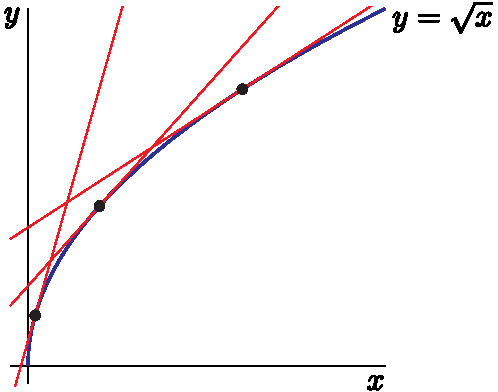
\includegraphics{tangentSqrt}
 \end{center}
\end{efig}

\end{itemize}

\end{eg}

\begin{eg}[$\diff{}{x} \left\{ |x| \right\}$]\label{eg diff abs}
Compute the derivative, $f'(a)$, of the function $f(x)=|x|$ at the point
$x=a$.
\begin{itemize}
 \item We should start this example by recalling the definition of $|x|$ (we
saw this back in Example~\ref{eg lim tricky}):
\begin{align*}
  |x| &= \begin{cases}
	 -x & \text{ if $x<0$}\\
	 0 & \text{ if $x=0$}\\
	 x & \text{ if $x>0$}.
         \end{cases}
\end{align*}
It is definitely not just ``chop off the minus sign''.
\begin{efig}
\begin{center}
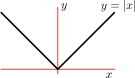
\includegraphics[height=3cm]{../limits/abs}
\end{center}
\end{efig}


\item This breaks our computation of the derivative into 3 cases depending on
whether $x$ is positive, negative or zero.
\item Assume $x>0$. Then
\begin{align*}
  \diff{f}{x}
  &= \lim_{h\to0} \frac{f(x+h)-f(x)}{h} \\
  &= \lim_{h\to0} \frac{|x+h|-|x|}{h} \\
\intertext{Since $x>0$ and we are interested in the behaviour of this function
as $h \to 0$ we can assume $h$ is much smaller than $x$. This means $x+h>0$ and
so $|x+h|=x+h$.}
  &= \lim_{h\to0} \frac{x+h-x}{h} \\
  &= \lim_{h\to0} \frac{h}{h} = 1 &\text{as expected}
\end{align*}
\item Assume $x<0$. Then
\begin{align*}
  \diff{f}{x}
  &= \lim_{h\to0} \frac{f(x+h)-f(x)}{h} \\
  &= \lim_{h\to0} \frac{|x+h|-|x|}{h} \\
\intertext{Since $x<0$ and we are interested in the behaviour of this function
as $h \to 0$ we can assume $h$ is much smaller than $x$. This means $x+h<0$ and
so $|x+h|=-(x+h)$.}
  &= \lim_{h\to0} \frac{-(x+h)-(-x)}{h} \\
  &= \lim_{h\to0} \frac{-h}{h} = -1
\end{align*}

\item When $x=0$ we have
\begin{align*}
  f'(0)
  &= \lim_{h\to0} \frac{f(0+h)-f(0)}{h} \\
  &= \lim_{h\to0} \frac{|0+h|-|0|}{h} \\
  &= \lim_{h\to0} \frac{|h|}{h}
\end{align*}
To proceed we need to know if $h>0$ or $h<0$, so we must use one-sided limits.
The limit from above is:
\begin{align*}
  \lim_{h \to 0^+} \frac{|h|}{h} &=
\lim_{h \to 0^+} \frac{h}{h} &\text{since $h>0$, $|h|=h$}\\
&= 1
\intertext{Whereas, the limit from below is:}
  \lim_{h \to 0^-} \frac{|h|}{h} &=
\lim_{h \to 0^-} \frac{-h}{h} &\text{since $h<0$, $|h|= -h$}\\
&= -1
\end{align*}
Since the one-sided limits differ, the limit as $h\to 0$ does not exist. And
thus the derivative does not exist as $x=0$.
\end{itemize}
In summary:
\begin{align*}
  \diff{}{x} |x| &= \begin{cases}
                     -1 & \text{if $x<0$} \\
                     DNE & \text{if $x=0$} \\
                     1 & \text{if $x>0$} \\
                    \end{cases}
\end{align*}
\begin{efig}
\begin{center}
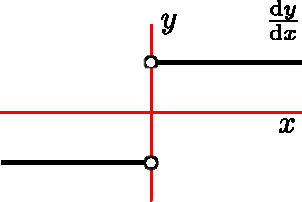
\includegraphics[height=3cm]{diff_abs}
\end{center}
\end{efig}


\end{eg}
\subsection*{Where is the Derivative Undefined?}
%%%%%%%%%%%%%%%%%%%%%%%%%%%%%%%%%%%%%%%%%%%%%%%%%%%

According to Definition \ref{def:DIFFderiv}, the derivative $f'(a)$
exists precisely when the limit
$\lim\limits_{x\rightarrow a} \frac{f(x)-f(a)}{x-a}$
exists. That limit is also the slope of the tangent
line to the curve $y=f(x)$ at $x=a$. That limit does not
exist when the curve $y=f(x)$ does not have a tangent line
at $x=a$ or when the curve does have a tangent line, but
the tangent line has infinite slope. We have already
seen some examples of this.
\begin{itemize}
\item
   In Example \ref{eg:DIFFderivXm1}, we considered the
   function $f(x)=\frac{1}{x}$. This function ``blows up'' (i.e.
   becomes infinite) at $x=0$. It does not have a tangent line at
   $x=0$ and its derivative does not exist at $x=0$.
\item
   In Example \ref{eg diff abs}, we considered the function
   $f(x)=|x|$. This function does not have a tangent line at $x=0$,
   because there is a sharp corner in the graph of $y=|x|$ at $x=0$.
   (Look at the graph in Example 2.2.10.) So the derivative
    of $f(x)=|x|$ does not exist at $x=0$.
\end{itemize}
Here are a few more examples.
\goodbreak
\begin{eg}\label{eg:DIFFderivHeavy}
Visually, the function
\begin{align*}
\begin{array}{lcr}
H(x) = \begin{cases}
           0  & \text{if }x \le 0 \\
           1 & \text{if }x>0
       \end{cases}
&\qquad&
\raisebox{-0.5\height}{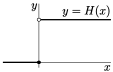
\includegraphics{heavy}}
\end{array}
\end{align*}
does not have a tangent line at $(0,0)$. Not surprisingly,
when $a=0$ and $h$ tends to $0$ with $h>0$,
\begin{align*}
\frac{H(a+h)-H(a)}{h}
=\frac{H(h)-H(0)}{h}
 =\frac{1}{h}
\end{align*}
blows up. The same sort of computation shows that
$f'(a)$ cannot possibly exist whenever the function
$f$ is not continuous at $a$. We will formalize, and prove, this statement
in Theorem \ref{thm:DIFFdiffGivesCont}, below.
\end{eg}


\begin{eg}[$\diff{}{x}x^{1/3}$]\label{eg:DIFFderivXthird}
Visually, it looks like the function $f(x) = x^{1/3}$, sketched below,
(this might be a good point to recall that cube roots of negative
numbers are negative --- for example, since $(-1)^3=-1$, the
cube root of $-1$ is $-1$),
\begin{efig}
  \begin{center}
  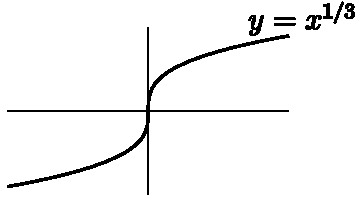
\includegraphics{Xthird}
  \end{center}
\end{efig}
has the $y$--axis as its tangent line at $(0,0)$. So we would
expect that $f'(0)$ does not exist. Let's check. With $a=0$,
\begin{align*}
f'(a)= \lim_{h\rightarrow 0}\frac{f(a+h)-f(a)}{h}
=\lim_{h\rightarrow 0}\frac{f(h)-f(0)}{h}
 =\lim_{h\rightarrow 0}\frac{h^{1/3}}{h}
 =\lim_{h\rightarrow 0}\frac{1}{h^{2/3}}
 =DNE
\end{align*}
as expected.

\end{eg}
\begin{eg}[$\diff{}{x}\sqrt{|x|}$]\label{eg:DIFFderivCusp}
We have already considered the derivative of the function
$\sqrt{x}$ in Example \ref{eg:DIFFderivXsqrt}.
We'll now look at the function $f(x) = \sqrt{|x|}$.
Recall, from Example \ref{eg diff abs}, the definition of $|x|$.
%%% Put in equation number for |x| following Figure 1.5.1
%%% Use it in place of the reference to Example 1.5.6
%%% in Example 2.2.10.
When $x>0$, we have $|x|=x$ and $f(x)$ is identical to $\sqrt{x}$.
When $x<0$, we have $|x|=-x$ and $f(x)=\sqrt{-x}$. So to graph
$y=\sqrt{|x|}$ when $x<0$, you just have to graph $y=\sqrt{x}$
for $x>0$ and then send $x\rightarrow -x$ --- i.e. reflect the
graph in the $y$--axis. Here is the graph.
\vadjust{
\begin{efig}
  \begin{center}
  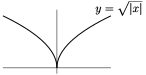
\includegraphics{XsqrtAbs}
  \end{center}
\end{efig}
}
The pointy thing at the origin is called a cusp. The graph of
$y=f(x)$ does not have a tangent line at $(0,0)$ and, correspondingly,
$f'(0)$ does not exist because
\begin{align*}
\lim_{h\rightarrow 0^+}\frac{f(h)-f(0)}{h}
 =\lim_{h\rightarrow 0^+}\frac{\sqrt{|h|}}{h}
 =\lim_{h\rightarrow 0^+}\frac{1}{\sqrt{h}}
 =DNE
\end{align*}
\end{eg}

\begin{theorem}\label{thm:DIFFdiffGivesCont}
If the function $f(x)$ is differentiable at $x=a$, then $f(x)$ is also continuous at $x=a$.
\end{theorem}
\begin{proof}
The function $f(x)$ is continuous at $x=a$ if and only if the limit of
\begin{align*}
f(a+h) - f(a) = \frac{f(a+h)-f(a)}{h}\ h
\end{align*}
as $h\rightarrow 0$ exists and is zero. But if $f(x)$ is differentiable at $x=a$, then,
as $h\rightarrow 0$,  the first factor, $ \frac{f(a+h)-f(a)}{h}$ converges to $f'(a)$
and the second factor, $h$, converges to zero. So the product provision of our
arithmetic of limits Theorem \ref{thm arith lim} implies that the product
$\frac{f(a+h)-f(a)}{h}\ h$ converges to $f'(a)\cdot 0=0$ too.
\end{proof}

Notice that while this theorem is useful as stated, it is (arguably) more often applied in its contrapositive\footnote{If you have forgotten what the contrapositive is, then quickly reread Footnote~\ref{footnote contrapositive} in Section~\ref{sec lim func}.} form:
\begin{theorem}[The contrapositive of Theorem~\ref{thm:DIFFdiffGivesCont}]
\label{thm_2_2_1}
 If $f(x)$ is not continuous at $x=a$ then it is not differentiable at $x=a$.
\end{theorem}
As the above examples illustrate, this statement does not tell us what happens if $f$ \emph{is} continuous at $x=a$ --- we have to think!

%%%%%%%%%%%%%%%%%%%%%%%%%%%%%%%%%%%%%%%%%%%%%%%%%%%
\section{Interpretations of the Derivative}\label{sec_2_3}
%%%%%%%%%%%%%%%%%%%%%%%%%%%%%%%%%%%%%%%%%%%%%%%%%%%


In the previous sections we defined the derivative as the slope of a
tangent line, using a particular limit. This allows us to compute
``the slope of a curve\footnote{Again --- recall that we are being a little sloppy
with this term --- we really mean ``The slope of the tangent line to the curve''.}'' and
provides us with one interpretation of the derivative. However, the main importance of
derivatives does not come from this application. Instead, (arguably) it comes from the
interpretation of the derivative as the instantaneous rate of change of a quantity.

%%%%%%%%%%%%%%%%%%%%%%%%%%%%%%%%%%%%%%%%%%%%%%%%%%%%%%%%%%%%%%%%%%%%%%
\subsection*{Instantaneous Rate of Change}
%%%%%%%%%%%%%%%%%%%%%%%%%%%%%%%%%%%%%%%%%%%%%%%%%%%%%%%%%%%%%%%%%%%%%%


In fact we have already (secretly) used a derivative to compute an instantaneous rate of
change in Section~\ref{sec velocity}. For your convenience we'll review that computation
here, in Example \ref{eg:DIFFfirstVelocity}, and then generalise it.

\begin{eg}\label{eg:DIFFfirstVelocity}
You drop a ball from a tall building. After $t$ seconds the ball has fallen
a distance of $s(t)=4.9 t^2$ metres. What is the velocity of the ball one
second after it is dropped?

\begin{itemize}
 \item In the time interval from $t=1$ to $t=1+h$ the ball travels
a distance
\begin{align*}
s(1+h)-s(1)=4.9 (1+h)^2 - 4.9 (1)^2
           =4.9\big[2h+h^2\big]
\end{align*}
\item So the average velocity over this time interval is
\begin{align*}
&\text{average velocity from $t=1$ to $t=1+h$} \\
&\hskip0.5in=\frac{\text{distance travelled from $t=1$ to $t=1+h$}}
       {\text{length of time from $t=1$ to $t=1+h$}} \\[5pt]
&\hskip0.5in=\frac{s(1+h)-s(1)}{h} \\
&\hskip0.5in=\frac{4.9\big[2h+h^2\big]}{h} \\
&\hskip0.5in=4.9[2+h]
\end{align*}
\item The instantaneous velocity at time $t=1$ is then defined to be the limit
\begin{align*}
&\text{instantaneous velocity at time $t=1$} \\
&\hskip0.5in=\lim_{h\rightarrow 0}
\big[\text{average velocity from $t=1$ to $t=1+h$}\big]\\
&\hskip0.5in=\lim_{h\rightarrow 0}\frac{s(1+h)-s(1)}{h} = s'(1) \\
&\hskip0.5in= \lim_{h\rightarrow 0} 4.9[2+h] \\
&\hskip0.5in= 9.8\text{m/sec}
\end{align*}
\item We conclude that the instantaneous velocity at time $t=1$,
which is the instantaneous rate of change of distance per unit time
at time $t=1$, is the derivative  $s'(1)=9.8\text{m/sec}$.
\end{itemize}

\end{eg}

Now suppose, more generally, that you are taking a walk and that
as you walk, you are continuously measuring some quantity, like temperature,
and that the measurement at time $t$ is $f(t)$. Then the
\begin{align*}
&\text{average rate of change of $f(t)$ from $t=a$ to $t=a+h$} \\
&\hskip0.5in=\frac{\text{change in $f(t)$ from $t=a$ to $t=a+h$}}
       {\text{length of time from $t=a$ to $t=a+h$}} \\[5pt]
&\hskip0.5in=\frac{f(a+h)-f(a)}{h}
\end{align*}
so the
\begin{align*}
&\text{instantaneous rate of change of $f(t)$ at $t=a$} \\
&\hskip0.5in=\lim_{h\rightarrow 0}
\big[\text{average rate of change of $f(t)$ from $t=a$ to $t=a+h$}\big]\\
&\hskip0.5in=\lim_{h\rightarrow 0}\frac{f(a+h)-f(a)}{h} \\
&\hskip0.5in= f'(a)
\end{align*}
In particular, if you are walking along the $x$--axis and your $x$--coordinate
at time $t$ is $x(t)$, then $x'(a)$ is the instantaneous rate of change
(per unit time) of your $x$--coordinate at time $t=a$, which is
your velocity at time $a$. If $v(t)$ is your velocity at time $t$, then
$v'(a)$ is the instantaneous rate of change of your velocity at time
$a$. This is called your acceleration at time $a$.

You might expect that if the instantaneous rate of change of a function at  
time $c$ is strictly positive, then, in some sense, the function is 
increasing at $t=c$. You would be right. Indeed, if $f'(c)>0$, then, by definition, the limit of $\frac{f(t)-f(c)}{t-c}$ as $t$ approaches $c$ is strictly bigger than zero. So 
\begin{itemize}
\item
for all $t>c$ that are sufficiently close\footnote{This is typical mathematician speak --- it allows us to be completely correct, without 
being terribly precise. In this context, ``sufficiently close'' means ``The following need not be true for all $t$ bigger than $c$, but there must 
exist some $b>c$ so that the following is true for all $c<t<b$''. Typically
we do not know what $b$ is. And typically it does not matter what the 
exact value of $b$ is. All that matters is that $b$ exists and is 
strictly bigger than $c$.} to $c$
  \begin{align*}
         \frac{f(t)-f(c)}{t-c}>0
          & \implies f(t)-f(c) > 0\qquad \text{(since $t-c>0$)} \\
          & \implies f(t)>f(c)
  \end{align*}
\item 
for all $t<c$ that are sufficiently close to $c$
   \begin{align*}
         \frac{f(t)-f(c)}{t-c}>0
          & \implies f(t)-f(c) < 0\qquad \text{(since $t-c<0$)} \\
          & \implies f(t)<f(c)
  \end{align*}
\end{itemize}
Consequently we say that ``$f(t)$ is increasing at $t=c$''. If we wish
to emphasise that the inequalities above are the strict inequalities
$>$ and $<$, as opposed to $\ge$ and $\le$, we will say that
``$f(t)$ is strictly increasing at $t=c$''.


%%%%%%%%%%%%%%%%%%%%%%%%%%%%%%%%%%%%%%%%%%%%%%%%%%%%%%%%%%%%%%%%%%%%%%
\subsection*{Slope}
%%%%%%%%%%%%%%%%%%%%%%%%%%%%%%%%%%%%%%%%%%%%%%%%%%%%%%%%%%%%%%%%%%%%%%

Suppose that $y=f(x)$ is the equation of a curve in the $xy$--plane.
That is, $f(x)$ is the $y$--coordinate of the point on the curve whose
$x$--coordinate is $x$. Then, as we have already seen,
\begin{align*}
\big[\text{the slope of the secant through $\big(a,f(a)\big)$
       and $\big(a+h,f(a+h)\big)$}\big]
=\frac{f(a+h)-f(a)}{h}
\end{align*}
This is shown in Figure~\ref{fig tangA} below.
\begin{fig}\label{fig tangA}
  \begin{center}
  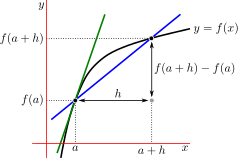
\includegraphics{extra/tangentA}
  \end{center}
\end{fig}

In order to create the tangent line (as we have done a few times now) we
squeeze $h \to 0$. As we do this, the secant through $\big(a,f(a)\big)$
and $\big(a+h,f(a+h)\big)$ approaches\footnote{We are of course
   assuming that the curve is smooth enough to have a tangent line at $a$.}
the tangent line to $y=f(x)$ at $x=a$. Since the secant becomes the
tangent line in this limit, the slope of the secant becomes the slope
of the tangent and
\begin{align*}
\big[\text{the slope of the tangent line to $y=f(x)$ at $x=a$}\big]
&=\lim_{h\rightarrow 0}\frac{f(a+h)-f(a)}{h} \\
&=f'(a).
\end{align*}


Let us go a little further and work out a general formula for the equation
of the tangent line to $y=f(x)$ at $x=a$. We know that the tangent line
\begin{itemize}
\item
   has slope $f'(a)$ and
\item
   passes through the point $\big(a, f(a)\big)$.
\end{itemize}

\noindent
There are a couple of different ways to construct the equation of the tangent
line from this information. One is to observe, as in
Figure \ref{fig:DIFFtangentEqn}, that if $(x,y)$ is any
other point on the tangent line then the line segment from $\big(a,f(a)\big)$
to $(x,y)$ is part of the tangent line and so also has slope $f'(a)$.
That is,
\begin{align*}
\frac{y- f(a)}{x-a} =\big[\text{the slope of the tangent line}\big]
  =f'(a)
\end{align*}
Cross multiplying gives us the equation of the tangent line:
\begin{align*}
y-f(a) = f'(a)\,(x-a)\qquad\text{or}\qquad
y=f(a)+f'(a)\,(x-a)
\end{align*}
\begin{fig}
\label{fig:DIFFtangentEqn}
  \begin{center}
  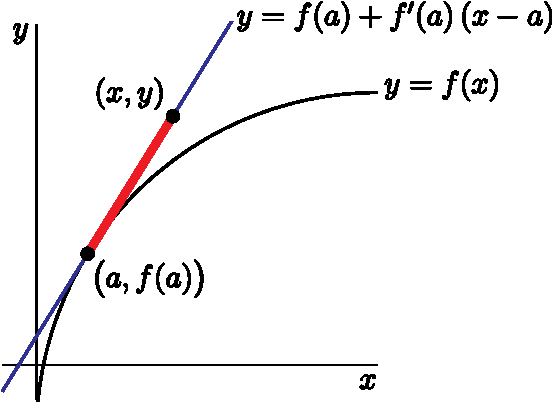
\includegraphics{tangentB}

  A line segment of a tangent line
  \end{center}
\end{fig}


A second way to derive the same equation of the same tangent line is
to recall that the general equation for a line, with finite  slope,
is $y=mx+b$, where $m$ is the slope and $b$ is the $y$-intercept.
We already know the slope --- so $m=f'(a)$. To work out $b$ we use
the other piece of information --- $(a,f(a))$ is on the line.
So $(x,y)=(a,f(a))$ must solve $y=f'(a)\,x+b$. That is,
\begin{align*}
  f(a) &= f'(a) \cdot a + b & \text{and so } &&  b&=f(a)- af'(a)
\end{align*}
Hence our equation is, once again,
\begin{align*}
  y &= f'(a) \cdot x + \left(f(a)-af'(a) \right)
            && \text{or, after rearranging a little,} \\
  y &= f(a) + f'(a) \, (x-a)
\end{align*}
This is a very useful formula, so perhaps we should make it a theorem.

\begin{theorem}[Tangent line]\label{thm:DIFFtangentLine}
 The tangent line to the curve $y=f(x)$ at $x=a$ is given by the equation
\begin{align*}
  y &= f(a) + f'(a) \, (x-a)
\end{align*}
provided the derivative $f'(a)$ exists.
\end{theorem}
The caveat at the end of the above theorem is necessary --- there are certainly cases in
which the derivative does not exist and so we do need to be careful.




\begin{eg}\label{eg:DIFFtangentA}
Find the tangent line to the curve $y=\sqrt{x}$ at $x=4$.


Rather than redoing everything from scratch, we can, and for
efficiency, should, use Theorem \ref{thm:DIFFtangentLine}.
To write this up properly, we must ensure that  we tell the reader
what we are doing. So something like the following:

\begin{itemize}
 \item By Theorem \ref{thm:DIFFtangentLine}, the tangent line to the curve
$y=f(x)$ at $x=a$ is given by
\begin{align*}
  y &= f(a) + f'(a) (x-a)
\end{align*}
provided $f'(a)$ exists.
\item In Example \ref{eg:DIFFderivXsqrt}, we found that, for any $a>0$, the derivative of
$\sqrt{x}$ at $x=a$ is
\begin{align*}
  f'(a) &= \frac{1}{2\sqrt{a}}
\end{align*}
\item In the current example, $a=4$ and we have
\begin{align*}
f(a)=f(4)=\sqrt{x}\big|_{x=4}=\sqrt{4}=2\qquad\text{and}\qquad
f'(a)=f'(4)=\frac{1}{2\sqrt{a}}\Big|_{a=4}=\frac{1}{2\sqrt{4}}=\frac{1}{4}
\end{align*}
\item So the equation of the tangent line to $y=\sqrt{x}$ at $x=4$ is
\begin{align*}
y= 2+\frac{1}{4}\,\big(x-4\big)\qquad\text{or}\qquad
y=\frac{x}{4}+1
\end{align*}
\end{itemize}
We don't have to write it up using dot-points as above; we have used them here to help
delineate each step in the process of computing the tangent line.
\end{eg}



%%%%%%%%%%%%%%%%%%%%%%%%%%%%%%%%%%%%%%%%%%%%%%%%%%%
\section{Arithmetic of Derivatives - a Differentiation Toolbox}\label{sec_2_4}
%%%%%%%%%%%%%%%%%%%%%%%%%%%%%%%%%%%%%%%%%%%%%%%%%%%

So far, we have evaluated derivatives only by applying
Definition \ref{def:DIFFderiv} to the function at hand and then computing the
required limits directly. It is quite obvious that as the function being
differentiated becomes even a little complicated, this procedure quickly becomes
extremely unwieldy. It is many orders of magnitude more efficient to have
access to
\begin{itemize}
\item a list of derivatives of some simple functions and
\item a collection of rules for breaking down complicated derivative computations
   into sequences of simple derivative computations.
\end{itemize}
This is precisely what we did to compute limits. We started with limits of
simple functions and then used ``arithmetic of limits'' to computed limits of
complicated functions.

We have already started building our list of derivatives of simple
functions. We have shown, in
Examples~\ref{eg:DIFFderivX0},~\ref{eg:DIFFderivX1},~\ref{eg:DIFFderivX2}
and~\ref{eg:DIFFderivXsqrt}, that
\begin{align*}
\diff{}{x} 1 &= 0 &
\diff{}{x} x &= 1 &
\diff{}{x} x^2 &= 2x &
\diff{}{x} \sqrt{x} &= \frac{1}{2\sqrt{x}}
\end{align*}
We'll expand this list later.

We now start building a collection of tools that help reduce the problem of computing the
derivative of a complicated function to that of computing the derivatives of a number of
simple functions. In this section we give three derivative ``rules'' as three separate
theorems. We'll give the proofs of these theorems in the next section and examples
of how they are used in the following section.

As was the case for limits, derivatives interact very cleanly with addition, subtraction
and multiplication by a constant. The following result actually follows very directly
from the first three points of Theorem~\ref{thm arith lim}.
\begin{lemma}[Derivative of sum and difference]\label{thm:DIFFaddsub}
Let $f(x),g(x)$ be differentiable functions and let $c \in \mathbb{R}$ be a constant.
Then
\begin{align*}
  \diff{}{x} \big\{ f(x)+g(x) \big\} &= f'(x)+g'(x)\\
  \diff{}{x} \big\{ f(x)-g(x)\big\} &= f'(x)-g'(x)\\
  \diff{}{x} \big\{ c f(x) \big\} &= c f'(x)
\end{align*}
That is,  the derivative of the sum is the sum of the derivatives, and so forth.
\end{lemma}
Following this we can combine the three statements in this lemma into a single rule which
captures the ``linearity of differentiation''.
\begin{theorem}[Linearity of differentiation]\label{thm:DIFFlinearity}
Again, let $f(x),g(x)$ be differentiable functions, let $\alpha, \beta \in \mathbb{R}$
be constants and define the  ``linear combination''
\begin{align*}
  S(x) &= \alpha f(x) + \beta g(x).
\end{align*}
Then the derivative of $S(x)$ at $x=a$ exists and is
\begin{align*}
  \diff{S}{x} = S'(x) &= \alpha f'(x) + \beta g'(x).
\end{align*}
Note that we can recover the three rules in the previous lemma by setting
$\alpha=\beta=1$ or $\alpha=1, \beta=-1$ or $\alpha=c$, $\beta=0$.
\end{theorem}


Unfortunately, the derivative does not act quite as simply on
products or quotients. The rules for computing derivatives of products and
quotients get their own names and theorems:

\begin{theorem}[The product rule]\label{thm:DIFFprodRule}
Let $f(x),g(x)$ be differentiable functions, then the derivative of the product
$f(x)g(x)$ exists and is given by
\begin{align*}
  \diff{}{x} \big\{ f(x) \, g(x) \big\} &= f'(x) \, g(x) + f(x) \, g'(x).
\end{align*}
\end{theorem}

Before we proceed to the derivative of the ratio of two functions, it is worth noting a
special case of the product rule when $g(x)=f(x)$. In fact, since this is a useful
special case, let us call it a corollary\footnote{Recall that a corollary is an important
result that follows from one or more theorems --- typically without too much extra work
--- as is the case here.}:
\begin{cor}[Derivative of a square]\label{cor_2_4}
Let $f(x)$ be a differentiable function, then the derivative of its square is:
\begin{align*}
  \diff{}{x} \big\{ f(x)^2 \big\} &=  2\, f(x)\, f'(x)
\end{align*}
\end{cor}
With a little work this can be generalised to other powers --- but that is best done once
we understand how to compute the derivative of the composition of two functions. That
requires the chain rule (see Theorem~\ref{thm:DIFFchainRuleV1} below). But before we get
to that, we need to see how to take the derivative of a quotient of two functions.

\begin{theorem}[The quotient rule]\label{thm:DIFFquotRule}
Let $f(x), g(x)$ be differentiable functions. Then the derivative of their quotient
is
\begin{align*}
  \diff{}{x} \left\{ \frac{f(x)}{g(x)} \right\} &=
\frac{f'(x) \, g(x) - f(x) \, g'(x)}{g(x)^2}.
\end{align*}
This derivative exists except at points where $g(x)=0$.
\end{theorem}
There is a useful special case of this theorem which we obtain by setting $f(x)=1$. In
that case, the quotient rule tells us how to compute the derivative of the reciprocal of
a function.
\begin{cor}[Derivative of a reciprocal]\label{cor diff recip}
Let $g(x)$ be a differentiable function. Then the derivative of the reciprocal of $g$ is
given by
\begin{align*}
  \diff{}{x} \left\{ \frac{1}{g(x)} \right\} &= -\frac{g'(x)}{g(x)^2}
\end{align*}
and exists except at those points where $g(x)=0$.
\end{cor}


So we have covered, sums, differences, products and quotients. This allows us
to compute derivatives of many different functions --- including polynomials
and rational functions. However we are still missing trigonometric functions
(for example), and a rule for computing derivatives of compositions. These will
follow in the near future, but there are a couple of things to do before that
--- understand where the above theorems come from, and practice using them.


%%%%%%%%%%%%%%%%%%%%%%%%%%%%%%%%%%%%%%%%%%%%%%%%%%%%%%%%%%%%%%%%%%%%%%
\section{Proofs of the Arithmetic of Derivatives}\label{sec proof arith deriv}
%%%%%%%%%%%%%%%%%%%%%%%%%%%%%%%%%%%%%%%%%%%%%%%%%%%%%%%%%%%%%%%%%%%%%%

The theorems of the previous section are not too difficult to prove from the
definition of the derivative (which we know) and the arithmetic of
limits (which we also know). In this section we show how to construct
these rules.

Throughout this section we will use our two functions $f(x)$ and $g(x)$. Since the
theorems we are going to prove all express derivatives of linear combinations, products
and quotients in terms of $f,g$ and their derivatives, it is helpful to recall the
definitions of the derivatives of $f$ and $g$:
\begin{align*}
f'(x) &=\lim_{h\to0} \frac{f(x+h)-f(x)}{h} &\text{and}&&
g'(x) &=\lim_{h\to0} \frac{g(x+h)-g(x)}{h}.
\end{align*}
Our proofs, roughly speaking, involve doing algebraic manipulations to uncover the
expressions that look like the above.


% We again fix our two functions $f(x)$ and $g(x)$. Since our proofs
% necessarily involve juggling and manipulating the formulas for the derivatives of
% $f(x)$
% and $g(x)$, we define
% \begin{align*}
% F&=\frac{f(x+h)-f(x)}{h} &\text{and}&&
% G&=\frac{g(x+h)-g(x)}{h}.
% \intertext{Using these expressions, the derivatives of $f$ and
% $g$ can be expressed as}
% \lim_{h\rightarrow 0} F &=f'(x) & \text{ and}&&
% \lim_{h\rightarrow 0} G &=g'(x).
% \end{align*}
% So this tells you that when $h$ becomes very small $F$ and $F$ should be quite close
% to the derivatives $f'(x), g'(x)$. Also note that if we take the definitions of $F, G$
% and
% multiply them by $h$, and rearrange a little, we get
% \begin{align*}
%   f(x+h) &= f(x) + h F & \text{and} &&
%   g(x+h) &= g(x) + h G
% \end{align*}

%%%%%%%%%%%%%%%%%%%%%%%%%%%%%%%%%%%%%%%%%%%%%%%%%%
\subsection*{Proof of the Linearity of Differentiation
                (Theorem \ref{thm:DIFFlinearity})}
%%%%%%%%%%%%%%%%%%%%%%%%%%%%%%%%%%%%%%%%%%%%%%%%%

Recall that in Theorem \ref{thm:DIFFlinearity} we defined
$S(x)=\alpha\,f(x)+\beta\,g(x)$, where $\alpha,\beta\in\bbbr$
are constants. We wish to compute $S'(x)$, so we start with the definition:
\begin{align*}
  S'(x) &= \lim_{h \to 0} \frac{S(x+h)-S(x)}{h}
\end{align*}
Let us concentrate on the numerator of the expression inside the limit and then come
back to the full limit in a moment. Substitute in the definition of $S(x)$:
\begin{align*}
  S(x+h)-S(x) &=
  \big[ \alpha f(x+h) + \beta g(x+h) \big] -
  \big[ \alpha f(x) + \beta g(x) \big]  &\text{collect terms} \\
&=\alpha\big[f(x+h)-f(x)]+\beta\big[g(x+h)-g(x)\big]
\end{align*}
Now it is easy to see the structures we need --- namely, we almost have the expressions
for the derivatives $f'(x)$ and $g'(x)$. Indeed, all we need to do is divide by $h$ and
take the limit. So let's finish things off.
\begin{align*}
  S'(x) &= \lim_{h \to 0} \frac{S(x+h)-S(x)}{h} & \text{from above}\\
  &= \lim_{h \to 0} \frac{\alpha\big[f(x+h)-f(x)]+\beta\big[g(x+h)-g(x)\big] }{h} \\
  &= \lim_{h \to 0} \left[ \alpha\frac{f(x+h)-f(x)}{h} + \beta\frac{g(x+h)-g(x)}{h}
\right] &\text{limit laws}\\
  &= \alpha\lim_{h \to 0} \frac{f(x+h)-f(x)}{h} + \beta\lim_{h\to0}\frac{g(x+h)-g(x)}{h}
\\
  &=\alpha f'(x) + \beta g'(x)
\end{align*}
as required.

%%%%%%%%%%%%%%%%%%%%%%%%%%%%%%%%%%%%%%%%%%%%%%%%%%%%%%%%%%%%%%%%%%%%%%
\subsection*{Proof of the Product Rule
                (Theorem \ref{thm:DIFFprodRule})}
%%%%%%%%%%%%%%%%%%%%%%%%%%%%%%%%%%%%%%%%%%%%%%%%%%%%%%%%%%%%%%%%%%%%%%
After the warm-up above, we will just jump straight in. Let $P(x)=f(x)\, g(x)$, the
product of our two functions. The derivative of the product is given by
\begin{align*}
  P'(x) &= \lim_{h \to 0} \frac{P(x+h)-P(x)}{h}
\end{align*}
Again we will focus on the numerator inside the limit and massage it into the form we
need. To simplify these manipulations, define
\begin{align*}
F(h) &= \frac{f(x+h)-f(x)}{h} & \text{ and } &&
G(h) &= \frac{g(x+h)-g(x)}{h}.
\intertext{Then we can write}
  f(x+h)&= f(x)+hF(h) &\text{and} && g(x+h)&=g(x)+hG(h).
\intertext{We can also write}
  f'(x) &= \lim_{h\to0} F(h) & \text{and}&&
  g'(x) &= \lim_{h\to0} G(h).
\end{align*}
So back to that numerator:
\begin{align*}
P(x+h)-P(x)
&=f(x+h)\cdot g(x+h)-f(x) \cdot g(x) & \text{substitute}\\
&=[f(x)+ hF(h)]\ [g(x)+hG(h)]-f(x) \cdot g(x) & \text{expand} \\
&=f(x)g(x) + f(x)\cdot hG(h) + hF(h)\cdot g(x) + h^2 F(h)\cdot G(h) -f(x) \cdot
g(x) \\
&= f(x) \cdot hG(h) + hF(h) \cdot g(x) + h^2F(h) \cdot G(h).
\end{align*}
Armed with this we return to the definition of the derivative:
\begin{align*}
P'(x)
&=\lim_{h\to 0}\frac{P(x+h)-P(x)}{h} \\
&= \lim_{h\to 0} \frac{f(x) \cdot hG(h) + hF(h) \cdot g(x) + h^2 F(h) \cdot
G(h) }{h}\\
&= \left(\lim_{h\to 0} \frac{f(x) \cdot h G(h)}{h}\right)
 + \left(\lim_{h\to 0} \frac{h F(h) \cdot g(x)}{h}\right)
 + \left(\lim_{h\to 0} \frac{h^2 F(h) \cdot G(h) }{h}\right)\\
&= \left(\lim_{h\to 0} f(x) \cdot G(h)\right)
 + \left(\lim_{h\to 0} F(h) \cdot g(x)\right)
 + \left(\lim_{h\to 0} h  F(h) \cdot G(h)\right)
\intertext{Now since $f(x)$ and $g(x)$ do not change as we send $h$ to zero, we can pull
them outside. We can also write the third term as the product of 3 limits:}
&= \left(f(x) \lim_{h\to 0} G(h)\right)
 + \left(g(x) \lim_{h\to 0} F(h)\right)
 + \left(\lim_{h\to 0} h\right)  \cdot \left(\lim_{h\to0} F(h)\right) \cdot
\left(\lim_{h\to0} G(h)\right)\\
&= f(x) \cdot g'(x) + g(x)\cdot f'(x) + 0 \cdot f'(x) \cdot g'(x) \\
&= f(x) \cdot g'(x) + g(x) \cdot f'(x).
\end{align*}
And so we recover the product rule.


%%%%%%%%%%%%%%%%%%%%%%%%%%%%%%%%%%%%%%%%%%%%%%%%%%%%%%%%%%%%%%%%%%%%%%
\subsection*{(optional) --- Proof of the Quotient Rule
                (Theorem \ref{thm:DIFFquotRule})}
%%%%%%%%%%%%%%%%%%%%%%%%%%%%%%%%%%%%%%%%%%%%%%%%%%%%%%%%%%%%%%%%%%%%%%

We now give the proof of the quotient rule in two steps\footnote{We thank
Serban Raianu for suggesting this approach.}. We assume throughout that 
$g(x) \neq 0$ and that $f(x)$ and $g(x)$ are differentiable, meaning 
that the limits defining $f'(x)$, $g'(x)$ exist.
\begin{itemize}
\item
In the first step, we prove the quotient rule under the assumption that $f(x)/g(x)$ is differentiable.
\item
In the second step, we prove that $1/g(x)$ differentiable. Once we know that 
$1/g(x)$ is differentiable, the product rule implies that $f(x)/g(x)$ is
differentiable. 
\end{itemize}

\noindent\emph{Step 1: the proof of the quotient rule assumng that 
$\frac{f(x)}{g(x)}$ is differentiable.}\ \ \ Write $Q(x)=\frac{f(x)}{g(x)}$. Then $f(x) = g(x)\,Q(x)$
so that $f'(x) = g'(x)\,Q(x) + g(x)\,Q'(x)$, by the product rule, and
\begin{align*}
Q'(x) &= \frac{f'(x)-g'(x)\,Q(x)}{g(x)}
       = \frac{f'(x)-g'(x)\,\frac{f(x)}{g(x)}}{g(x)} \\
      &= \frac{f'(x)g(x)-f(x)g'(x)}{g(x)^2}
\end{align*}

\noindent\emph{Step 2: the proof that $1/g(x)$ is differentiable.}\ \ \ 
By definition
\begin{align*}
\diff{}{x}\frac{1}{g(x)}
&=\lim_{h\rightarrow 0}\frac{1}{h}\left[\frac{1}{g(x+h)}-\frac{1}{g(x)}\right]
=\lim_{h\rightarrow 0}\frac{g(x)-g(x+h)}{h\,g(x)\,g(x+h)}
\\
&=-\lim_{h\rightarrow 0}\frac{1}{g(x)}\ \frac{1}{g(x+h)}\ 
                                        \frac{g(x+h)-g(x)}{h}\\
&=-\frac{1}{g(x)}\ 
   \lim_{h\rightarrow 0}\frac{1}{g(x+h)}\ 
   \lim_{h\rightarrow 0}\frac{g(x+h)-g(x)}{h}\\
&=-\frac{1}{g(x)^2}g'(x)
\end{align*}

%%%%%%%%%%%%%%%%%%%%%%%%%%%%%%%%%%%%%%%%%%%%%%%%%%%%%%%%%%%%%%%%%%%%%%
\section{Using the Arithmetic of Derivatives --  Examples}\label{sec_2_6}
%%%%%%%%%%%%%%%%%%%%%%%%%%%%%%%%%%%%%%%%%%%%%%%%%%%%%%%%%%%%%%%%%%%%%%
In this section we illustrate the computation of derivatives using the arithmetic of
derivatives --- Theorems~\ref{thm:DIFFlinearity},~\ref{thm:DIFFprodRule}
and~\ref{thm:DIFFquotRule}. To make it clear which rules we are using during the examples
we will note which theorem we are using:
\begin{flushleft}
\begin{tabular}{lcccr}
$\bullet$
\lin\ to stand for ``linearity'' &\quad
&$\diff{}{x}\{\alpha\,f(x)+\beta\,g(x)\} = \alpha\,f'(x)+\beta\,g'(x)$
&\quad&Theorem~\ref{thm:DIFFlinearity}
\\[2ex]
$\bullet$
\prod\ to stand for ``product rule''&\quad
&$\diff{}{x}\{f(x)\,g(x)\}=f'(x)\,g(x)+f(x)\,g'(x)$
&\quad&Theorem~\ref{thm:DIFFprodRule}
\\[2ex]
$\bullet$
\quot\ to stand for ``quotient rule''&\quad
&$\diff{}{x}\Big\{\frac{f(x)}{g(x)}\Big\}= \frac{f'(x)\,g(x)-f(x)\,g'(x)}{g(x)^2}$
&\quad&Theorem~\ref{thm:DIFFquotRule}
\end{tabular}
\end{flushleft}

We'll start with a really easy example.

\begin{eg}\label{eg:DIFFsimpleToolsAA}
  \begin{align*}
  \diff{}{x} \{ 4x + 7 \}
  &= 4 \cdot \diff{}{x} \{ x \}  + 7 \cdot \diff{}{x} \{ 1 \} & \text{LIN}\\
  &= 4 \cdot 1 + 7 \cdot 0 = 4
\end{align*}
where we have used LIN with $f(x)=x$, $g(x)=1$, $\alpha=4$, $\beta=7$.
\end{eg}

\begin{eg}\label{eg:DIFFsimpleToolsAB}
Continuing on from the previous example, we can use the product rule
and the previous result to compute
  \begin{align*}
  \diff{}{x} \big\{ x ( 4x + 7) \big\}
  &= x \cdot \diff{}{x} \{ 4x + 7 \} + (4x+7) \diff{}{x} \{ x \} &
\text{PR} \\
  &= x \cdot 4 + (4x+7) \cdot 1 \\
  &= 8x+7
\end{align*}
where we have used the product rule PR with $f(x) =x$ and $g(x)=4x+7$.
\end{eg}
\begin{eg}\label{eg:DIFFsimpleToolsAB2}
In the same vein as the previous example, we can use the quotient rule to compute
  \begin{align*}
  \diff{}{x} \left\{ \frac{x}{4x + 7} \right \}
  &= \frac{ (4x+7) \cdot \diff{}{x} \{x\}  - x \cdot \diff{}{x} \{ 4x + 7 \} }{(4x+7)^2}
& \text{QR}  \\
  &= \frac{ (4x+7) \cdot 1  - x \cdot 4 }{(4x+7)^2}  \\
&= \frac{7}{(4x+7)^2}
\end{align*}
where we have used the quotient rule QR with $f(x) =x$ and $g(x)=4x+7$.
\end{eg}


Now for a messier example.
\begin{eg}\label{eg:DIFFsimpleToolsNA}
Differentiate
\begin{align*}
f(x)&=\frac{x}{2x+\frac{1}{3x+1}}
\end{align*}

This problem looks nasty. But it isn't so hard if we just
build it up a bit at a time.
\begin{itemize}
 \item First, $f(x)$ is the ratio of
\begin{align*}
f_1(x)=x\qquad\text{and}\qquad f_2(x)=2x+\frac{1}{3x+1}
\end{align*}
If we can find the derivatives of $f_1(x)$ and $f_2(x)$, we will be able
to get the derivative of $f(x)$ just by applying the quotient rule. The derivative,
$f'_1(x)=1$, of $f_1(x)$ is easy, so let's work on  $f_2(x)$.

\item The function $f_2(x)$ is the linear combination
\begin{align*}
f_2(x)=2f_3(x)+f_4(x)\qquad\text{with}\qquad
f_3(x)=x \quad\text{and}\quad f_4(x)= \frac{1}{3x+1}
\end{align*}
If we can find the derivatives of $f_3(x)$ and $f_4(x)$, we will be able
to get the derivative of $f_2(x)$ just by applying linearity
(Theorem~\ref{thm:DIFFlinearity}). The derivative, $f'_3(x)=1$, of $f_3(x)$ is easy.
So let's work of $f_4(x)$.
\item The function $f_4(x)$ is the ratio
\begin{equation*}
f_4(x)=\frac{1}{f_5(x)}\qquad\text{with}\qquad f_5(x)=3x+1
\end{equation*}
If we can find the derivative of $f_5(x)$, we will be able to get
the derivative of $f_4(x)$ just by applying the special case
the quotient rule (Corollary~\ref{cor diff recip}). The derivative of
$f_5(x)$ is easy.

\item So we have completed breaking down $f(x)$ into easy
pieces. It is now just a matter of reversing the break down steps,
putting everything back together, starting with the easy pieces
and working up to $f(x)$. Here goes.
\begin{align*}
f_5(x)&=3x+1 &\text{ so } \diff{}{x} f_5(x) &= 3\diff{}{x} x +\diff{}{x} 1
    =3\cdot 1+0 = 3 & \text{LIN} \\[0.1in]
f_4(x)&=\frac{1}{f_5(x)}
   &\text{ so } \diff{}{x} f_4(x)&=-\frac{f'_5(x)}{f_5(x)^2}=-\frac{3}{(3x+1)^2}
                    & \text{QR} \\[0.1in]
f_2(x)&=2f_3(x)+f_4(x) &\text{ so }
    \diff{}{x} f_2(x) &= 2f'_3(x)+ f'_4(x)=2-\frac{3}{(3x+1)^2}
                    & \text{LIN} \\[0.1in]
f(x)&=\frac{f_1(x)}{f_2(x)}&\text{ so }
     \diff{}{x} f(x)&=\frac{f'_1(x)f_2(x)-f_1(x)f'_2(x)}{f_2(x)^2}
                    & \text{QR} \\
    & &             &=\frac{1\big[2x+\frac{1}{3x+1}\big]
                            -x\big[2-\frac{3}{(3x+1)^2}\big]}
                       {\big[2x+\frac{1}{3x+1}\big]^2}
\end{align*}
Oof!
\item We now have an answer. But we really should clean it up, not only to make
it easier to read, but also because invariably such computations are
just small steps inside much larger computations. Any future computations
involving this expression will be a lot easier and less error prone
if we clean it up now.
Cancelling the $2x$ and the $-2x$ in
\begin{align*}
  1\big[2x+\frac{1}{3x+1}\big]
                            -x\big[2-\frac{3}{(3x+1)^2}\big]
&=2x+\frac{1}{3x+1} -2x+\frac{3x}{(3x+1)^2} \\
&=\frac{1}{3x+1}+\frac{3x}{(3x+1)^2}
\end{align*}
and multiplying both the numerator
and denominator by $(3x+1)^2$ gives
\begin{align*}
f'(x)&=\frac{\frac{1}{3x+1}+\frac{3x}{(3x+1)^2}}
                       {\big[2x+\frac{1}{3x+1}\big]^2}
\ \frac{(3x+1)^2}{(3x+1)^2} \\[0.1in]
&=\frac{(3x+1)+3x}{\big[2x(3x+1)+1\big]^2} \\[0.1in]
&=\frac{6x+1}{[6x^2+2x+1]^2}.
\end{align*}



\end{itemize}

\end{eg}

While the linearity theorem (Theorem \ref{thm:DIFFlinearity}) is stated
for a linear combination of two functions, it is not difficult to extend it
to linear combinations of three or more functions as the following
example shows.

\begin{eg}\label{eg:DIFFsimpleToolsB}
We'll start by generalising linearity to three functions.
\begin{align*}
\diff{}{x}\big\{a F(x)+ b G(x)+ c H(x)\big\}
 &=\diff{}{x}\big\{\ a \cdot [F(x)]\ +\ 1\cdot[b G(x)+c H(x)]\ \big\} \\
   &=a F'(x)+\diff{}{x}\{b G(x)+c H(x)\} \\
   &\qquad\qquad\text{by \lin\ with $\alpha=a$, $f(x)=F(x)$, $\beta=1$,} \\
   &\qquad\qquad\text{and $g(x)=b G(x)+c H(x)$} \\
   &=a F'(x)+b G'(x)+c H'(x) \\
   &\qquad\qquad\text{by \lin\ with $\alpha=b $, $f(x)=G(x)$, $\beta=c$,} \\
   &\qquad\qquad\text{and $g(x)=H(x)$}
\end{align*}
This gives us linearity for three terms, namely (just replacing
upper case names by lower case names)
\begin{align*}
\diff{}{x}\{af(x)+bg(x)+ch(x)\} =af'(x)+bg'(x)+ch'(x)
\end{align*}
Just by repeating the above argument many
times, we may generalise to linearity for $n$ terms, for any natural number $n$:
\begin{align*}
\diff{}{x}\{a_1f_1(x)+a_2f_2(x)+\cdots+a_n f_n(x)\}
=a_1f'_1(x)+a_2f'_2(x)+\cdots+a_n f'_n(x)
\end{align*}
\end{eg}

Similarly, while the product rule is stated for the product of
two functions, it is not difficult to extend it to the product of
three or more functions as the following example shows.

\begin{eg}\label{eg:DIFFsimpleToolsA}
Once again, we'll start by generalising the product rule to three factors.
\begin{align*}
\diff{}{x}\{F(x)\,G(x)\,H(x)\}
   &=F'(x)\,G(x)\,H(x)
    +F(x)\, \diff{}{x}\{G(x)\,H(x)\} \\
   &\qquad\qquad\text{by \prod\ with $f(x)=F(x)$ and $g(x)=G(x)H(x)$} \\
   &=F'(x)\,G(x)\,H(x)
    +F(x)\, \big\{G'(x)\,H(x)+G(x)\,H'(x)\big\} \\
   &\qquad\qquad\text{by \prod\ with $f(x)=G(x)$ and $g(x)=H(x)$}
\end{align*}
This gives us a product rule for three factors, namely (just replacing
upper case names by lower case names)
\begin{align*}
\diff{}{x}\{f(x)\,g(x)\,h(x)\}
 = f'(x)\,g(x)\,h(x)
    +f(x)\,g'(x)\,h(x)+f(x)\,g(x)\,h'(x)
\end{align*}
Observe that when we differentiate a product of three factors, the answer
is a sum of three terms and in each term the derivative acts on exactly
one of the original factors. Just by repeating the above argument many
times, we may generalise the product rule to give the derivative of a product
of $n$ factors, for any natural number $n$:
\begin{align*}
\begin{split}
\diff{}{x}\{f_1(x)\,f_2(x)\,\cdots\,f_n(x)\}
 =\quad &f'_1(x)\,f_2(x)\,\cdots\,f_n(x) \\
  +&f_1(x)\,f'_2(x)\,\cdots\,f_n(x) \\
   &\qquad \qquad\vdots \\
  +&f_1(x)\,f_2(x)\,\cdots\,f'_n(x)
\end{split}
\end{align*}
We can also write the above as
\begin{align*}
\diff{}{x}\{f_1(x)\,f_2(x)\,\cdots\,f_n(x)\}
&=
\left[
\frac{f_1'(x)}{f_1(x)}+
\frac{f_2'(x)}{f_2(x)}+
\cdots
+\frac{f_n'(x)}{f_n(x)}
\right]
\cdot   f_1(x)\,f_2(x)\,\cdots\,f_n(x)
\end{align*}

When we differentiate a product of $n$ factors, the answer
is a sum of $n$ terms and in each term the derivative acts on exactly
one of the original factors. In the first term, the derivative acts on
the first of the original factors. In the second term, the derivative acts on
the second of the original factors. And so on.

If we make $f_1(x) = f_2(x) = \cdots = f_n(x) = f(x)$ then each of the
$n$ terms on the right hand side of the above equation is the
product of $f'(x)$ and exactly $n-1$ $f(x)$'s, and so is exactly
$f(x)^{n-1}\,f'(x)$. So we get the following useful result
\begin{align*}
  \diff{}{x} f(x)^n &= n\cdot  f(x)^{n-1} \cdot  f'(x).
\end{align*}
\end{eg}

This last result is quite useful, so let us write it as a lemma for future reference.
\begin{lemma}\label{lem diff ftothen}
Let $n$ be a natural number and $f$ be a differentiable function. Then
\begin{align*}
\diff{}{x} f(x)^n &= n\cdot  f(x)^{n-1} \cdot  f'(x).
\end{align*}
\end{lemma}

This immediately gives us another useful result.
\begin{eg}\label{eg:DIFFsimpleToolsC}
We can now compute the derivative of $x^n$ for any natural number $n$. Start with
Lemma~\ref{lem diff ftothen} and substitute $f(x)=x$ and $f'(x)=1$:
\begin{align*}
\diff{}{x}x^n &= n \cdot  x^{n-1} \cdot  1 = n\, x^{n-1}
\end{align*}
\end{eg}

Again --- this is a result we will come back to quite a few times in the future, so we
should make sure we can refer to it easily.  However, at present this statement only
holds  when $n$ is a positive integer. With a little more work we can extend this to
compute $x^q$ where $q$ is any positive rational number and then any rational number at
all (positive or negative). So let us hold off for a little
longer. Instead we can make it a lemma, since it will be an ingredient in quite
a few of the examples following below and in constructing the final corollary.
\begin{lemma}[Derivative of $x^n$]
\label{lem dxn}
  Let $n$ be a positive integer then
\begin{equation}\label{eq:DIFFderivXn}
\diff{}{x} x^n = n x^{n-1}
\end{equation}
\end{lemma}

Back to more examples.
\begin{eg}\label{eg:DIFFsimpleToolsD}
\begin{align*}
\diff{}{x}\big\{2x^3+4x^5\big\}
&=2\diff{}{x}\{x^3\}+4\diff{}{x}\{x^5\} \\
   &\qquad\qquad\text{by \lin\ with $\alpha=2$, $f(x)=x^3$, $\beta=4$, and $g(x)=x^5$} \\
&=2\{3x^2\}+4\{5x^4\} \\
   &\qquad\qquad\text{by  Lemma~\ref{lem dxn}, once with $n=3$, and
    once with $n=5$} \\
&=6x^2+20x^4
\end{align*}
\end{eg}


\begin{eg}\label{eg:DIFFsimpleToolsE}
In this example we'll compute $\diff{}{x}\big\{(3x+9)(x^2+4x^3)\big\}$
in two different ways. For the first, we'll start with the product rule.
\begin{align*}
\diff{}{x}\big\{(3x+9)(x^2+4x^3)\big\}
&=\Big\{\diff{}{x}(3x+9)\Big\}\ (x^2+4x^3)
   +(3x+9)\ \diff{}{x}\{x^2+4x^3\}\\
&=\big\{3\times 1+9\times 0\big\}\ (x^2+4x^3)
   +(3x+9)\ \{2x+4(3x^2)\}\\
&=3(x^2+4x^3)+(3x+9)\ (2x+12x^2)\\
&=3x^2+12x^3+(6x^2+18x+36x^3+108x^2)\\
&=18x+117x^2+48x^3
\end{align*}
For the second, we expand the product first and then differentiate.
\begin{align*}
\diff{}{x}\big\{(3x+9)(x^2+4x^3)\big\}
&=\diff{}{x}\big\{9x^2+39x^3+12x^4\big\}\\
&=9(2x)+39(3x^2)+12(4x^3)\\
&=18x+117x^2+48x^3
\end{align*}
\end{eg}

\goodbreak
\begin{eg}\label{eg:DIFFsimpleToolsH} \issue{More\\ examples\\ like this?}
\begin{align*}
\diff{}{x}\bigg\{\frac{4x^3-7x}{4x^2+1}\bigg\}
&=\frac{(12x^2-7)(4x^2+1)-(4x^3-7x)(8x)}{(4x^2+1)^2} \\
   &\qquad\qquad\text{by \quot\ with $f(x)=4x^3-7x$, $f'(x)=12x^2-7$,} \\
   &\qquad\qquad\text{and  $g(x)=4x^2+1$, $g'(x)=8x$} \\
&=\frac{(48x^4-16x^2-7)-(32x^4-56x^2)}{(4x^2+1)^2} \\
&=\frac{16x^4+40 x^2-7}{(4x^2+1)^2}
\end{align*}
\end{eg}


\begin{eg}\label{eg:DIFFsimpleToolsF}
In this example, we'll use a little trickery to find the derivative
of $\root{3}\of{x}$. The trickery consists of observing that,
by the definition of the cube root,
\begin{align*}
x= \left(\root{3}\of{x}\right)^3.
\end{align*}
Since both sides of the expression are the same, they must have the same derivatives:
\begin{align*}
\diff{}{x}\left\{x\right\}
= \diff{}{x}\left(\root{3}\of{x}\right)^3.
\end{align*}
We already know by Theorem~\ref{thm:DIFFbasicderivs} that
\begin{align*}
\diff{}{x}\big\{x\big\}=1
\end{align*}
and that, by Lemma~\ref{lem diff ftothen} with $n=3$ and $f(x)=\root{3}\of{x}$,
\begin{align*}
\diff{}{x}\big(\root{3}\of{x}\big)^3
 = 3\ \big(\root{3}\of{x}\big)^2\cdot \diff{}{x}\big\{\root{3}\of{x}\big\}
 = 3\,x^{2/3}\cdot \diff{}{x}\big\{\root{3}\of{x}\big\}.
\end{align*}
Since we know that $\diff{}{x}\left\{x\right\}
= \diff{}{x}\left(\root{3}\of{x}\right)^3$, we must have
\begin{align*}
1=3x^{2/3}\cdot \diff{}{x}\big\{\root{3}\of{x}\big\}
\intertext{which we can rearrange to give the result we need}
\diff{}{x}\big\{\root{3}\of{x}\big\} &=\tfrac{1}{3} x^{-2/3}
\end{align*}
\end{eg}


\begin{eg}\label{eg:DIFFsimpleToolsG}
In this example, we'll use the same trickery as in Example
\ref{eg:DIFFsimpleToolsF} to find the derivative $x^{p/q}$
for any two natural numbers $p$ and $q$. By definition
of the $q^{\rm th}$ root,
\begin{align*}
x^p= \big(x^{p/q}\big)^q.
\end{align*}
That is, $x^p$ and  $\big(x^{p/q}\big)^q$ are the same function, and so have the same
derivative. So we differentiate both of them. We already know that, by Lemma \ref{lem
dxn}
with $n=p$,
\begin{align*}
\diff{}{x}\big\{x^p\big\}=p x^{p-1}
\end{align*}
and that, by Lemma~\ref{lem diff ftothen} with $n=q$ and $f(x)=x^{p/q}$,
\begin{align*}
\diff{}{x}\big\{\big(x^{p/q}\big)^q\big\}
& = q\ \big(x^{p/q}\big)^{q-1}\ \diff{}{x}\big\{x^{p/q}\big\}
\end{align*}
Remember that $(x^a)^b = x^{(a \cdot b)}$. Now these two derivatives
must be the same. So
\begin{align*}
p x^{p-1} &=q\cdot x^{(pq-p)/q} \diff{}{x}\big\{x^{p/q}\big\} \\
\intertext{and, rearranging things,}
\diff{}{x}\big\{x^{p/q}\big\}
   & =\frac{p}{q} x^{p-1-(pq-p)/q} \\[0.05in]
   & =\frac{p}{q} x^{(pq-q-pq+p)/q} \\[0.05in]
   & =\frac{p}{q} x^{\nicefrac{p}{q}-1}
\end{align*}
So finally
\begin{align}\label{eq:DIFFxpoverq}
  \diff{}{x} \left\{ x^{p/q} \right\} &= \frac{p}{q} x^{\nicefrac{p}{q} -1 }
\end{align}
Notice that this has the same form as Lemma \ref{lem dxn}, above,
except with $n=\nicefrac{p}{q}$ allowed to be any positive rational
number, not just a positive integer.
\end{eg}



\begin{eg}[Derivative of $x^{-m}$]\label{eg:DIFFsimpleToolsI}
In this example we'll use the quotient rule to find the derivative of
$x^{-m}$, for any natural number $m$.

By the special case of the quotient rule (Corollary~\ref{cor diff recip}) with $g(x)=x^m$
and $g'(x)=mx^{m-1}$
\begin{align*}
\diff{}{x}\big\{x^{-m}\big\}
=\diff{}{x}\bigg\{\frac{1}{x^m}\bigg\}
=-\,\frac{mx^{m-1}}{{(x^m)}^2}
=-m x^{-m-1}
\end{align*}
Again, notice that this has the same form as Lemma~\ref{lem dxn},
above, except with $n=-m$ being a negative integer.
\end{eg}

\begin{eg}\label{eg:DIFFsimpleToolsJ}
In this example we'll use the quotient rule to find the derivative of
$x^{-p/q}$, for any pair of natural numbers $p$ and $q$. By the special case
the quotient rule (Corollary~\ref{cor diff recip}) with
$g(x)=x^{\nicefrac{p}{q}}$ and $g'(x)=\frac{p}{q}x^{\nicefrac{p}{q}-1}$,
\begin{align*}
\diff{}{x}\big\{x^{-\nicefrac{p}{q}}\big\}
=\diff{}{x}\bigg\{\frac{1}{x^{\nicefrac{p}{q}}}\bigg\}
=-\,\frac{\frac{p}{q}x^{\nicefrac{p}{q}-1}}{{(x^{\nicefrac{p}{q}})}^2}
=-\frac{p}{q}\ x^{-\nicefrac{p}{q}-1}
\end{align*}
\end{eg}

Note that we have found, in Examples \ref{eg:DIFFderivX0},
\ref{eg:DIFFsimpleToolsG} and \ref{eg:DIFFsimpleToolsJ},
the derivative of $x^a$ for any rational number $a$, whether
0, positive, negative, integer or fractional. In all cases, the answer
is
\begin{cor}[Derivative of $x^a$]\label{cor:DIFFxtoa}
  Let $a$ be a rational number, then
\begin{equation}
\diff{}{x} x^a = a x^{a-1}
\end{equation}
\end{cor}
\noindent We shall show, in Example \ref{eg diff power}, that the formula 
$\diff{}{x} x^a = a x^{a-1}$ in fact applies for all real numbers $a$, not just rational numbers.

Back in Example~\ref{eg:DIFFderivXsqrt} we computed the derivative of $\sqrt{x}$ from the
definition of the derivative. The above corollary (correctly) gives
\begin{align*}
  \diff{}{x} x^{\nicefrac{1}{2}} &= \frac{1}{2} x^{-\nicefrac{1}{2}}
\end{align*}
but with far less work.


Here's an (optional) messy example.
\begin{eg}[Optional messy example]\label{eg:DIFFsimpleToolsNB}
Find the derivative of
\begin{equation*}
f(x)=\frac{(\sqrt{x}-1)(2-x)(1-x^2)}{\sqrt{x}(3+2x)}
\end{equation*}

\begin{itemize}
 \item As we seen before, the best strategy for dealing with nasty
expressions is to break them up into easy pieces. We can think of
$f(x)$ as the five--fold product
\begin{equation*}
f(x)=f_1(x)\cdot f_2(x)\cdot f_3(x)\cdot \frac{1}{f_4(x)}\cdot \frac{1}{f_5(x)}
\end{equation*}
with
\begin{align*}
f_1(x)=\sqrt{x}-1\quad
f_2(x)=2-x\quad
f_3(x)=1-x^2\quad
f_4(x)=\sqrt{x}\quad
f_5(x)=3+2x
\end{align*}
\item By now, the derivatives of the $f_j$'s should be easy to find:
\begin{align*}
f'_1(x)=\frac{1}{2\sqrt{x}}\quad
f'_2(x)=-1\quad
f'_3(x)=-2x\quad
f'_4(x)=\frac{1}{2\sqrt{x}}\quad
f'_5(x)=2
\end{align*}
\item Now, to get the derivative $f(x)$ we use the $n$--fold product rule which was
developed in Example~\ref{eg:DIFFsimpleToolsA}, together with the special case
of the quotient rule (Corollary~\ref{cor diff recip}).
\begin{align*}
f'(x)&=f'_1f_2f_3\frac{1}{f_4}\frac{1}{f_5}
+f_1f'_2f_3\frac{1}{f_4}\frac{1}{f_5}
+f_1f_2f'_3\frac{1}{f_4}\frac{1}{f_5}
-f_1f_2f_3\frac{f'_4}{f^2_4}\frac{1}{f_5}
-f_1f_2f_3\frac{1}{f_4}\frac{f'_5}{f^2_5}\\[0.1in]
&=\Big[\frac{f'_1}{f_1}+\frac{f'_2}{f_2}+\frac{f'_3}{f_3}-\frac{f'_4}{f_4}
-\frac{f'_5}{f_5}\Big]f_1f_2f_3\frac{1}{f_4}\frac{1}{f_5}\\[5mm]
&=\bigg[\frac{1}{2\sqrt{x}(\sqrt{x}-1)}
       -\frac{1}{2-x}-\frac{2x}{1-x^2}-\frac{1}{2x}
-\frac{2}{3+2x}\bigg]\frac{(\sqrt{x}-1)(2-x)(1-x^2)}{\sqrt{x}(3+2x)}
\end{align*}
The trick that we used in going from the first line to the second line,
namely multiplying term number $j$ by $\frac{f_j(x)}{f_j(x)}$
is often useful in simplifying the derivative of a product of many
factors\footnote{Also take a look at ``logarithmic differentiation'' in
Section~\ref{sec diff logs}.}.
\end{itemize}

\end{eg}


%%%%%%%%%%%%%%%%%%%%%%%%%%%%%%%%%%%%%%%%%%%%%%%%%%%%%%%%%%%%%%%%%%%%%%
\section{Derivatives of Exponential Functions}\label{sec exp func}
%%%%%%%%%%%%%%%%%%%%%%%%%%%%%%%%%%%%%%%%%%%%%%%%%%%%%%%%%%%%%%%%%%%%%%
Now that we understand how derivatives interact with products and quotients, we
are able to compute derivatives of
\begin{itemize}
 \item polynomials,
 \item rational functions, and
 \item powers and roots of rational functions.
\end{itemize}
Notice that all of the above come from knowing\footnote{Differentiating powers
and roots of functions is actually quite a bit easier once one knows the chain
rule --- which we will discuss soon.} the derivative of $x^n$ and applying
linearity of derivatives and the product rule.

There is still one more ``rule'' that we need to complete our toolbox and that
is the chain rule. However before we get there, we will add a few functions
to our list of things we can differentiate\footnote{One reason we add these
functions is that they interact very nicely with the derivative. Another
reason is that they turn up in many ``real world'' examples.}. The
first of these is the exponential function.


Let $a>0$ and set $f(x) = a^x$ --- this is what is known as an
exponential function. Let's see what happens when we try to compute
the derivative of this function just using the definition of the derivative.
\begin{align*}
  \diff{f}{x} &= \lim_{h \to 0} \frac{f(x+h) - f(x)}{h}
  = \lim_{h \to 0} \frac{a^{x+h} - a^x}{h} \\
  &= \lim_{h \to 0} a^x \cdot \frac{a^{h} - 1}{h}
  = a^x \cdot \lim_{h \to 0} \frac{a^{h} - 1}{h}
\end{align*}
Unfortunately we cannot complete this computation because we cannot evaluate the
last
limit directly. For the moment, let us assume this limit exists and name it
\begin{align*}
  C(a) &= \lim_{h \to 0} \frac{a^{h} - 1}{h}
\end{align*}
It depends only on $a$ and is completely independent of $x$. Using  this
notation (which
we will quickly improve upon below), our desired derivative is now
\begin{align*}
  \diff{}{x}a^x &=  C(a)\cdot a^x.
\end{align*}
Thus the derivative of $a^x$ is $a^x$ multiplied by some constant --- i.e. the
function
$a^x$ is nearly unchanged by differentiating. If we can tune $a$ so that $C(a) =
1$ then the derivative would just be the original function! This turns out to be
very useful.

To try finding an $a$ that obeys $C(a)=1$, let us investigate how $C(a)$ changes
with
$a$. Unfortunately (though this fact is not at all obvious) there is no way to
write
$C(a)$ as a finite combination of any of the functions we have examined
so far\footnote{To a bit more be precise, we say that a number $q$ is algebraic
if we can
write $q$ as the zero of a polynomial with integer coefficients. When $a$ is any
positive
algebraic number other $1$, $C(a)$ is not algebraic. A number that is not
algebraic is
called transcendental. The best known example of a transcendental number is
$\pi$ (which
follows from the Lindemann-Weierstrass Theorem --- way beyond the scope of this
course).}. To get started, we'll try to guess $C(a)$, for a few values of
$a$, by plugging in some small values of $h$.
\begin{eg}\label{eg log est}
Let $a =1$ then $C(1) = \ds \lim_{h \to 0} \frac{1^h-1}{h} = 0$. This is not
surprising
since $1^x=1$ is constant, and so its derivative must be zero everywhere. Let $a
=2$
then $C(2) = \ds \lim_{h \to 0} \frac{2^h-1}{h}$. Setting $h$ to smaller and
smaller
numbers gives
%\begin{center}
% \begin{tabular}{|c||c|c|c|c|c|c|c|}
%\hline
%  $h$ & 1 & 0.1 & 0.01 & 0.001 & 0.0001 & $\cdots$ & keep going \\
%\hline
%  $\frac{2^h-1}{h}$ & 1 & 0.71773463 & 0.69555501 & 0.69338746 & 0.69317120 &
%$\cdots$ & 0.69314718\\
%\hline
% \end{tabular}
%\end{center}
\begin{center}
   \renewcommand{\arraystretch}{1.2}
   \begin{tabular}{|c||c|c|c|c|c|c|c|}
       \hline
       $h$ & 0.1 & 0.01 & 0.001 & 0.0001 & 0.00001 & 0.000001 & 0.0000001 \\
       \hline
       $\tfrac{2^h-1}{h}$ & 0.7177 & 0.6956 & 0.6934 & 0.6932 &
             0.6931 & 0.6931 & 0.6931 \\ \hline
     \end{tabular}
     \renewcommand{\arraystretch}{1.0}
\end{center}
Similarly when $a=3$ we get
%\begin{center}
% \begin{tabular}{|c||c|c|c|c|c|c|c|}
%\hline
%  $h$ & 1 & 0.1 & 0.01 & 0.001 & 0.0001 & $\cdots$ & keep going \\
%\hline
%  $\frac{3^h-1}{h}$ & 2 & 1.1612317 & 1.1046692 & 1.0992160 & 1.0986726 &
%$\cdots$ & 1.0986123 \\
%\hline
% \end{tabular}
%\end{center}
\begin{center}
   \renewcommand{\arraystretch}{1.2}
   \begin{tabular}{|c||c|c|c|c|c|c|c|}
       \hline
       $h$ & 0.1 & 0.01 & 0.001 & 0.0001 & 0.00001 & 0.000001 & 0.0000001 \\
       \hline
       $\tfrac{3^h-1}{h}$ & 1.1612 & 1.1047 & 1.0992 & 1.0987 &
             1.0986 & 1.0986 & 1.0986 \\ \hline
     \end{tabular}
     \renewcommand{\arraystretch}{1.0}
\end{center}
and $a=10$
\begin{center}
   \renewcommand{\arraystretch}{1.2}
   \begin{tabular}{|c||c|c|c|c|c|c|c|}
       \hline
       $h$ & 0.1 & 0.01 & 0.001 & 0.0001 & 0.00001 & 0.000001 & 0.0000001 \\
       \hline
       $\tfrac{10^h-1}{h}$ & 2.5893 & 2.3293 & 2.3052 & 2.3028 &
             2.3026 & 2.3026 & 2.3026 \\ \hline
     \end{tabular}
     \renewcommand{\arraystretch}{1.0}
\end{center}
% \intremark{ %%%%%%%%%%%%%%%%%%%%%%%%%%%%%%
% Under IEEE 754 double precision has  a precision of 53 bits, which
% corresponds to about 15.9 decimal digits. See
% {\tt http://en.wikipedia.org/wiki/Floating\_point}. If, for example
% $10^{0.000001}$ is accurate to 14 significant digits
% \begin{equation*}
% \frac{1.00000abcdefgh-1}{0.000001}
% =\frac{0.00000abcdefgh}{0.000001}
% =a.bcdefgh
% \end{equation*}
% is accurate to 7 decimal places.
%
% \renewcommand{\arraystretch}{1.2}
% \begin{center}
%      \begin{tabular}{|c|c|}
%           \hline
%              $h$ & $\tfrac{10^h-1}{h}$\\ \hline
%              0.1 & 2.5892541 \\ \hline
%              0.01 & 2.3292992 \\ \hline
%              0.001 & 2.3052381 \\ \hline
%              0.0001 & 2.3028502 \\ \hline
%              0.00001 & 2.3026116 \\ \hline
%              0.000001 & 2.3025877 \\ \hline
%              0.0000001 & 2.302585 \\ \hline
%      \end{tabular}
% \end{center}
% \renewcommand{\arraystretch}{1.0}
%
% \begin{center}
%  \begin{tabular}{|c||c|c|c|c|c|c|c|}
% \hline
%   $h$ & 1 & 0.1 & 0.01 & 0.001 & 0.0001 & $\cdots$ & keep going \\
% \hline
%   $\frac{10^h-1}{h}$ & 9 & 2.5892541 & 2.3292992 & 2.3052381 & 2.3028502 &
% $\cdots$ & 2.3025851 \\
% \hline
%  \end{tabular}
% \end{center}
% }%%%%%%%%%%%%%%%%%%%%%%%%%%%%
From this example it appears that $C(a)$ increases as we increase $a$,
and that $C(a) = 1$ for some value of $a$ between $2$ and $3$.
\end{eg}


We can learn a lot more about $C(a)$, and, in particular, confirm the
guesses that we made in the last example, by making use of logarithms ---
this would be a good time for you to review them.

% \subsection*{Whirlwind Review of Logarithms}
% Before you read much further into this little review on logarithms, you should
% first go
% back and take a look at the review of inverse functions in Section~\ref{sec
% inverse
% functions}.
% \subsubsection*{Logarithmic Functions}
% For any $0 < q < 1$, the function $q^x$ is strictly decreasing\footnote{If
% $x_0<x_1$ then
% $q^{x_0}>q^{x_1}$.}. While for any $q>1$ the function is strictly
% increasing\footnote{If
% $x_0<x_1$ then $q^{x_0}>q^{x_1}$.}. This means for any $q>0, q\neq 1$, we have
% (by the
% horizontal line test), $f(x) = q^x$ is a one-to-one function. Hence it has an
% inverse
% function.
% \begin{defn}
%  Let $q>0$ with $q \neq 1$. Then the logarithm with base $q$ is defined by
%  \begin{align*}
%   y=\log_q(x) & \liff x=q^y
% \end{align*}
% \end{defn}
% Since $\log_q(x)$ and $q^x$ are inverses of each other, we have
% \begin{align*}
%   \log_q( q^x ) &=x & q^{\log_q(x)} &=x
% \end{align*}
% Remember your logarithms
% \begin{align*}
%   \log_q(xy) &= \log_q(x) + \log_q(y) \\
%   \log_q(x/y) &= \log_q(x) - \log_q(y) \\
%   \log_q( x^r ) &= r \log_q (x)
% \end{align*}
%
% Can we convert from logarithms in one base to logarithms in another. For
% example, if
% our calculator does logarithms base 10 (which it very likely does), how can we
% compute a logarithm base $q$?
% \begin{align*}
%   \log_q(x) &= \frac{\log_{10} x}{\log_{10} q}
% \end{align*}
% How did we get this? Well, let's start with a number $x$ and we want to compute
% $y =
% \log_q x$. Hence
% \begin{align*}
%     y &= \log_q x
% \intertext{We can rearrange this by exponentiating both sides}
%   q^y &= q^{\log_q x} = x
% \intertext{Now take log base 10 of both sides}
%   \log_{10} q^y &= \log_{10} x \\
% \intertext{But recall that $\log ( x^r ) = r \log (x)$, so}
%   y \log_{10} q &= \log_{10} x \\
%   y &= \frac{\log_{10} x}{\log_{10} q}
% \end{align*}

\subsection*{Whirlwind Review of Logarithms}
Before you read much further into this little review on logarithms,
you should first go back and take a look at the review of inverse
functions in Section~\ref{sec inverse  functions}.
\subsubsection*{Logarithmic Functions}
We are about to define the ``logarithm with base $q$''.
In principle, $q$ is allowed to be any strictly positive real
number, except $q=1$. However we shall restrict our attention
to $q>1$, because, in practice, the only $q$'s that are ever
used are $e$ (a number that we shall define in the next few pages),
$10$ and, if you are a computer scientist, $2$.
So, fix any $q>1$ (if you like, pretend that $q=10$). The function
$f(x)=q^x$
\begin{itemize}
\item increases as $x$ increases (for example if $x'>x$, then
                          $10^{x'} = 10^x \cdot 10^{x'-x} >10^x$ since
                          $10^{x'-x}>1$)
\item obeys $\lim\limits_{x\rightarrow-\infty} q^x=0$ (for
                        example $10^{-1000}$ is really small) and
\item obeys $\lim\limits_{x\rightarrow+\infty} q^x=+\infty$ (for
                        example $10^{+1000}$ is really big).
\end{itemize}
Consequently, for any $0<Y<\infty$, the horizontal straight line
$y=Y$ crosses the graph of $y=f(x)=q^x$ at exactly one point,
as illustrated in the figure below.
\vadjust{
\begin{efig}
  \begin{center}
  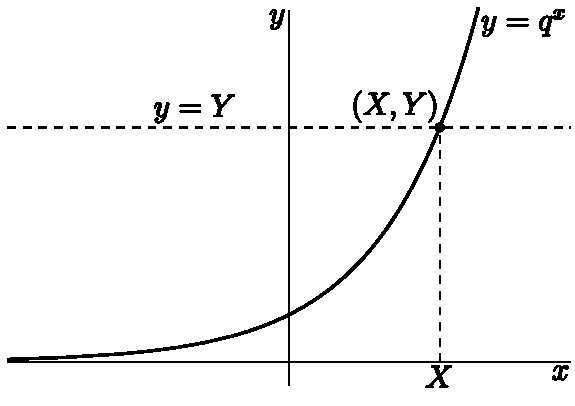
\includegraphics{expGraphB}
  \end{center}
\end{efig}
}
The $x$--coordinate of that
intersection point, denoted $X$ in the figure, is $\log_q(Y)$.
So $\log_q(Y)$ is the power to which you have to raise $q$ to get $Y$.
It is the inverse function of $f(x)=q^x$. Of course we are free
to rename the dummy variables $X$ and $Y$. If, for example,
we wish to graph our logarithm function, it is natural to rename
$Y\rightarrow x$ and $X\rightarrow y$, giving
\begin{defn}\label{def_2_7_1}
Let $q>1$. Then the logarithm with base $q$ is defined\footnote{
We can also define logarithms with base $0<r<1$ but doing so is not necessary.
To see this, set $q=1/r>1$. Then it is reasonable to define $\log_r(x) = -
\log_q(x)$ since
\begin{align*}
  r^{\log_r(x)}
  &= \left(\frac{1}{q}\right)^{\log_r(x)}
  = \left(\frac{1}{q}\right)^{-\log_q(x)}
  = q^{\log_q(x)} = x
\end{align*}
as required.
} by
 \begin{align*}
  y=\log_q(x) & \liff x=q^y
\end{align*}
\end{defn}
Obviously the power to which we have to raise $q$ to get $q^x$
           is $x$, so we have both
\begin{align*}
  \log_q( q^x ) &=x & q^{\log_q(x)} &=x
\end{align*}
From the exponential properties
 \begin{alignat*}{4}
   q^{log_q(xy)} &= xy &&= q^{log_q(x)} q^{log_q(y)} = q^{log_q(x)+log_q(y)} \\
  q^{log_q(x/y)} &= x/y&&= q^{log_q(x)} / q^{log_q(y)} = q^{log_q(x)-log_q(y)}
    \\
  q^{log_q(x^r)} &= x^r &&= \big(q^{log_q(x)}\big)^r = q^{r log_q(x)}
\end{alignat*}
 we have
\begin{align*}
  \log_q(xy) &= \log_q(x) + \log_q(y) \\
  \log_q(x/y) &= \log_q(x) - \log_q(y) \\
  \log_q( x^r ) &= r \log_q (x)
\end{align*}

Can we convert from logarithms in one base to logarithms in another?
For example, if our calculator computes logarithms base 10 for
us (which it very likely does), can we also use it to compute a
logarithm base $q$? Yes, using
\begin{align*}
  \log_q(x) &= \frac{\log_{10} x}{\log_{10} q}
\end{align*}
How did we get this? Well, let's start with a number $x$ and suppose
that we want to compute
\begin{align*}
    y &= \log_q x
\intertext{We can rearrange this by exponentiating both sides}
  q^y &= q^{\log_q x} = x
\intertext{Now take log base 10 of both sides}
  \log_{10} q^y &= \log_{10} x \\
\intertext{But recall that $\log_q( x^r ) = r \log_q(x)$, so}
  y \log_{10} q &= \log_{10} x \\
  y &= \frac{\log_{10} x}{\log_{10} q}
\end{align*}


\subsection*{Back to that Limit}
Recall that we are trying to choose $a$ so that
\begin{align*}
  \lim_{h\to0} \frac{a^h-1}{h} &= C(a) = 1.
\end{align*}
We can estimate the correct value of $a$ by using our numerical estimate of
$C(10)$
above. The way to do this is to first rewrite $C(a)$ in terms of logarithms.
\begin{align*}
  a&= 10^{\log_{10} a} & \text{ and so }&& a^h &= 10^{h\log_{10} a}.
\end{align*}
Using this we rewrite $C(a)$ as
\begin{align*}
  C(a) &= \lim_{h\to0} \frac{1}{h} \left( 10^{h\log_{10} a}-1 \right)
\intertext{Now set $H = h\log_{10}(a)$, and notice that as $h\to 0$ we also have
$H \to
0$}
&= \lim_{H \to 0} \frac{\log_{10} a}{H} \left(10^H-1\right) \\
&= \log_{10} a \cdot \lim_{H \to 0} \frac{10^H-1}{H}\\
&= \log_{10} a \cdot C(10).
\end{align*}
Below is a sketch of $C(a)$ against $a$.
\begin{fig}\label{fig CofA2}
\begin{center}
    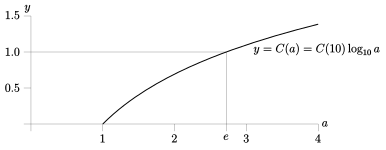
\includegraphics{CofA2}
\end{center}
\end{fig}
Remember that we are trying to find an $a$ with $C(a)=1$. We can do so by
recognising that
$C(a)=C(10)\,(\log_{10}a)$ has the following properties.
\begin{itemize}
\item When $a=1$, $\log_{10}(a) = \log_{10} 1 =0$ so that $C(a) = C(10)
\log_{10}(a) = 0$. Of course, we should have expected this,
because when $a=1$ we have $a^x = 1^x = 1$ which is just the constant
function and $\diff{}{x} 1 = 0$.

\item $\log_{10}a$ increases as $a$ increases, and hence $C(a)=C(10)\
\log_{10}a$ increases as $a$ increases.

\item $\log_{10}a$ tends to $+\infty$ as $a\rightarrow\infty$,
and hence $C(a)$  tends to $+\infty$ as $a\rightarrow\infty$.
\end{itemize}
Hence the graph of $C(a)$ passes through $(1,0)$, is always increasing as $a$
increases and goes off to $+\infty$  as $a$ goes off to $+\infty$. See Figure~\ref{fig
CofA2}. Consequently\footnote{We are applying the Intermediate Value Theorem here,
but we have neglected to verify the hypothesis that $\log_{10}(a)$
is a continuous function. Please forgive us --- we could do this if we really
had to, but it would make a big mess without adding much understanding, if we were to do
so here in the text. Better to just trust us on this.} there is exactly one value of $a$
for which
$C(a) = 1$.

The value of $a$ for which $C(a)=1$ is given the name $e$. It is called Euler's
constant\footnote{Unfortunately there is another Euler's constant, $\gamma$,
which is more properly called the  Euler--Mascheroni constant. Anyway like many
mathematical discoveries, $e$ was first found by someone else --- Napier used the
constant $e$ in order to compute logarithms but only implicitly. Bernoulli was probably
the first to approximate it when examining continuous compound interest. It first
appeared explicitly in work of Leibniz, though he denoted it $b$. It was Euler, though,
who established the notation we now use and who showed how important the constant is to
mathematics.}. % Above,
In Example~\ref{eg log est}, we estimated $C(10)\approx 2.3026$. So if we
assume
$C(a)=1$ then the above equation becomes
\begin{align*}
  2.3026 \cdot \log_{10} a &\approx 1 \\
  \log_{10} a &\approx \frac{1}{2.3026} \approx 0.4343 \\
  a &\approx 10^{0.4343} \approx 2.7813
\end{align*}
This gives us the estimate $a \approx 2.7813$ which is not too bad. In
fact\footnote{Recall $n$ factorial, written $n!$ is the product
$n\times(n-1)\times(n-2)\times\cdots\times2\times1$.}
\begin{impeqn}[Euler's constant]\label{eq:eulerconst}
\begin{align*}
e &= 2.7182818284590452354\dots\\
  &= 1 + \frac{1}{1!} + \frac{1}{2!} + \frac{1}{3!} + \frac{1}{4!} + \cdots
\end{align*}
\end{impeqn}
We will be able to explain this last formula once we develop Taylor polynomials
later in
the course.

To summarise
\begin{theorem}\label{thm_2_7_1}
The constant $e$ is the unique real number that satisfies
\begin{align*}
	\lim_{h \to 0} \frac{e^h-1}{h} &= 1
\end{align*}
Further,
\begin{align*}
	\bdiff{e^x}{x} &= e^x
\end{align*}
\end{theorem}
We plot $e^x$ in the graph below
\begin{fig}
\begin{center}
    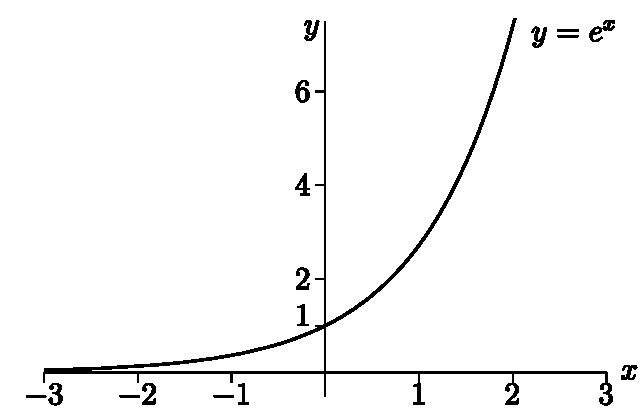
\includegraphics{expGraph}
\end{center}
\end{fig}
And just a reminder of some of its\footnote{"The function $e^x$ is of course the special
case of the function $a^x$ with $a = e$. So it inherits all the usual algebraic properties
of $a^x$."} properties\dots
\begin{enumerate}
\item $e^0=1$
\item $e^{x+y}=e^xe^y$
\item $e^{-x}=\tfrac{1}{e^x}$
\item $\big(e^x\big)^y=e^{xy}$
\item $\lim\limits_{x\rightarrow\infty}e^x=\infty$,
           $\lim\limits_{x\rightarrow-\infty}e^x=0$
\end{enumerate}

Now consider again the problem of differentiating $a^x$. We saw above that
\begin{align*}
  \diff{}{x} a^x &= C(a) \cdot a^x & \text{ and }
  C(a) &= C(10) \cdot \log_{10} a & \text{ which gives}
  \diff{}{x} a^x &= C(10)\cdot \log_{10} a \cdot a^x
\end{align*}
We can eliminate the $C(10)$ term with a little care. Since we know that $\diff{}{x} e^x
= e^x$, we have $C(e)=1$. This allows us to express
\begin{align*}
  1 = C(e) &= C(10) \cdot \log_{10} e & \text{ and so} \\
  C(10) &= \frac{1}{\log_{10} e}
\end{align*}
Putting things back together gives
\begin{align*}
  \diff{}{x} a^x &= \frac{\log_{10} a}{\log_{10} e} \cdot a^x \\
  &= \log_e a \cdot a^x.
\end{align*}
There is more than one way to get to this result. For example, let $f(x) =
a^x$, then
\begin{align*}
  \log_e f(x) &= x \log_e a \\
  f(x) &= e^{ x \log_e a}
\end{align*}
So if we write $g(x) = e^x$ then we are really attempting to differentiate the
function
\begin{align*}
  \diff{f}{x} &= \diff{}{x} g(x \cdot \log_e a).
\end{align*}
In order to compute this derivative we need to know how to differentiate
\begin{align*}
  \diff{}{x} g( q x)
\end{align*}
where $q$ is a constant. We'll hold off on learning this for the moment until
we have introduced the chain rule (see Section~\ref{sec chain rule} and in
particular Corollary~\ref{cor f of axb}). Similarly we'd like to know how to
differentiate logarithms --- again this has to wait until we have learned the
chain rule.


Notice that the derivatives
\begin{align*}
  \diff{}{x} x^n &= n x^{n-1} & \text{ and }&&
  \diff{}{x} e^x &= e^x
\end{align*}
are either nearly unchanged or actually unchanged by differentiating. It turns
out that some of the trigonometric functions also have this property of being
``nearly unchanged'' by differentiation. That brings us to the next section.


%%%%%%%%%%%%%%%%%%%%%%%%%%%%%%%%%%%%%%%%%%%%%%%%%%%%%%%%%%%%%%%%%%%%%%
\section{Derivatives of Trigonometric Functions} \label{sec diff trig}
%%%%%%%%%%%%%%%%%%%%%%%%%%%%%%%%%%%%%%%%%%%%%%%%%%%%%%%%%%%%%%%%%%%%%%
We are now going to compute the derivatives of the various trigonometric
functions, $\sin x$, $\cos x$ and so on. The computations are more involved
than the others that we have done so far and will take several steps.
Fortunately, the final answers will be very simple.

Observe that we only need to work out the derivatives
of $\sin x$ and $\cos x$, since the other trigonometric functions are really just
quotients of these two functions. Recall:
\begin{align*}
  \tan x &= \frac{\sin x}{\cos x} &
  \cot x &= \frac{\cos x}{\sin x} &
  \csc x &= \frac{1}{\sin x} &
  \sec x &= \frac{1}{\cos x}.
\end{align*}

The first steps towards computing the derivatives of $\sin x, \cos x$ is
to find their derivatives at $x=0$. The derivatives at general points $x$
will follow quickly from these, using trig identities. It is important to note
that we must measure angles in radians\footnote{In science, radians is
the standard unit for measuring angles. While you may be more familiar
with degrees, radians should be used in any computation involving calculus.
Using degrees will cause errors.
Thankfully it is easy to translate between these two measures since $360^\circ
= 2\pi$ radians. See Appendix~\ref{ssec rad deg}.}, rather than
degrees, in what follows. Indeed --- unless
explicitly stated otherwise, any number that is put into a trigonometric
function is measured in radians.


\subsection*{These Proofs are Optional, the Results are Not.}
While we expect you to read and follow these proofs, we do not expect you to be able to
reproduce them. You will be required to know the results, in particular
Theorem~\ref{thm:DIFFtrigDerivs} below.

%%%%%%%%%%%%%%%%%%%%%%%%%%%%%%%%%%%%%%%%%%%%%%%%%%%%%%%%%%%%%%%%%%%%%%
\subsection*{Step 1: $\mathbf{\diff{}{x} \{ \sin x \} \big|_{x=0}}$}
%%%%%%%%%%%%%%%%%%%%%%%%%%%%%%%%%%%%%%%%%%%%%%%%%%%%%%%%%%%%%%%%%%%%%%

By definition, the derivative of $\sin x$ evaluated at $x=0$ is
\begin{align*}
\diff{}{x} \{ \sin x \} \Big|_{x=0}
=\lim_{h\rightarrow 0}\frac{\sin h-\sin 0}{h}
=\lim_{h\rightarrow 0}\frac{\sin h}{h}
\end{align*}
We will prove this limit by use of the squeeze theorem (Theorem~\ref{thm squeeze}). To
get there we will first need to do some geometry. But first we will build some intuition.

The figure below contains part of a circle of radius 1. Recall that
an arc of length $h$ on such a circle subtends an angle of $h$
\textbf{radians} at the centre of the circle.
So the darkened arc in the figure has length $h$ and the darkened vertical
line in the figure has length $\sin h$. We must determine what happens
to the ratio of the lengths of the darkened vertical line
and darkened arc as $h$ tends to zero.

\begin{efig}
\begin{center}
     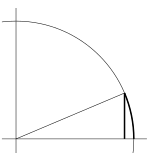
\includegraphics{sinDerivL}\qquad
     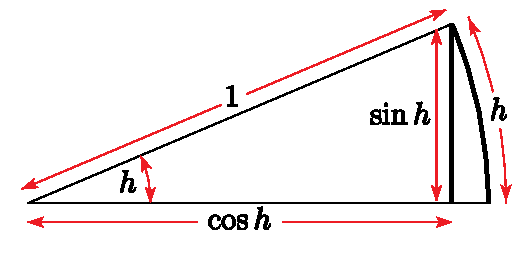
\includegraphics{sinDerivR}
\end{center}
\end{efig}

\noindent Here is a magnified version of the part of the above figure
that contains the darkened arc and vertical line.

\begin{efig}
\begin{center}
     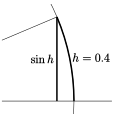
\includegraphics{sinDeriv2}
\end{center}
\end{efig}


\noindent This particular figure has been drawn with $h=.4$ radians.
Here are three more such blow ups. In  each successive figure, the
value of $h$ is smaller.
To make the figures clearer, the degree of magnification was increased
each time $h$ was decreased.

\begin{wfig}
\begin{center}
     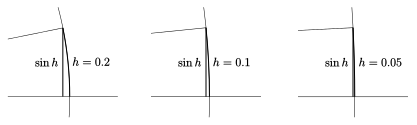
\includegraphics{sinDeriv345}
\end{center}
\end{wfig}

\noindent
As we make $h$ smaller and smaller and look at the figure with ever increasing
magnification, the arc of length $h$ and vertical line of length $\sin h$
look more and more alike. We would guess from this that
\begin{equation*}
\lim_{h\rightarrow 0}\frac{\sin h}{h}=1
\end{equation*}
The following tables of values
\renewcommand{\arraystretch}{1.1}
\begin{center}
     \begin{tabular}{|c|c|c|}
          \hline
          $h$ &     $\sin h$ &     $\tfrac{\sin h}{h}$ \\ \hline
          0.4 &      .3894 &          .9735 \\
          0.2 &      .1987 &          .9934  \\
          0.1 &      .09983 &         .9983  \\
          0.05 &     .049979 &        .99958  \\
          0.01 &     .00999983 &      .999983  \\
          0.001 &    .0099999983 &    .9999983  \\ \hline
     \end{tabular}
     \qquad\qquad
     \begin{tabular}{|c|c|c|}
          \hline
           h  &     $\sin h$ &     $\tfrac{\sin h}{h}$ \\ \hline
          $-0.4$ &      $-.3894$ &          .9735 \\
          $-0.2$ &      $-.1987$ &          .9934  \\
          $-0.1$ &      $-.09983$ &         .9983  \\
          $-0.05$ &     $-.049979$ &        .99958  \\
          $-0.01$ &     $-.00999983$ &      .999983  \\
          $-0.001$ &    $-.0099999983$ &    .9999983  \\ \hline
     \end{tabular}

\end{center}
\renewcommand{\arraystretch}{1.0}
suggests the same guess. Here is an argument that shows that the guess
really is correct.

\subsubsection{Proof that $\mathbf{\lim\limits_{h\rightarrow 0}\tfrac{\sin h}{h}=1}$:}

\begin{efig}
\begin{center}
     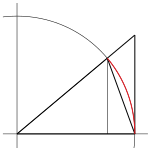
\includegraphics{sinDeriv6L}\ \ \
     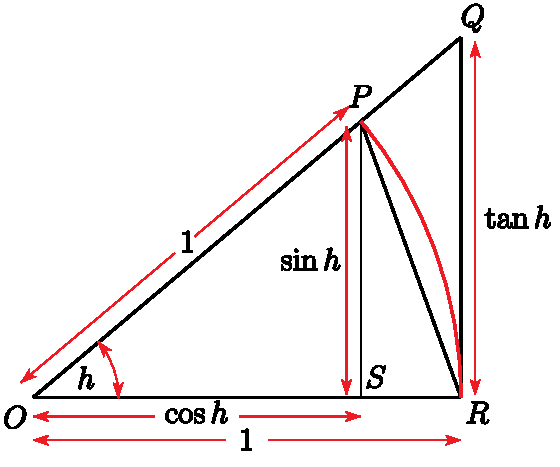
\includegraphics{sinDeriv6RR}
\end{center}
\end{efig}


\noindent The circle in the figure above has radius $1$. Hence
\begin{align*}
|OP|=|OR|&=1 &
|PS|&=\sin h\\
|OS|&= \cos h &
|QR|&=\tan h
\end{align*}
Now we can use a few geometric facts about this figure to establish both
an upper bound and a lower bound on $\frac{\sin h}{h}$ with both the upper
and lower bounds tending to $1$ as $h$ tends to $0$. So the squeeze
theorem will tell us that $\frac{\sin h}{h}$ also tends to $1$ as $h$
tends to $0$.
\begin{itemize}
 \item The triangle $OPR$ has base $1$ and height $\sin h$, and hence
\begin{align*}
\text{area of }\triangle OPR &= \half\times1\times\sin h=\frac{\sin h}{2}.
\end{align*}
 \item The triangle $OQR$ has base $1$ and height $\tan h$, and hence
\begin{align*}
\text{area of }\triangle OQR &= \half\times1\times\tan h=\frac{\tan h}{2}.
\end{align*}
 \item The ``piece of pie'' $OPR$ cut out of the circle  is the fraction
$\frac{h}{2\pi}$ of the whole circle (since the angle at the corner of
the piece of pie is $h$ radians and the angle for the whole circle is
$2\pi$ radians). Since the circle has radius $1$ we have
\begin{align*}
\text{area of pie } OPR &=
\frac{h}{2\pi} \cdot
(\text{area of circle}) = \frac{h}{2\pi} \pi \cdot 1^2= \frac{h}{2}
\end{align*}
\end{itemize}
Now the triangle $OPR$ is contained inside the piece of pie $OPR$. and so the area of the
triangle is smaller than the area of the piece of pie. Similarly, the piece of pie $OPR$
is contained inside the triangle $OQR$. Thus we have
\begin{align*}
  \text{area of triangle } OPR \leq \text{ area of pie } OPR
                              \leq \text{ area of triangle } OQR
\end{align*}
Substituting in the areas we worked out gives
\begin{align*}
  \frac{\sin h}{2}  &\leq \frac{h}{2}  \leq \frac{\tan h}{2}  \\
\intertext{which cleans up to give}
  \sin h  &\leq h  \leq \frac{\sin h}{\cos h} % \label{eqn trig sqz}
\end{align*}
We rewrite these two inequalities so that $\frac{\sin h}{h}$ appears in
both.
\begin{itemize}
 \item Since $\sin h \leq h$, we have that $\ds \frac{\sin h}{h} \leq 1$.
\item Since $\ds h \leq \frac{\sin h}{\cos h}$ we have that $\ds \cos h \leq
\frac{\sin h}{h}$.
\end{itemize}
Thus we arrive at the ``squeezable'' inequality
\begin{align*}
  \cos h \leq \frac{\sin h}{h} \leq 1
\end{align*}
We know\footnote{Again, refresh your memory by looking up Appendix~\ref{app sec
trig graphs}.} that
\begin{align*}
  \lim_{h \to 0} \cos h &=1.
\end{align*}
Since $\tfrac{\sin h}{h}$ is sandwiched between $\cos h$ and 1, we can apply the
squeeze theorem for limits (Theorem~\ref{thm squeeze}) to deduce the following lemma:
\begin{lemma}
\label{lem sinhoverh}
\begin{align*}
  \lim_{h \to 0} \frac{\sin h}{h} &= 1.
\end{align*}
\end{lemma}


Since this argument took a bit of work, perhaps we should remind ourselves why
we needed it in the first place. We were computing
\begin{align*}
  \diff{}{x} \{ \sin x\}\Big|_{x=0}
  &= \lim_{h \to 0} \frac{\sin h - \sin 0}{h}  \\
  &= \lim_{h \to 0} \frac{\sin h}{h} & \text{(This is why!)}\\
  &= 1
\end{align*}


\noindent This concludes Step 1. We now know that
$\diff{}{x}\sin x\big|_{x=0}=1$. The remaining steps are easier.

\goodbreak
%%%%%%%%%%%%%%%%%%%%%%%%%%%%%%%%%%%%%%%%%%%%%%%%%%%%%%%%%%%%%%%%%%%%%%
\subsection*{Step 2: $\mathbf{\diff{}{x} \{ \cos x \} \big|_{x=0}}$}
%%%%%%%%%%%%%%%%%%%%%%%%%%%%%%%%%%%%%%%%%%%%%%%%%%%%%%%%%%%%%%%%%%%%%%

By definition, the derivative of $\cos x$ evaluated at $x=0$ is
\begin{align*}
\lim_{h\rightarrow 0}\frac{\cos h-\cos 0}{h}
&=\lim_{h\rightarrow 0}\frac{\cos h - 1}{h}
\end{align*}
Fortunately we don't have to wade through geometry like we did for the previous step.
Instead we can recycle our work and massage the above limit to rewrite it in terms of
expressions involving $\frac{\sin h}{h}$. Thanks to Lemma~\ref{lem sinhoverh} the work
is then easy.


We'll show you two ways to proceed --- one uses a method similar to ``multiplying by the
conjugate'' that we have already used a few times (see Example~\ref{eg zero cancel limit
harder} and~\ref{eg:DIFFderivXsqrt} ), while the other uses a nice trick involving
the double--angle formula\footnote{See Appendix~\ref{sec must deriv} if you have
forgotten. You should also recall that $\sin^2\theta + \cos^2\theta =
1$. Sorry for nagging.}.

\subsubsection{Method 1 --- Multiply by the ``Conjugate''}
Start by multiplying the expression inside the limit by 1, written as
$\ds \frac{\cos h + 1}{\cos h +1}$:
\begin{align*}
  \frac{\cos h - 1}{h}
  &= \frac{\cos h - 1}{h} \cdot\frac{\cos h + 1}{\cos h +1}\\
  &= \frac{\cos^2 h - 1}{h (1+ \cos h)}
           &&\text{$\big($since $(a-b)(a+b)=a^2-b^2\big)$}\\
  &= -\frac{\sin^2 h}{h(1+\cos h)}
           &&\text{(since $\sin^2 h + \cos^2 h=1$)} \\
  &= - \frac{\sin h}{h} \cdot \frac{\sin h}{1 + \cos h}
\end{align*}
Now we can take the limit as $h \to 0$ via Lemma~\ref{lem sinhoverh}.
\begin{align*}
 \lim_{h \to 0} \frac{\cos h - 1}{h}
  &= \lim_{h \to 0} \left( \frac{-\sin h}{h} \cdot \frac{\sin h}{1 + \cos h}
\right)\\
  &= -\lim_{h \to 0}\left( \frac{\sin h}{h} \right) \cdot \lim_{h \to0}
\left( \frac{\sin h}{1 + \cos h} \right) \\
  &= - 1 \cdot \frac{0}{2} \\
  &= 0
\end{align*}

\subsubsection{ Method 2 --- via the Double Angle Formula}
The other way involves the double angle formula\footnote{We hope you looked this up
in in Appendix~\ref{sec must deriv}. Nag.},
\begin{align*}
  \cos 2\theta = 1 - 2 \sin^2(\theta) \qquad\text{or}\qquad
  \cos 2\theta -1 = - 2 \sin^2(\theta)
\end{align*}
Setting $\theta = h/2$, we have
\begin{align*}
\frac{\cos h - 1}{h}
  &= \frac{-2\big(\sin\tfrac{h}{2}\big)^2}{h}
\intertext{Now this begins to look like $\frac{\sin h}{h}$, except that inside
the $\sin(\cdot)$ we have $h/2$. So, setting $\theta =h/2$,}
\frac{\cos h - 1}{h}   &= - \frac{\sin^2 \theta}{\theta}
  = - \theta \cdot\frac{ \sin^2 \theta}{\theta^2} \\
  &= - \theta \cdot \frac{\sin \theta}{\theta} \cdot \frac{\sin \theta}{\theta}
\end{align*}
When we take the limit as $h \to 0$, we are also taking the limit as
$\theta=h/2 \to 0$, and so
\begin{align*}
\lim_{h \to 0} \frac{\cos h - 1}{h}
  &= \lim_{\theta \to 0} \left[
  - \theta \cdot \frac{\sin \theta}{\theta} \cdot \frac{\sin \theta}{\theta}
\right]\\
  &= \lim_{\theta \to 0} \left[- \theta \right]
  \cdot \lim_{\theta \to 0} \left[\frac{\sin \theta}{\theta}\right]
  \cdot \lim_{\theta \to 0} \left[\frac{\sin \theta}{\theta}\right] \\
  &= 0 \cdot 1 \cdot 1 \\
  &= 0
\end{align*}
where we have used the fact that $\ds \lim_{h \to 0} \frac{\sin h}{h} = 1$ and
that the limit of a product is the product of limits (i.e. Lemma~\ref{lem sinhoverh} and
Theorem~\ref{thm arith lim}).

Thus we have now produced two proofs of the following lemma:
\begin{lemma}\label{lem_2_8_1}
\begin{align*}
  \lim_{h \to 0} \frac{\cos h -1}{h} &= 0
\end{align*}
\end{lemma}
Again, there has been a bit of work to get to here, so we should remind ourselves why we
needed it. We were computing
\begin{align*}
  \diff{}{x} \{ \cos x \} \Big|_{x=0}
&= \lim_{h \to 0} \frac{\cos h - \cos 0}{h} \\
&= \lim_{h \to 0} \frac{\cos h - 1}{h} \\
&= 0
\end{align*}

Armed with these results we can now build up the derivatives of sine and
cosine.
\goodbreak
%%%%%%%%%%%%%%%%%%%%%%%%%%%%%%%%%%%%%%%%%%%%%%%%%%%%%%%%%%%%%%%%%%%%%%
\subsection*{Step 3: $\diff{}{x} \{ \sin x \}$ and $\diff{}{x} \{ \cos x\}$
for General $x$}
%%%%%%%%%%%%%%%%%%%%%%%%%%%%%%%%%%%%%%%%%%%%%%%%%%%%%%%%%%%%%%%%%%%%%%
To proceed to the general derivatives of $\sin x$ and $\cos x$
we are going to use the above
two results and a couple of trig identities. Remember the addition
formulae\footnote{You really should. Look this up in Appendix~\ref{sec trig add} if you
have forgotten.}
\begin{align*}
  \sin(a+b) &= \sin(a) \cos(b) + \cos(a) \sin(b)\\
  \cos(a+b) &= \cos(a) \cos(b) - \sin(a) \sin(b)
\end{align*}
To compute the derivative of $\sin(x)$ we just start from the definition of the
derivative:
\begin{align*}
\diff{}{x}\sin x
&=\lim_{h\rightarrow 0}\frac{\sin (x+h)-\sin x}{h} \\[0.05in]
&=\lim_{h\rightarrow 0}\frac{\sin x\cos h +\cos x\sin h-\sin x}{h} \\[0.05in]
&=\lim_{h\rightarrow 0}\bigg[\sin x\frac{\cos h-1}{h}
                            +\cos x\frac{\sin h-0}{h}\bigg] \\[0.05in]
&=\sin x\ \lim_{h\rightarrow 0}\frac{\cos h-1}{h}
  \ +\ \cos x\ \lim_{h\rightarrow 0}\frac{\sin h-0}{h} \\[0.05in]
&=\sin x\ \underbrace{\bigg[\diff{}{x}\cos x\bigg]_{x=0}}_{=0}
  \ +\ \cos x\ \underbrace{\bigg[\diff{}{x}\sin x\bigg]_{x=0}}_{=1} \\
&=\cos x
\end{align*}
The computation of the derivative of $\cos x$ is very similar.
\begin{align*}
\diff{}{x}\cos x
&=\lim_{h\rightarrow 0}\frac{\cos (x+h)-\cos x}{h} \\[0.05in]
&=\lim_{h\rightarrow 0}\frac{\cos x\cos h -\sin x\sin h-\cos x}{h} \\[0.05in]
&=\lim_{h\rightarrow 0}\bigg[\cos x\frac{\cos h-1}{h}
                            -\sin x\frac{\sin h-0}{h}\bigg] \\[0.05in]
&=\cos x\ \lim_{h\rightarrow 0}\frac{\cos h-1}{h}
  \ -\ \sin x\ \lim_{h\rightarrow 0}\frac{\sin h-0}{h} \\[0.05in]
&=\cos x\ \underbrace{\bigg[\diff{}{x}\cos x\bigg]_{x=0}}_{=0}
  \ -\ \sin x\ \underbrace{\bigg[\diff{}{x}\sin x\bigg]_{x=0}}_{=1} \\
&=-\sin x
\end{align*}
We have now found the derivatives of both $\sin x$ and $\cos x$,
\textit{provided $x$ is measured in radians}.

\begin{lemma}\label{lem DIFFsincos}
\begin{align*}
\diff{}{x}\sin x &=\cos x &
\diff{}{x}\cos x &=-\sin x
\end{align*}
The above formulas hold provided $x$ is measured in radians.
\end{lemma}
These formulae are pretty easy to remember --- applying $\diff{}{x}$
to $\sin x$ and $\cos x$ just exchanges $\sin x$ and $\cos x$, except for
the minus sign\footnote{There is a bad pun somewhere in here about sine errors and sign
errors.} in the derivative of $\cos x$.

\begin{remark}[Optional --- Another derivation of $\diff{}{x}\cos x =-\sin x$]
\label{rem deriv cos prime}

We remark that, once one knows that $\diff{}{x}\sin x =\cos x$, it is easy to use it and the trig identity $\cos(x) = \sin\big(\frac{\pi}{2}-x\big)$ to derive $\diff{}{x}\cos x =-\sin x$. Here is how\footnote{We thank Serban Raianu for suggesting that we include this.}. 
\begin{align*}
\diff{}{x}\cos x
&=\lim_{h\rightarrow 0}\frac{\cos (x+h)-\cos x}{h} 
=\lim_{h\rightarrow 0}\frac{\sin\big(\frac{\pi}{2}-x-h)
        -\sin\big(\frac{\pi}{2}- x\big)}{h} 
\\
&=-\lim_{h'\rightarrow 0}\frac{\sin\big(x'+h')-\sin(x')}{h'} 
\qquad\text{with }x'=\tfrac{\pi}{2}-x,\ h'=-h
\\
&=-\diff{}{x'}\sin x'\Big|_{x'=\tfrac{\pi}{2}-x}
=-\cos\big(\tfrac{\pi}{2}- x\big)
\\
&=-\sin x
\end{align*}  


\end{remark}

Note that, if $x$ is measured in degrees, then the formulas of 
Lemma \ref{lem DIFFsincos} are wrong. There
are similar formulas, but we need the chain rule to build them --- that is the
subject of the next section. But first we should find the
derivatives of the other trig functions.

\goodbreak
%%%%%%%%%%%%%%%%%%%%%%%%%%%%%%%%%%%%%%%%%%%%%%%%%%%%%%%%%%%%%%%%%%%%%%
\subsection*{Step 4: the Remaining Trigonometric Functions}
%%%%%%%%%%%%%%%%%%%%%%%%%%%%%%%%%%%%%%%%%%%%%%%%%%%%%%%%%%%%%%%%%%%%%%

It is now an easy matter to get the derivatives of the remaining
trigonometric functions using basic trig identities and the
quotient rule. Remember\footnote{You really should. If you do not then take a
quick look at the appropriate appendix.} that
\begin{align*}
  \tan x&=  \frac{\sin x}{\cos x} & \cot x &= \frac{\cos x}{\sin x}=
\frac{1}{\tan x} \\
  \csc x&=  \frac{1}{\sin x} & \sec x &= \frac{1}{\cos x}
\end{align*}
So, by the quotient rule,
\begin{alignat*}{7}
\diff{}{x}\tan x
&=\diff{}{x}\,\frac{\sin x}{\cos x} &
&=\frac{ \overbrace{\big({\ts\diff{}{x}}\sin x\big)}^{\cos x}\cos x
       -\sin x\overbrace{\big({\ts\diff{}{x}\cos x}\big)}^{-\sin x}}
                         {\cos^2 x} &
&=\sec^2 x \\[0.05in]
%%%%%%%%%%%%
\diff{}{x}\,\csc x
&=\diff{}{x}\,\frac{1}{\sin x} &
&=-\frac{ \overbrace{\big({\ts\diff{}{x}}\sin x\big)}^{\cos x}}
                         {\sin^2 x} &
&=-\csc x\cot x \\[0.05in]
%%%%%%%%%%%%
\diff{}{x}\,\sec x
&=\diff{}{x}\,\frac{1}{\cos x} &
&=-\frac{\overbrace{\big({\ts\diff{}{x}}\cos x\big)}^{-\sin x}}
                         {\cos^2 x} &
&=\sec x\tan x \\[0.05in]
%%%%%%%%%%%%
\diff{}{x}\cot x
&=\diff{}{x}\,\frac{\cos x}{\sin x} &
&=\frac{ \overbrace{\big({\ts\diff{}{x}}\cos x\big)}^{-\sin x}\sin x
       -\cos x\overbrace{{\ts\big(\diff{}{x}}\sin x\big)}^{\cos x}}
                         {\sin^2 x} &
&=-\csc^2 x
\end{alignat*}

\goodbreak
%%%%%%%%%%%%%%%%%%%%%%%%%%%%%%%%%%%%%%%%%%%%%%%%%%%%%%%%%%%%%%%%%%%%%%
\subsection*{Summary}
%%%%%%%%%%%%%%%%%%%%%%%%%%%%%%%%%%%%%%%%%%%%%%%%%%%%%%%%%%%%%%%%%%%%%%
To summarise all this work, we can write this up as a theorem:
\begin{theorem}[Derivatives of trigonometric functions]\label{thm:DIFFtrigDerivs}
 The derivatives of $\sin x$ and $\cos x$ are
\begin{align*}
  \diff{}{x} \sin x &= \cos x & \diff{}{x} \cos x &= - \sin x
\end{align*}
Consequently the derivatives of the other trigonometric functions are
\begin{align*}
  \diff{}{x} \tan x &= \sec^2 x &
  \diff{}{x} \cot x &= -\csc^2 x \\
  \diff{}{x} \csc x &= -\csc x \cot x &
  \diff{}{x} \sec x &= \sec x \tan x
\end{align*}
\end{theorem}
Of these 6 derivatives you should really memorise those of sine, cosine and tangent. We
certainly expect you to be able to work out those of cotangent, cosecant and secant.


%%%%%%%%%%%%%%%%%%%%%%%%%%%%%%%%%%%%%%%%%%%%%%%%%%%%%%%%%%%%%%%%%%%%%%
\section{One More Tool  -- the Chain Rule}\label{sec chain rule}
%%%%%%%%%%%%%%%%%%%%%%%%%%%%%%%%%%%%%%%%%%%%%%%%%%%%%%%%%%%%%%%%%%%%%%

We have built up most of the tools that we need to express derivatives of
complicated functions in terms of derivatives of simpler known functions.
We started by learning how to evaluate
\begin{itemize}
 \item derivatives of sums, products and quotients
 \item derivatives of constants and monomials
\end{itemize}
These tools allow us to compute derivatives of polynomials and
rational functions. In the previous sections, we added exponential and trigonometric
functions to our list. The final tool we add is called the chain rule.
It tells us how to take the derivative of a composition of two functions.
That is if we know $f(x)$ and $g(x)$ and their derivatives, then the chain
rule tells us the derivative of $f\big(g(x)\big)$.

Before we get to the statement of the rule, let us look at an
example showing how such a composition might arise (in the  ``real-world'').

\begin{eg}
\label{eg:DIFFcampfire}
You are out in the woods after a long day of mathematics and are
walking towards your camp fire on a beautiful still night. The heat
from the fire means that the air temperature depends on your position.
Let your position at time $t$ be $x(t)$. The temperature of the air
at position $x$ is $f(x)$. What instantaneous rate of change of
temperature do you feel at time~$t$?
\begin{efig}
\begin{center}
 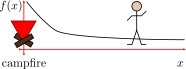
\includegraphics[width=0.8\textwidth]{campfire2}
\end{center}
\end{efig}
\begin{itemize}
 \item Because your position at time $t$ is $x=x(t)$, the temperature you feel
at time $t$ is $F(t)=f\big(x(t)\big)$.
\item The instantaneous rate of change of temperature that you feel is $F'(t)$. We have a
complicated function, $F(t)$, constructed by composing two simpler functions, $x(t)$ and
$f(x)$.
\item We wish to compute the derivative, $F'(t) = \diff{}{t} f( x(t) )$,
of the complicated function $F(t)$ in terms of the derivatives,  $x'(t)$
and $f'(x)$, of the two simple functions. This is exactly what the
chain rule does.
\end{itemize}
\end{eg}


%%%%%%%%%%%%%%%%%%%%%%%%%%%%%%%%%%%%%%%%%%%%%%%%%%%%%%%%%%%%%%%%%%%%%%
\subsection*{Statement of the Chain Rule}
%%%%%%%%%%%%%%%%%%%%%%%%%%%%%%%%%%%%%%%%%%%%%%%%%%%%%%%%%%%%%%%%%%%%%%

\begin{theorem}[The chain rule  --- version 1]
\label{thm:DIFFchainRuleV1}
  Let $a \in \mathbb{R}$ and let $g(x)$ be a function that is differentiable at
$x=a$. Now let $f(u)$ be a function that is differentiable at
$u=g(a)$. Then the function $F(x) = f(g(x))$ is differentiable at $x=a$ and
\begin{align*}
  F'(a) &=f'\big(g(a)\big)\,g'(a)
\end{align*}
\end{theorem}
Here, as was the case earlier in this chapter,  we have been very
careful to give the point at which the derivative is evaluated a special
name (i.e. $a$). But of course this evaluation point can really be
any point (where the derivative is defined).
So it is very common to just call the evaluation point ``$x$'' rather
than give it a special name like ``$a$'', like this:
\begin{theorem}[The chain rule --- version 2]
\label{thm:DIFFchainRuleV2}
 Let $f$ and $g$ be differentiable functions then
  \begin{align*}
  \diff{}{x} f\big( g( x) \big) &= f'\big(g(x)\big) \cdot g'(x)
\end{align*}
\end{theorem}
Notice that when we form the composition $f\big(g(x)\big)$ there
is an ``outside'' function (namely $f(x)$) and an ``inside'' function
(namely $g(x)$). The chain rule tells us that when we differentiate
a composition that we have to differentiate the outside and then
multiply by the derivative of the inside.
\begin{align*}
  \diff{}{x} f\big( g( x) \big)
   &= \underbrace{f'\big(g(x)\big)}_\text{diff outside} \cdot
                          \underbrace{g'(x)}_\text{diff inside}
\end{align*}
Here is another statement of the chain rule which makes this idea more
explicit.


\begin{theorem}[The chain rule --- version 3]
\label{thm:DIFFchainRuleV3}
  Let $y = f(u)$ and $u = g(x)$ be differentiable functions, then
  \begin{align*}
  \diff{y}{x} &= \diff{y}{u} \cdot \diff{u}{x}
\end{align*}
\end{theorem}
This particular form is easy to remember because it looks like we can just
``cancel'' the $\mathrm{d}u$ between the two terms.
  \begin{align*}
  \diff{y}{x} &= \frac{\mathrm{d}{y}}{\cancel{\mathrm{d}u}} \cdot
\frac{\cancel{\mathrm{d}{u}}}{\mathrm{d}x}
\end{align*}

Of course,  $\mathrm{d}u$ is not, by itself, a number or variable\footnote{In
this context $\mathrm{d}u$ is called a differential. There are ways to
understand and manipulate these in calculus but they are beyond the scope of
this course.} that can be cancelled. But this is still a good memory aid.

The hardest part about applying the chain rule is recognising
when the function you are trying to differentiate is really
the composition of two simpler functions. This takes a little practice.
We can warm up with a couple of simple examples.

\begin{eg}\label{eg:DIFFchainruleA}
 Let $f(u) = u^5$ and $g(x) = \sin(x)$. Then set
$F(x) = f\big(g(x)\big) = \big(\sin(x)\big)^5$. To find the
derivative of $F(x)$ we can simply apply the chain rule  ---
the pieces of the composition have been laid out for us. Here
they are.
\begin{align*}
  f(u) &= u^5 & f'(u) &= 5u^4 \\
  g(x) &= \sin(x) & g'(x) &= \cos x \\
\end{align*}
We now just put them together as the chain rule tells us
\begin{align*}
  \diff{F}{x} &= f'\big(g(x)\big) \cdot g'(x) \\
  &= 5\big(g(x)\big)^4 \cdot \cos(x) & \text{since $f'(u) = 5u^4$} \\
  &= 5 \big(\sin(x)\big)^4 \cdot \cos(x)
\end{align*}

Notice that it is quite easy to extend this to any power.
Set $f(u) = u^n$. Then follow the same steps and we arrive at
\begin{align*}
  F(x) &= (\sin(x))^n & F'(x) &= n \big(\sin(x) \big)^{n-1} \cos(x)
\end{align*}
\end{eg}



This example shows one of the ways that the chain rule appears
very frequently --- when we need to differentiate the power of
some simpler function. More generally we have the following.
\begin{eg}\label{eg_2_9_1}
 Let $f(u) = u^n$ and let $g(x)$ be any differentiable function.
Set $F(x) = f\big(g(x)\big) = g(x)^n$. Then
\begin{align*}
  \diff{F}{x} = \diff{}{x} \big( g(x)^n \big) &= n g(x)^{n-1} \cdot g'(x)
\end{align*}
This is precisely the result in Example~\ref{eg:DIFFsimpleToolsA}  and
Lemma~\ref{lem diff ftothen}.
\end{eg}

\begin{eg}\label{eg_2_9_2}
  Let $f(u) = \cos(u)$ and $g(x) = 3x-2$. Find the derivative of
\begin{align*}
  F(x) &= f\big(g(x)\big) = \cos(3x-2).
\end{align*}

Again we should approach this by first writing down $f$ and $g$ and their
derivatives and then putting everything together as the chain rule tells us.
\begin{align*}
  f(u) &= \cos(u) & f'(u) &= -\sin(u) \\
  g(x) &= 3x-2 & g'(x) &= 3
\end{align*}
So the chain rule says
\begin{align*}
  F'(x) &= f'\big(g(x)\big) \cdot g'(x) \\
  &= -\sin\big( g(x) \big) \cdot 3 \\
  &= -3 \sin(3x-2)
\end{align*}
\end{eg}
\goodbreak

This example shows a second way that the chain rule appears
very frequently --- when we need to differentiate some function
of $ax+b$. More generally we have the following.
\begin{eg}
\label{eg:DIFFchainaxb}
  Let $a,b \in \mathbb{R}$ and let $f(x)$ be a differentiable function.
Set  $g(x) = ax+b$. Then
  \begin{align*}
  \diff{}{x} f(ax+b) &= \diff{}{x} f\big(g(x)\big) \\
  &= f'\big(g(x)\big) \cdot g'(x) \\
  &= f'(ax+b) \cdot a
\end{align*}
So the derivative of $f(ax+b)$ with respect to $x$ is just $a f'(ax+b)$.
\end{eg}
The above is a very useful result that follows from the chain rule, so let's make it a
corollary to highlight it.
\begin{cor}\label{cor f of axb}
  Let $a,b \in \mathbb{R}$ and let $f(x)$ be a differentiable function, then
\begin{align*}
  \diff{}{x} f(ax+b) &= af'(ax+b).
\end{align*}
\end{cor}



\begin{eg}[Example \ref{eg:DIFFcampfire}, continued]
\label{eg:DIFFcampfireB}
Let us now go back to our motivating campfire example. There we had
\begin{align*}
  f(x) &= \text{ temperature at position $x$} \\
  x(t) &= \text{ position at time $t$} \\
  F(t) &= f(x(t)) = \text{ temperature at time $t$}
\end{align*}
The chain rule gave
\begin{align*}
  F'(t) &= f'\big(x(t)\big) \cdot x'(t)
\end{align*}
Notice that the units of measurement on both sides of the equation agree
--- as indeed they must. To see this, let us assume that $t$ is measured
in seconds, that $x(t)$ is measured in metres and that $f(x)$ is measured in
degrees. Because of this $F(x(t))$ must also be measured in degrees (since it is
a temperature).

What about the derivatives? These are rates of change. So
\begin{itemize}
 \item $F'(t)$ has units $\frac{\rm degrees}{\rm second}$,
 \item $f'(x)$ has units $\frac{\rm degrees}{\rm metre}$, and
 \item $x'(t)$ has units $\frac{\rm metre}{\rm second}$.
\end{itemize}
Hence the product
\begin{align*}
  f'\big(x(t)\big) \cdot x'(t) &
   \text{ has units } = \frac{\rm degrees}{\rm metre} \cdot
                              \frac{\rm metre}{\rm second}
   = \frac{\rm degrees}{\rm second}.
\end{align*}
has the same units as $F'(t)$.
So the units on both sides of the equation agree. Checking
that the units on both sides of an equation agree is a good
check of consistency, but of course it does not prove that both sides
are in fact the same.
\end{eg}


%%%%%%%%%%%%%%%%%%%%%%%%%%%%%%%%%%%%%%%%%%%%%%%%%%%%%%%%%%%%%%%%%%%%%%
\subsection*{(optional) --- Derivation of the Chain Rule}
%%%%%%%%%%%%%%%%%%%%%%%%%%%%%%%%%%%%%%%%%%%%%%%%%%%%%%%%%%%%%%%%%%%%%%

First, let's review what our goal is. We have been given a function
$g(x)$, that is differentiable at some point $x=a$, and another function
$f(u)$, that is differentiable at the point $u=b = g(a)$. We have defined
the composite function $F(x) = f\big(g(x)\big)$ and we wish to show that
\begin{align*}
  F'(a) &= f'\big(g(a)\big) \cdot g'(a)
\end{align*}


Before we can compute $F'(a)$, we need to set up some
ground work, and in particular the definitions of our given derivatives:
\begin{align*}
  f'(b) &= \lim_{H \to 0} \frac{f(b+H)-f(b)}{H} & \text{and }&&
  g'(a) &= \lim_{h \to 0} \frac{g(a+h)-g(a)}{h}.
\end{align*}
We are going to use similar manipulation tricks as we did back in the proofs of the
arithmetic of derivatives in Section~\ref{sec proof arith deriv}. Unfortunately, we have
already used up the symbols ``$F$'' and ``$H$'', so we are going to make use the Greek
letters $\gamma, \varphi$.

\newcommand{\tf}{\varphi}
\newcommand{\tg}{\gamma}

As was the case in our derivation of the product rule it is convenient to
introduce a couple of new functions. Set
\begin{align*}
  \tf(H) &= \frac{f(b+H)-f(b)}{H}
\end{align*}
Then we have
\begin{align}\label{eq:DIFFcrtildef}
  \lim_{H \to 0} \tf(H) &= f'(b) = f'\big(g(a)\big) & \text{since $b=g(a)$},
\end{align}
and we can also write (with a little juggling)
\begin{align*}
  f(b+H) &= f(b) + H \tf(H)
\end{align*}
Similarly set
\begin{align*}
  \tg(h) &= \frac{g(a+h)-g(a)}{h}
\end{align*}
which gives us
\begin{align*}%\label{eq:DIFFtildeg}
  \lim_{h \to 0} \tg(h) &= g'(a)
  & \text{ and } &&
  g(a+h) &= g(a) + h \tg(h).
\end{align*}

Now we can start computing
\begin{align*}
  F'(a) &= \lim_{h \to 0} \frac{F(a+h)-F(a)}{h} \\
  &= \lim_{h \to 0} \frac{f\big(g(a+h)\big)-f\big(g(a)\big)}{h}
\end{align*}
We know that $g(a) = b$ and $g(a+h) = g(a) + h\,\tg(h)$, so
\begin{align*}
  F'(a)
  &= \lim_{h \to 0} \frac{f\big(g(a) + h\tg(h) \big)-f\big(g(a)\big)}{h} \\
  &= \lim_{h \to 0} \frac{f(b + h\tg(h) )-f(b)}{h}
\end{align*}
Now for the sneaky bit. We can turn $f(b + h\tg(h) )$
into $f(b+H)$ by setting
\begin{align*}
H = h\tg(h)
\end{align*}
Now notice that as $h \to 0$ we have
\begin{align*}
  \lim_{h \to 0} H &= \lim_{h \to 0} h \cdot \tg(h) \\
  &= \lim_{h \to 0} h \cdot \lim_{h \to 0} \tg(h) \\
  &= 0 \cdot g'(a) = 0
\end{align*}
So as $h\to 0$ we also have $H \to 0$.

We now have
\begin{align*}
  F'(a)
  &= \lim_{h \to 0} \frac{f\big(b + H\big)-f(b)}{h} \\
  &= \lim_{h \to 0}
    \underbrace{\frac{f\big(b + H\big)-f(b)}{H}}_{= \tf(H) } \cdot
    \underbrace{\frac{H}{h}}_{ = \tg(h)}
& \text{if $H= h \tg(h)\ne 0$} \\
  &= \lim_{h \to 0}\big( \tf(H) \cdot \tg(h) \big) \\
  &= \lim_{h \to 0} \tf(H) \cdot \lim_{h \to 0} \tg(h)  & \text{since $H\to0$
as $h\to 0$}\\
  &= \lim_{H \to 0} \tf(H) \cdot \lim_{h \to 0} \tg(h)
  &= f'(b) \cdot g'(a)
\end{align*}
This is exactly the RHS of the chain rule. It is possible to have $H=0$ in the 
second line above. But that possibility is easy to deal with:
\begin{itemize} \itemsep1pt \parskip0pt \parsep0pt
\item
If $g'(a)\ne 0$, then, since $\lim_{h \to 0} \tg(h) = g'(a)$, 
$H= h \tg(h)$ cannot be $0$ for small nonzero $h$. Technically, there is an
$h_0>0$ such that $H= h \tg(h)\ne 0$ for all $0<|h|<h_0$. In taking the limit
$h\to 0$, above, we need only consider $0<|h|<h_0$ and so, in this case, 
the above computation is completely correct. 
\item 
If $g'(a)=0$, the above computation is still fine provided we exclude all $h$'s 
for which $H= h \tg(h)\ne 0$. When $g'(a)=0$, the right hand side, $f'\big(g(a)\big) \cdot g'(a)$, of the chain rule is $0$. 
So the above computation gives  
\begin{equation*}
\lim_{\genfrac{}{}{0pt}{}{h \to 0}{\tg(h)\ne 0}} \frac{f\big(b + H\big)-f(b)}{h}
=f'\big(g(a)\big) \cdot g'(a) = 0
\end{equation*} 
On the other hand, when $H=0$, we have $f\big(b + H\big)-f(b)=0$. So
\begin{equation*}
\lim_{\genfrac{}{}{0pt}{}{h \to 0}{\tg(h) = 0}} \frac{f\big(b + H\big)-f(b)}{h}
=0
\end{equation*}
too. That's all we need.
\end{itemize}



%
% \intremark{  INTERNAL REMARK - memory aid
% %%%%%%%%%%%%%%%%%%%%%%%%%%%%%%%%%%%%%%%%%%%%%%%%%%%%%%%%%%%%%%%%%%%%%%
% \subsection{A Memory Aid for the Chain Rule}
% %%%%%%%%%%%%%%%%%%%%%%%%%%%%%%%%%%%%%%%%%%%%%%%%%%%%%%%%%%%%%%%%%%%%%%
% \issue{Joel:\\omit?}
% To help remember the chain rule,
% \begin{equation}\label{eq:chainRuleXT}
% \tfrac{d F}{dt}(t_0)= \tfrac{d f}{dx}\big(x(t_0)\big)\,\tfrac{d x}{dt}(t_0)
% \end{equation}
% it is useful to pretend that our variables
% are physical quantities with $f$ and $F$ having units of degrees, $x$ having
% units of meters and $t$ having units of seconds. Note that
% \begin{enumerate}[(a)]
% \item The function $F$ appears once in the numerator on the left.
% The function $f$, which is gotten from $F$ by a change of variables,
% appears once in one numerator on the right.
% \item The variable, $t$, in the denominator on the left appears once in one
% denominator on the right.
% \item $F$ is  a function of the variable $t$. So the derivative on the left
% hand side must be with respect to $t$. On the right hand side, $f(x)$ is a
% function of $x$ and so must be differentiated with respect to $x$ and
% the function $x(t)$ is a function of $t$ and so must be differentiated with
% respect to $t$. The variable $x$ appears once in the denominator
% and once in the numerator on the right hand side, so that its units
% cancel out. Thus the right hand side has the same units as the left
% hand side. Namely, degrees per second.
% \item The left hand side is a function of $t$, evaluated at $t=t_0$.
%  Hence the right hand side must also be a function of $t$, evaluated at
%  $t=t_0$. As $f$ is a function of $x$ this is achieved by evaluating
%  $f$ at $x=x(t)$ and then evaluating at $t=t_0$.
% \end{enumerate}
% We recommend strongly that you use the following procedure, without leaving
% out any steps, the first couple of dozen times that you use the chain rule.
% \begin{description}
% \item[Step 1] List \emph{explicitly} all of the functions involved and what
% each is a function of. Ensure that all different functions have different
% names. Invent new names for some of the functions if necessary. In the
% example \eqref{eq:chainRuleXT}, the list would be
% \begin{equation*}
% f(x)\qquad\qquad
% x(t)\qquad\qquad
% F(t)=f\big(x(t)\big)
% \end{equation*}
% While the functions $f$ and $F$ are closely related, they are not the same.
% One is a function of $x$ while the other is a function of $t$.
% \item[Step 2] Write down the template
% \begin{equation*}
% \frac{d F}{dt}=\frac{d f}{ }\frac{ }{dt}
% \end{equation*}
% Note that the template satisfies (a) and (b) above.
% \item[Step 3] Fill in the blanks with the variable that makes sense. In
% particular, since $f$ is a function of $x$, it may only be
% differentiated with respect to $x$.
% \begin{equation*}
% \frac{dF}{dt}
% =\frac{df}{dx}\frac{d x}{dt}
% \end{equation*}
% Note that $x$ is a function of $t$ so that the derivative
% $\tfrac{d x }{dt}$  makes sense. Also note that the units work out
% right. See (c) above.
% \item[Step 4] Put in the functional dependence \emph{explicitly}.
% Fortunately, there is only one functional dependence that makes sense.
% See (d) above.
% \begin{equation*}
% \frac{dF}{dt}(t)=
%   \frac{d f}{d x}\big(x(t)\big)\
%   \frac{d x}{dt}(t)
% \end{equation*}
% \end{description}
%
% }   %%% END INTERNAL REMARK - memory aid


%%%%%%%%%%%%%%%%%%%%%%%%%%%%%%%%%%%%%%%%%%%%%%%%%%%%%%%%%%%%%%%%%%%%%%
\subsection*{Chain Rule Examples}
%%%%%%%%%%%%%%%%%%%%%%%%%%%%%%%%%%%%%%%%%%%%%%%%%%%%%%%%%%%%%%%%%%%%%%

We'll now use the chain rule to compute some more derivatives.

\begin{eg}\label{eg:DIFFchainA}
Find $\diff{}{x}\big(1+3x\big)^{75}$.

This is a concrete version of Example \ref{eg:DIFFchainaxb}.
We are to find the derivative of a function that is built up by first
computing $1+3x$ and then taking the $75^{\rm th}$ power of the result.
So we set
\begin{align*}
f(u)&=u^{75} &
f'(u)&=75 u^{74} \\
g(x)&=1+3x &
g'(x)&=3 \\
F(x)&=f\big(g(x)\big)=g(x)^{75}=\big(1+3x\big)^{75}\hidewidth
\end{align*}
By the chain rule
\begin{align*}
F'(x)&= f'\big(g(x)\big)\,g'(x)
     = 75\, g(x)^{74} \,g'(x)
     = 75\, \big(1+3x\big)^{74} \cdot 3 \\
     &= 225\, \big(1+3x\big)^{74}
\end{align*}
\end{eg}

\begin{eg}\label{eg:DIFFchainB}
Find $\diff{}{x}\sin(x^2)$.

In this example we are to compute the derivative of $\sin$ with a
(slightly) complicated argument. So we apply the chain rule with $f$
being $\sin$ and $g(x)$ being the complicated argument. That is, we set
\begin{align*}
f(u)&=\sin u &
f'(u)&=\cos u \\
g(x)&=x^2 &
g'(x)&=2x \\
F(x)&=f\big(g(x)\big)=\sin\big(g(x)\big)=\sin(x^2)\hidewidth
\end{align*}
By the chain rule
\begin{align*}
F'(x)&= f'\big(g(x)\big)\,g'(x)
     = \cos\big(g(x)\big) \,g'(x)
     = \cos(x^2) \cdot 2x \\
     &= 2x\cos(x^2)
\end{align*}
\end{eg}

\begin{eg}\label{eg:DIFFchainC}
Find $\diff{}{x}\root{3}\of{\sin(x^2)}$.

In this example we are to compute the derivative of the cube root of a
(moderately) complicated argument, namely $\sin(x^2)$. So we apply
the chain rule with $f$ being ``cube root'' and $g(x)$ being the
complicated argument. That is, we set
\begin{align*}
f(u)&=\root{3}\of{u}=u^{\tfrac{1}{3}} &
f'(u)&=\tfrac{1}{3}u^{-\tfrac{2}{3}} \\
g(x)&=\sin(x^2) &
g'(x)&=2x\cos(x^2) \\
F(x)&=f\big(g(x)\big)=\root{3}\of{g(x)}=\root{3}\of{\sin(x^2)}\hidewidth
\end{align*}
In computing $g'(x)$ here, we have already used the chain rule once
(in Example \ref{eg:DIFFchainB}).
By the chain rule
\begin{align*}
F'(x)&= f'\big(g(x)\big)\,y'(x)
     = \tfrac{1}{3} g(x)^{-\tfrac{2}{3}} \cdot 2x\cos(x^2) \\
     &= \frac{2x}{3}\,\frac{\cos(x^2)}{[\sin(x^2)]^{\frac{2}{3}}}
\end{align*}
\end{eg}

\begin{eg}\label{eg_2_9_3}
 Find the derivative of $\diff{}{x} f(g(h(x)))$.

This is very similar to the previous example. Let us set $F(x) = f(g(h(x)))$
with $u=g(h(x))$ then the chain rule tells us
\begin{align*}
\diff{F}{x} &= \diff{f}{u} \cdot \diff{u}{x} \\
  &= f'(g(h(x))) \cdot \diff{}{x} g(h(x))
\intertext{We now just apply the chain rule again}
  &= f'(g(h(x))) \cdot g'(h(x)) \cdot h'(x).
\end{align*}
Indeed it is not too hard to generalise further (in the manner of
Example~\ref{eg:DIFFsimpleToolsA} to find the derivative of the composition of 4 or
more functions (though things start to become tedious to write down):
\begin{align*}
\diff{}{x} f_1(f_2(f_3(f_4(x))))
&= f'_1(f_2(f_3(f_4(x)))) \cdot \diff{}{x} f_2(f_3(f_4(x))) \\
&= f'_1(f_2(f_3(f_4(x)))) \cdot f'_2(f_3(f_4(x))) \cdot \diff{}{x} f_3(f_4(x))\\
&= f'_1(f_2(f_3(f_4(x)))) \cdot f'_2(f_3(f_4(x))) \cdot f'_3(f_4(x)) \cdot
f'_4(x)
\end{align*}

\end{eg}

\begin{eg}\label{eg_2_9_4}
 We can also use the chain rule to recover Corollary~\ref{cor diff recip} and from there
we can use the product rule to recover the quotient rule.

We want to differentiate $F(x) = \frac{1}{g(x)}$ so set $f(u) = \frac{1}{u}$ and
$u=g(x)$. Then the chain rule tells us
\begin{align*}
  \diff{}{x} \left\{\frac{1}{g(x)}\right\} = \diff{F}{x}
&= \diff{f}{u} \cdot \diff{u}{x} \\
  &= \frac{-1}{u^2} \cdot g'(x) \\
  &= -\frac{g'(x)}{g(x)^2}.
\end{align*}
Once we know this, a quick application of the product rule will give us the quotient rule.
\begin{align*}
\diff{}{x} \left\{ \frac{f(x)}{g(x)} \right\}
&= \diff{}{x} \left\{ f(x) \cdot \frac{1}{g(x)}  \right\} & \text{use PR}\\
&= f'(x)\cdot \frac{1}{g(x)}  + f(x) \cdot \diff{}{x} \left\{\frac{1}{g(x)}\right\} &
\text{use the result from above} \\
&= f'(x)\cdot \frac{1}{g(x)}  - f(x) \cdot \frac{g'(x)}{g(x)^2} &
\text{place over a common denominator}\\
 &= \frac{f'(x) \cdot g(x) - f(x) \cdot g'(x)}{g(x)^2}
\end{align*}
which is exactly the quotient rule.
\end{eg}


\goodbreak
\begin{eg}\label{eg:DIFFchainD}
Compute the following derivative:
\begin{align*}
\diff{}{x}\cos\left(\frac{x^5\sqrt{3+x^6}}{{(4+x^2)}^3}\right)
\end{align*}

This time we are to compute the derivative of $\cos$ with a really
complicated argument.
\begin{itemize}
 \item So, to start, we apply
the chain rule with $g(x)=\frac{x^5\sqrt{3+x^6}}{{(4+x^2)}^3}$
being the really complicated argument and $f$ being $\cos$. That is,
$f(u)=\cos(u)$. Since  $f'(u)=-\sin(u)$, the chain rule gives
\begin{align*}
\diff{}{x}\cos\bigg(\frac{x^5\sqrt{3+x^6}}{{(4+x^2)}^3}\,\bigg)
=-\sin\bigg(\frac{x^5\sqrt{3+x^6}}{{(4+x^2)}^3}\,\bigg)\
\diff{}{x} \left\{\frac{x^5\sqrt{3+x^6}}{{(4+x^2)}^3} \right\}
\end{align*}
\item This reduced our problem to that of computing the derivative
of the really complicated argument $\tfrac{x^5\sqrt{3+x^6}}{{(4+x^2)}^3}$.
We can think of the argument as being built up out of three pieces,
namely $x^5$, multiplied by $\sqrt{3+x^6}$, divided by
${(4+x^2)}^3$, or, equivalently, multiplied by ${(4+x^2)}^{-3}$. So we may
rewrite $\tfrac{x^5\sqrt{3+x^6}}{{(4+x^2)}^3}$ as
$x^5\,\big(3+x^6\big)^{\nicefrac{1}{2}}\ {(4+x^2)}^{-3}$,
and then apply the product rule to reduce the problem to that of computing
the derivatives of the three pieces.

\item Here goes (recall Example~\ref{eg:DIFFsimpleToolsA}):
\begin{align*}
\diff{}{x}\big[x^5\,{(3+x^6)}^{\nicefrac{1}{2}}\ {(4+x^2)}^{-3}\big]
&=\diff{}{x}\big[x^5\big] \cdot {(3+x^6)}^{\nicefrac{1}{2}}\cdot {(4+x^2)}^{-3}\\
&\phantom{=} +x^5\cdot \diff{}{x}\big[{(3+x^6)}^{\nicefrac{1}{2}}\big]
    \cdot {(4+x^2)}^{-3} \\
&\phantom{=} +x^5\cdot {(3+x^6)}^{\nicefrac{1}{2}}\cdot
           \diff{}{x}\big[{(4+x^2)}^{-3}\big]
\end{align*}
This has reduced our problem to computing the derivatives of $x^5$, which
is easy, and of ${(3+x^6)}^{\nicefrac{1}{2}}$ and ${(4+x^2)}^{-3}$,
both of which can be done by the chain rule. Doing so,
\begin{align*}
\diff{}{x}\big[x^5\,{(3+x^6)}^{\nicefrac{1}{2}}\ {(4+x^2)}^{-3}\big]
&=\overbrace{\diff{}{x}\big[x^5\big]}^{5x^4}
     \cdot{(3+x^6)}^{\nicefrac{1}{2}}\cdot {(4+x^2)}^{-3}\\
& \phantom{=}+x^5\cdot
    \overbrace{\diff{}{x}\big[{(3+x^6)}^{\nicefrac{1}{2}}\big]}^
                     {\frac{1}{2}(3+x^6)^{-\nicefrac{1}{2}}\cdot 6x^5}
    \cdot {(4+x^2)}^{-3} \\
&\phantom{=} +x^5\cdot{(3+x^6)}^{\nicefrac{1}{2}}\cdot
   \overbrace{\diff{}{x}\big[{(4+x^2)}^{-3}\big]}^
      {-3{(4+x^2)}^{-4}\cdot 2x} \\
\end{align*}
\item Now we can clean things up in a sneaky way by observing
\begin{itemize}
\item differentiating $x^5$, to get $5x^4$, is the same as multiplying $x^5$
by $\frac{5}{x}$, and
\item differentiating ${(3+x^6)}^{\frac{1}{2}}$ to get
$\frac{1}{2}(3+x^6)^{-\nicefrac{1}{2}}\cdot 6x^5$ is the same as
multiplying ${(3+x^6)}^{\frac{1}{2}}$ by  $\frac{3x^5}{3+x^6}$, and
\item differentiating ${(4+x^2)}^{-3}$ to get  $-3{(4+x^2)}^{-4}\cdot 2x$
is the same as multiplying ${(4+x^2)}^{-3}$ by $-\frac{6x}{4+x^2}$.
\end{itemize}
Using these sneaky tricks we can write our solution quite neatly:
\begin{align*}
\diff{}{x}\cos\bigg(\frac{x^5\sqrt{3+x^6}}{{(4+x^2)}^3}\,\bigg)
=-\sin\bigg(\frac{x^5\sqrt{3+x^6}}{{(4+x^2)}^3}\,\bigg)\
\frac{x^5\sqrt{3+x^6}}{{(4+x^2)}^3}\
\bigg\{\frac{5}{x}+\frac{3x^5}{3+x^6}-\frac{6x}{4+x^2}\bigg\}
\end{align*}
\item This method of cleaning up the derivative of a messy product is actually something
more systematic in disguise --- namely logarithmic differentiation. We will come to
this later.
\end{itemize}
\end{eg}



\section{The Natural Logarithm}\label{sec diff logs}
The chain rule opens the way to understanding derivatives of more complicated
function. Not only compositions of known functions as we have seen the
examples of the previous section, but also functions which are defined
implicitly.

Consider the logarithm base $e$ --- $\log_e(x)$ is the power that $e$ must be
raised to to give $x$.  That is, $\log_e(x)$ is defined by
\begin{align*}
  e^{\log_e x} &= x
\end{align*}
i.e. --- it is the inverse of the exponential function with base $e$.  Since this
choice of base works so cleanly and easily with respect to differentiation,
this base turns out to be (arguably) the most natural choice for the base
of the logarithm. And as we saw in our whirlwind review of
logarithms in Section~\ref{sec exp func}, it is easy to use logarithms of
one base to compute logarithms with another base:
\begin{align*}
  \log_q x &= \frac{\log_e x}{\log_e q}
\end{align*}
So we are (relatively) free to choose a base which is convenient for our
purposes.

The logarithm with base $e$, is called the ``natural logarithm''. The
``naturalness'' of logarithms base $e$ is exactly that this choice of base
works very nicely in calculus (and so wider mathematics) in ways that other
bases do not\footnote{The interested reader should head to Wikipedia and look
up the natural logarithm.}. There are several different ``standard'' notations
for the logarithm base
$e$;
\begin{align*}
  \log_e x = \log x = \ln x.
\end{align*}
We recommend that you be able to recognise all of these.



In this text we will write the natural logarithm as ``$\log$'' with no base.
The reason for this choice is that base $e$ is the standard choice of base for
logarithms in mathematics\footnote{In other disciplines other bases are
natural; in computer science, since numbers are stored in binary it makes sense
to use the binary logarithm --- i.e. base 2. While in some sciences and finance, it makes
sense to use the decimal logarithm --- i.e. base 10.}
The natural logarithm inherits many properties of general
logarithms\footnote{Again take a quick look at the whirlwind review of
logarithms in Section~\ref{sec exp func}.}. So, for all $x,y>0$ the following
hold:
\begin{itemize}
\item $e^{\log x}=x$,
\item for any real number $X$, $\log \big(e^X\big)=X$,
\item for any $a>1$, $\log_a x=\tfrac{\log x}{\log a}$ and $\log
x=\tfrac{\log_a x}{\log_a e}$
\item $\log 1=0$, $\log e=1$
\item $\log(xy)=\log x+\log y$
\item $\log\big(\tfrac{x}{y}\big)=\log x-\log y$,
      $\log\big(\tfrac{1}{y}\big)=-\log y$
\item $\log(x^X)=X\log x$
\item $\lim\limits_{x\rightarrow\infty}\log x=\infty$,
           $\lim\limits_{x\rightarrow0}\log x=-\infty$
\end{itemize}
And finally we should remember that $\log x$ has domain (i.e. is defined for) $x > 0$ and
range (i.e. takes all of the values in) the set of all real numbers.
\begin{fig}
\begin{center}
   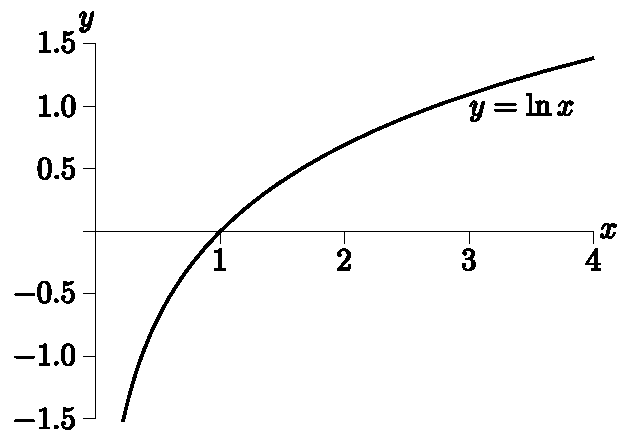
\includegraphics{logGraph}
\end{center}
\end{fig}


To compute the derivative of $\log x$ we could attempt to start with the limit
definition of the derivative
\begin{align*}
  \diff{}{x}\log x &= \lim_{h \to 0} \frac{\log(x+h) - \log(x)}{h}\\
  &= \lim_{h\to 0} \frac{\log( (x+h)/x )}{h} \\
  &= \text{um\dots}
\end{align*}
This doesn't look good. But all is not lost --- we have the chain rule, and we
know that the logarithm satisfies the equation:
\begin{align*}
  x &= e^{\log x}
\end{align*}
Since both sides of the equation are the same function, both sides of the equation
have the same derivative. i.e. we are using\footnote{Notice that just because the
derivatives are the same, doesn't mean the original functions are the same.
Both $f(x)=x^2$ and $g(x)=x^2+3$ have derivative $f'(x)=g'(x)=2x$, but $f(x)
\neq g(x)$. }
\begin{align*}
  \text{ if } f(x)=g(x) \text{ for all $x$, then } f'(x) = g'(x)
\end{align*}
So now differentiate both sides:
\begin{align*}
  \diff{}{x} x &= \diff{}{x} e^{\log x}
\intertext{The left-hand side is easy, and the right-hand side we can process
using the chain rule with $f(u)=e^u$ and $u=\log x$. }
  1 &= \diff{f}{u} \cdot \diff{u}{x} \\
  &= e^u \cdot
\underbrace{\diff{}{x} \log x }_\text{what we want to compute}\\
 \intertext{Recall that $e^u = e^{\log x} = x$, so}
 1 &= x \cdot
\underbrace{\diff{}{x} \log x }_\text{now what?}
\intertext{We can now just rearrange this equation to make the thing we want
the subject:}
 \diff{}{x} \log x &= \frac{1}{x}
\end{align*}

Thus we have proved:
\begin{theorem}\label{thm diff log}
\begin{align*}
  \diff{}{x} \log x &= \frac{1}{x}
\end{align*}
where $\log x$ is the logarithm base $e$.
\end{theorem}

\begin{eg}\label{eg_2_10_1}
 Let $f(x) = \log 3x$. Find $f'(x)$.

There are two ways to approach this --- we can simplify then differentiate, or
differentiate and then simplify. Neither is difficult.
\begin{itemize}
 \item Simplify and then differentiate:
  \begin{align*}
  f(x) &= \log 3x & \text{log of a product} \\
  &= \log 3 + \log x \\
  f'(x) &= \diff{}{x} \log 3 + \diff{}{x} \log x \\
  &= \frac{1}{x}.
\end{align*}
\item Differentiation and then simplify:
  \begin{align*}
  f'(x) &= \diff{}{x} \log(3x) & \text{chain rule} \\
  &= \frac{1}{3x} \cdot 3 \\
  &= \frac{1}{x}
\end{align*}
\end{itemize}
\end{eg}
\begin{eg}[The derivative of $\log cx$]\label{eg_2_10_2}
Notice that we can extend the previous example for any positive constant --- not
just 3. Let $c>0$ be a constant, then
\begin{align*}
  \diff{}{x} \log cx &= \diff{}{x}\left(\log c + \log x \right)\\
  &= \frac{1}{x}
\end{align*}
\end{eg}
\begin{eg}[The derivative of $\log|x|$]\label{eg diff log abs x}
 We can push this further still. Let $g(x) = \log | x |$, then\footnote{It's
probably a good moment to go back and look at Example~\ref{eg diff abs}.}
\begin{itemize}
 \item If $x>0$, $|x|= x$ and so
\begin{align*}
  g'(x) &= \diff{}{x} \log x = \frac{1}{x}
\end{align*}
\item If $x<0$ then $|x|= -x$. If $|h|$ is strictly smaller than $|x|$, 
then we also have  that $x+h<0$ and $|x+h|=-(x+h)=|x|-h$. 
Write $X=|x|$ and $H=-h$. Then, by the definition of the derivative,
\begin{align*}
  g'(x) &= \lim_{h\rightarrow 0} \frac{\log|x+h|-\log|x|}{h}
        = \lim_{h\rightarrow 0} \frac{\log(|x|-h)-\log|x|}{h} \\
        &= \lim_{H\rightarrow 0} \frac{\log(X+H)-\log X}{-H}
        = -\lim_{H\rightarrow 0} \frac{\log(X+H)-\log X}{H} \\
        &=-\diff{}{X}\log X =-\frac{1}{X} = -\frac{1}{|x|} \\
        &=\frac{1}{x}
\end{align*}
\item Since $\log 0$ is undefined, $g'(0)$ does not exist.
\end{itemize}
Putting this together gives:
\begin{align*}
  \diff{}{x} \log | x | &= \frac{1}{x}
\end{align*}
\end{eg}

\begin{eg}[The derivative of $x^a$]\label{eg diff power}
Just after Corollary \ref{cor:DIFFxtoa}, we said that we would, in the future, find the derivative of $x^a$ for all real numbers. The future is here. 
Let $x>0$ and $a$ be any real number. Exponentiating both sides of 
$\log\big(x^a\big)=a\log x$ gives us $x^a=e^{a\log x}$ and then
\begin{align*}
  \diff{}{x} x^a &= \diff{}{x} e^{a\log x}
                  = e^{a\log x} \diff{}{x}(a\log x) &\text{by the chain rule} \\
                 &=\frac{a}{x} e^{a\log x}
                  =\frac{a}{x} x^a \\
                 &=a x^{a-1}
\end{align*}
as expected.
\end{eg}




We can extend Theorem~\ref{thm diff log} to compute the derivative of
logarithms of other bases in a straightforward way. Since for any positive $a
\neq 1$:
\begin{align*}
  \log_a x &= \frac{\log x}{\log a} = \frac{1}{\log a} \cdot \log x &
\text{since $a$ is a constant}\\
  \diff{}{x} \log_a x &= \frac{1}{\log a} \cdot \frac{1}{x}
\end{align*}

\subsection*{Back to $\mathbf{\diff{}{x} a^x}$}

We can also now finally get around to computing the derivative of $a^x$ (which
we started to do back in Section~\ref{sec exp func}).
\begin{align*}
  f(x) &= a^x & \text{take log of both sides}\\
  \log f(x) &= x \log a & \text{exponentiate both sides base $e$}\\
  f(x) &= e^{x \log a} & \text{chain rule}\\
  f'(x) &= e^{x \log a} \cdot \log a \\
  &= a^x \cdot \log a
\end{align*}
Notice that we could have also done the following:
\begin{align*}
  f(x) &= a^x & \text{take log of both sides} \\
  \log f(x) &= x \log a & \text{differentiate both sides}\\
  \diff{}{x} \left( \log f(x) \right) &=
\log a \\
\intertext{We then process the left-hand side using the chain rule}
  f'(x) \cdot \frac{1}{f(x)} &= \log a \\
  f'(x) &= f(x) \cdot \log a = a^x \cdot \log a
\end{align*}
We will see $\diff{}{x} \log f(x)$ more below in the subsection on
``logarithmic differentiation''.

To summarise the results above:
\begin{cor}\label{cor_2_10}
\begin{align*}
  \diff{}{x} a^x &= \log a \cdot a^x & \text{for any $a>0$}\\
  \diff{}{x} \log_a x &= \frac{1}{x \cdot \log a} & \text{for any $a>0,
a \neq 1$}
\end{align*}
where $\log x$ is the natural logarithm.
\end{cor}
Recall that we need the caveat $a \neq 1$ because the logarithm base 1 is not
well defined. This is because $1^x = 1$ for any $x$. We do not need a similar
caveat for the derivative of the exponential because we know (recall
Example~\ref{eg log est})
\begin{align*}
  \diff{}{x} 1^x &= \diff{}{x} 1= 0 &\text{while the above corollary tells us}\\
  &= \log 1 \cdot 1^x = 0 \cdot 1 = 0.
\end{align*}

\subsection*{Logarithmic Differentiation}
We want to go back to some previous slightly messy examples
(Examples~\ref{eg:DIFFsimpleToolsA}  and~\ref{eg:DIFFsimpleToolsNB}) and now
show you how they can be done more easily.
\begin{eg}\label{eg_2_10_3}
 Consider again the derivative of the product of 3 functions:
\begin{align*}
P(x) &= F(x) \cdot G(x) \cdot H(x)
\end{align*}
Start by taking the logarithm of both sides:
\begin{align*}
 \log P(x) &= \log \left( F(x) \cdot G(x) \cdot H(x)  \right) \\
  &= \log F(x) + \log G(x) + \log H(x)
\intertext{Notice that the product of functions on the right-hand side has
become a sum of functions. Differentiating sums is much easier than
differentiating products. So when we differentiate we have}
\diff{}{x}\log P(x)  &= \diff{}{x}\log F(x) + \diff{}{x}\log G(x) + \diff{}{x}\log H(x)
\intertext{A quick application of the chain rule shows that $\diff{}{x}\log
f(x) = f'(x) / f(x)$:}
\frac{P'(x)}{P(x)} &= \frac{F'(x)}{F(x)}+\frac{G'(x)}{G(x)}+\frac{H'(x)}{H(x)}
\intertext{Multiply through by $P(x)=F(x)G(x)H(x)$:}
P'(x) &=
\left(\frac{F'(x)}{F(x)}+\frac{G'(x)}{G(x)}+\frac{H'(x)}{H(x)}\right)\cdot
F(x)G(x)H(x)\\
  &= F'(x)G(x)H(x) + F(x)G'(x)H(x) + F(x)G(x)H'(x)
\end{align*}
which is what found in Example~\ref{eg:DIFFsimpleToolsA} by repeated
application of the product rule. The above generalises quite easily to more
than 3 functions.
\end{eg}
This same trick of ``take a logarithm and then differentiate'' --- or
logarithmic differentiation --- will work any time you have a product (or
ratio) of functions.
\begin{eg}\label{eg_2_10_4}
Let's use logarithmic differentiation on the function from
Example~\ref{eg:DIFFsimpleToolsNB}:
\begin{align*}
f(x) &=\frac{(\sqrt{x}-1)(2-x)(1-x^2)}{\sqrt{x}(3+2x)}
\end{align*}
Beware however, that we may only take the logarithm of positive numbers,
and this $f(x)$ is often negative. For example, if $1<x<2$, the factor
$(1-x^2)$ in the definition of $f(x)$ is negative while all of the other factors are positive, so that $f(x)<0$. None--the--less, we can use logarithmic
differentiation to find $f'(x)$,  by exploiting the observation that
$\diff{}{x}\log|f(x)|=\frac{f'(x)}{f(x)}$. (To see this, use the chain rule and
Example \ref{eg diff log abs x}.) So we take the logarithm of $|f(x)|$ and expand.
\begin{align*}
\log |f(x)| &= \log \frac{|\sqrt{x}-1|\,|2-x|\,|1-x^2|}{\sqrt{x}|3+2x|} \\
  &= \log|\sqrt{x}-1| + \log|2-x| + \log|1-x^2| -
\underbrace{\log(\sqrt{x})}_{=\frac{1}{2}\log x} - \log|3+2x| \\
  %
\intertext{Now we can essentially just differentiate term-by-term:}
\diff{}{x}\log |f(x)| &= \diff{}{x} \left(
  \log|\sqrt{x}-1| + \log|2-x| + \log|1-x^2| - \frac{1}{2}\log(x) - \log|3+2x|
 \right)\\
\frac{f'(x)}{f(x)} &= \frac{1/(2\sqrt{x})}{\sqrt{x}-1}
  + \frac{-1}{2-x} + \frac{-2x}{1-x^2} - \frac{1}{2x} - \frac{2}{3+2x} \\
f'(x) &= f(x) \cdot \left( \frac{1}{2 \sqrt{x} (\sqrt{x}-1)}
  - \frac{1}{2-x} - \frac{2x}{1-x^2} - \frac{1}{2x} - \frac{2}{3+2x}
\right)\\
  &= \frac{(\sqrt{x}-1)(2-x)(1-x^2)}{\sqrt{x}(3+2x)}
  \cdot \left( \frac{1}{2 \sqrt{x} (\sqrt{x}-1)}
  - \frac{1}{2-x} - \frac{2x}{1-x^2} - \frac{1}{2x} - \frac{2}{3+2x}
\right)
\end{align*}
just as we found previously.
\end{eg}


%%%%%%%%%%%%%%%%%%%%%%%%%%%%%%%
\section{Implicit Differentiation}\label{sec_2_11}
%%%%%%%%%%%%%%%%%%%%%%%%%%%%%%%


Implicit differentiation is a simple trick that is used to
compute derivatives of functions either
\begin{itemize}
\item when you don't know an explicit formula for the function, but you
know an equation that the function obeys or

\item even when you have an explicit, but complicated, formula for the
function, and the function obeys a simple equation.
\end{itemize}
The trick is just to differentiate both sides of the equation and
then solve for the derivative we are seeking. In fact we have already done
this, without using the name ``implicit differentiation'', when we found the
derivative of $\log x$ in the previous section. There we knew that the function
$f(x)=\log x$ satisfied the equation $e^{f(x)}=x$ for all $x$. That is, the
functions $e^{f(x)}$ and $x$ are in fact the same function and so have the same
derivative. So we had
\begin{align*}
\diff{}{x}e^{f(x)} = \diff{}{x}x = 1
\end{align*}
We then used the chain rule to get $\diff{}{x}e^{f(x)}=e^{f(x)}f'(x)$,
which told us that $f'(x)$ obeys the equation
\begin{align*}
e^{f(x)}f'(x) &=1 & \text{and we can now solve for $f'(x)$}\\
f'(x) &= e^{-f(x)} = e^{-\log x} = \frac{1}{x}.
\end{align*}

The typical way to get used to implicit differentiation is to play with
problems involving tangent lines to curves. So here are a few examples
finding the equations of tangent lines to curves. Recall, from Theorem
\ref{thm:DIFFtangentLine}, that, in general, the tangent line to the curve
$y=f(x)$ at $\big(x_0,y_0\big)$ is $y=f(x_0)+f'(x_0)(x-x_0)=y_0+f'(x_0)(x-x_0)$.


\begin{eg}\label{eg:DIFFimpldiffD}
 Find the equation of the tangent line to $y=y^3+xy+x^3$ at $x=1$.

This is a very standard sounding example, but made a little complicated by the fact that
the curve is given by a cubic equation --- which means we cannot solve directly for $y$ in
terms of $x$ or vice versa. So we really do need implicit differentiation.
\begin{itemize}
 \item First notice that when $x=1$ the equation, $y=y^3+xy+x^3$, of the curve
simplifies to $y=y^3+y+1$ or $y^3=-1$, which we can solve\footnote{
This type of luck rarely happens in the ``real world''. But it happens
remarkably frequently in textbooks, problem sets and tests.}: $y=-1$.
So we know that the curve passes through $(1,-1)$ when $x=1$.

\item Now, to find the  slope of the tangent line at $(1,-1)$, pretend that our
curve is $y=f(x)$ so that $f(x)$ obeys
\begin{align*}
f(x) &= f(x)^3 + x f(x) + x^3
\end{align*}
for all $x$. Differentiating both sides gives
\begin{align*}
f'(x)=3f(x)^2f'(x)+f(x)+xf'(x)+3x^2
\end{align*}
\item At this point we could isolate for $f'(x)$ and write it in terms of $f(x)$
and $x$, but since we only want answers when $x=1$, let us substitute in $x=1$
and $f(1)=-1$ (since the curve passes through $(1,-1)$) and clean things up
before doing anything else.

\item Subbing in $x=1,\ f(1)=-1$ gives
\begin{align*}
f'(1)&=3f'(1)-1+f'(1)+3 & \text{ and so } f'(1)=-\frac{2}{3}
\end{align*}
\item The equation of the tangent line is
\begin{align*}
y=y_0+f'(x_0)(x-x_0)=-1-\frac{2}{3}(x-1)
=-\frac{2}{3}x-\frac{1}{3}
\end{align*}
\end{itemize}
We can further clean up the equation of the line to write it as $2x+3y=-1$.
\end{eg}
In the previous example we replace $y$ by $f(x)$ in the middle of the
computation. We don't actually have to do this. When we are writing out our
solution we can remember that $y$ is a function of $x$. So we can start with
\begin{align*}
  y &=y^3+xy+x^3 & \intertext{ and differentiate remembering that $y\equiv
y(x)$}
  y' &= 3 y^2 y' + xy' + y + 3x^2
\intertext{And now substitute $x=1, y=-1$ to get}
  y'(1) &= 3 \cdot y'(1) + y'(1) - 1 + 3 & \text{and so}\\
  y'(1) &= -\frac{2}{3}
\end{align*}


The next one is at the same time a bit easier (because it is a quadratic) and a
bit harder (because we are asked for the tangent at a general point on the curve, not a
specific one).
\begin{eg}\label{eg:DIFFimpldiffA}
Let $(x_0,y_0)$ be a point on the ellipse $3x^2+5y^2=7$. Find the equation for
the tangent lines when $x=1$ and $y$ is positive. Then find an equation
for the tangent line to the ellipse at a general point $(x_0,y_0)$.

Since we are not given an specific point $x_0$ we are going to have to be
careful with the second half of this question.
\begin{itemize}
 \item When $x=1$ the equation simplifies to
\begin{align*}
  3 + 5y^2 &= 7 \\
  5y^2 &= 4 \\
  y &= \pm \frac{2}{\sqrt{5}}.
\end{align*}
We are only interested in positive $y$, so our point on the curve
is $(1,2/\sqrt{5})$.

\item Now we use implicit differentiation to find $\diff{y}{x}$ at
this point. First we pretend that we have solved the curve explicitly, for some interval
of $x$'s, as $y=f(x)$. The equation becomes
\begin{align*}
  3x^2 + 5f(x)^2 &= 7 & \text{now differentiate} \\
  6x + 10 f(x) f'(x) &= 0 \\
  f'(x) &= - \frac{3x}{5f(x)}
\end{align*}

\item When $x=1, y= 2/\sqrt{5}$ this becomes
\begin{align*}
  f'(1) &= - \frac{3}{5 \cdot 2/\sqrt{5}} = - \frac{3}{2\sqrt{5}}
\end{align*}
So the tangent line passes through $(1,2/\sqrt{5})$ and has slope $-
\frac{3}{2\sqrt{5}}$. Hence the tangent line has equation
\begin{align*}
  y &=y_0+f'(x_0)(x-x_0) \\
    &= \frac{2}{\sqrt{5}} - \frac{3}{2\sqrt{5}} (x-1) \\
  &= \frac{7 - 3x}{2\sqrt{5}} & \text{or equivalently} \\
  3x + 2\sqrt{5} y&= 7
\end{align*}
\end{itemize}

Now we should go back and do the same but for a general point on the curve
$(x_0,y_0)$:
\begin{itemize}
  \item A good first step here is to sketch the curve. Since this is an
ellipse, it is pretty straight-forward.
\vadjust{
\begin{efig}
  \begin{center}
  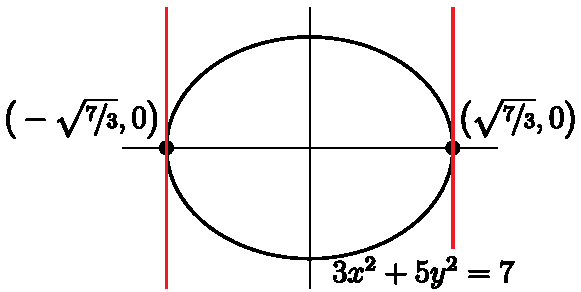
\includegraphics[scale=0.95]{ellipse}\quad
           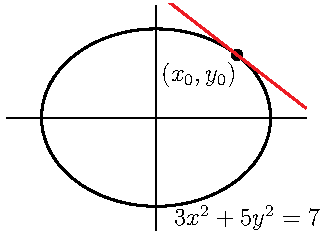
\includegraphics[scale=0.95]{ellipseB.pdf}
  \end{center}
\end{efig}
}
 \item Notice that there are two points on the ellipse --- the extreme right
and left points  $(x_0,y_0)=\pm\big(\sqrt{\nicefrac{7}{3}},0\big)$ --- at
which the tangent line is vertical. In those two cases, the tangent line is
just $x=x_0$.


\item Since this is a quadratic for $y$, we could solve it explicitly to get
\begin{align*}
y &= \pm \sqrt{\frac{7-3x^2}{5}}
\end{align*}
and choose the positive or negative branch as appropriate. Then we could
differentiate to find the slope and put things together to get the tangent line.


% We can rewrite the equation of the ellipse near $(x_0,y_0)$ explicitly
% in the form $y=f(x)$  by solving the equation $3x^2+5y^2=7$
% for $y$ as a function of $x$. Then we can find the slope, $f'(x_0)$,
% of the tangent line by differentiating $f$ and evaluating the derivative
% at $x=x_0$.

But even in this relatively easy case, it is computationally cleaner,
and hence less vulnerable to mechanical errors, to use implicit
differentiation. So that's what we'll do.

\item Now we could again ``pretend'' that we have solved the equation for the
ellipse for $y=f(x)$  near $(x_0,y_0)$, but let's not do that. Instead (as we
did just before this example) just remember that when we differentiate $y$ is
really a function of $x$. So starting from
\begin{align*}
  3x^2 + 5y^2 &=7 &\text{differentiating gives}\\
  6x + 5\cdot 2y \cdot y' &= 0
\end{align*}
We can then solve this for $y'$:
\begin{align*}
  y' &= -\frac{3x}{5y}
\end{align*}
where $y'$ and $y$ are both functions of $x$.
\item Hence at the point $(x_0,y_0)$ we have
\begin{align*}
  \left. y' \right|_{(x_0,y_0)} &= -\frac{3x_0}{5y_0}
\end{align*}
This is the slope of the tangent line at $(x_0,y_0)$ and so its equation is
\begin{align*}
  y &=y_0+y' \cdot (x-x_0) \\
  &= y_0 -\frac{3x_0}{5y_0}(x-x_0)
\intertext{We can simplify this by multiplying through by $5y_0$ to get}
  5y_0 y &= 5y_0^2-3x_0x +3x_0^2
\intertext{We can clean this up more by moving all the terms that contain $x$
or $y$ to the left-hand side and everything else to the right:}
 3x_0x+5y_0y &=3x_0^2+5y_0^2
\intertext{But there is one more thing we can do, our original equation
is $3x^2+5y^2=7$ for all points on the curve, so we know that
$3x_0^2+5y_0^2=7$. This cleans up the right-hand side.}
 3x_0x+5y_0y &=7
\end{align*}
\item In deriving this formula for the tangent line
at $(x_0,y_0)$ we have assumed that $y_0\ne 0$. But in fact the final answer
happens to also work when $y_0=0$ (which means
$x_0=\pm\sqrt{\nicefrac{7}{3} }$), so that the tangent line is $x=x_0$.
\end{itemize}
We can also check that our answer for general $(x_0,y_0)$ reduces to our answer
for $x_0=1$.
\begin{itemize}
 \item When $x_0=1$ we worked out that $y_0=2/\sqrt{5}$.
\item Plugging this into our answer above gives
\begin{align*}
  3x_0x+5y_0y &=7  &\text{sub in $(x_0,y_0)=(1,2/\sqrt{5})$}:\\
  3 x + 5 \frac{2}{\sqrt{5}} y &= 7 & \text{clean up a little}\\
  3x + 2\sqrt{5} y &=7
\end{align*}
as required.
\end{itemize}

\end{eg}


\begin{eg}\label{eg:DIFFimpldiffE}
At which points does the curve  $x^2-xy+y^2=3$ cross the $x$--axis? Are the
tangent lines to the curve at those points parallel?

This is a 2 part question --- first the $x$-intercepts and then we need to
examine  tangent lines.
\begin{itemize}
 \item Finding where the curve crosses the $x$-axis is straight forward. It
does so when $y=0$. This means $x$ satisfies
\begin{align*}
  x^2-x\cdot 0+0^2&=3 & \text{ so $x = \pm\sqrt{3}$}.
\end{align*}
So the curve crosses the $x$--axis at two points $\big(\pm\sqrt{3}\,,\,0\big)$.
\item Now we need to find the tangent lines at those points. But we don't
actually need the lines, just their slopes. Again we can pretend that near one
of those points the curve is $y=f(x)$. Applying $\diff{}{x}$ to both sides of
$x^2-xf(x)+f(x)^2=3$ gives
\begin{align*}
  2x-f(x)-xf'(x)+2f(x)f'(x)&=0
\end{align*}
etc etc.

\item But let us stop ``pretending''. Just make sure we remember that $y$ is a
function of $x$ when we differentiate:
\begin{align*}
  x^2-xy+y^2 &= 3 & \text{start with the curve, and differentiate}\\
  2x - xy' -y + 2yy' &=0 &
\end{align*}
Now substitute in the first point, $x=+\sqrt{3}, y=0$:
\begin{align*}
  2\sqrt{3} - \sqrt{3}y' + 0 &=0 \\
  y' &= 2
\end{align*}
And now do the second point $x=-\sqrt{3}, y=0$:
\begin{align*}
  -2\sqrt{3} + \sqrt{3}y' + 0 &=0 \\
  y' &= 2
\end{align*}
Thus the slope is the same at $x=\sqrt{3}$ and $x=-\sqrt{3}$ and the tangent
lines are parallel.
\end{itemize}
\begin{efig}
 \begin{center}
  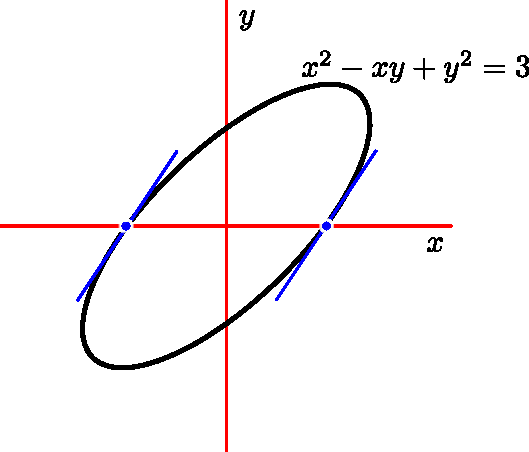
\includegraphics[height=4cm]{implicit_eg1}
 \end{center}
\end{efig}

\end{eg}

Okay --- let's get away from curves and do something a little different.

\begin{eg}\label{eg:DIFFimpldiffC}
You are standing at the origin. At time zero a pitcher throws a ball at
your head\footnote{It seems that it is not a friendly game today.}.
\begin{sfig}\label{fig:DIFFbaseball}
\begin{center}
  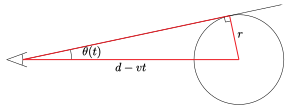
\includegraphics{baseball}
\end{center}
\end{sfig}
The position of the (centre of the) ball at time $t$ is $x(t)=d-vt$, where $d$ is
the distance from your head to the  pitcher's mound and $v$ is the ball's
velocity. Your eye sees the ball filling \footnote{This is the ``visual angle''
or ``angular size''.} an angle $2\theta(t)$ with
\begin{align*}\label{eq:DIFFbaseball}
\sin\big(\theta(t)\big)=\frac{r}{d-vt}
\end{align*}
where $r$ is the radius of the baseball. The question is ``How fast is
$\theta$ growing at time $t$?'' That is, what is $\diff{\theta}{t}$?

\begin{itemize}
 \item We don't know (yet) how to solve this equation to find
$\theta(t)$ explicitly. So we use implicit differentiation.

\item To do so we apply $\diff{}{t}$ to both sides of
our equation. This gives
\begin{align*}
\cos\big(\theta(t)\big)\cdot\theta'(t)=\frac{rv}{(d-vt)^2}
\end{align*}
\item Then we solve for $\theta'(t)$:
\begin{align*}
\theta'(t)=\frac{rv}{(d-vt)^2\cos\big(\theta(t)\big)}
\end{align*}
\item As is often the case, when using implicit differentiation, this answer
is not very satisfying because it contains $\theta(t)$, for which we still
do not have an explicit formula. However in this case we can get an
explicit formula for $\cos\big(\theta(t)\big)$, without having an explicit
formula for $\theta(t)$, just by looking at the right--angled triangle
in Figure \ref{fig:DIFFbaseball}, above.

\item The hypotenuse of that triangle has length $d-vt$. By Pythagoras, the
length of the side of the triangle adjacent of the angle $\theta(t)$ is
$\sqrt{(d-vt)^2-r^2}$. So
\begin{equation*}
\cos\big(\theta(t)\big)=\frac{\sqrt{(d-vt)^2-r^2}}{d-vt}
\end{equation*}
and
\begin{align*}
\theta'(t)=\frac{rv}{(d-vt)\sqrt{(d-vt)^2-r^2}}
\end{align*}
% \item We can simplify this a bit more with an approximation. Notice that
% the radius of the baseball is typicallythis
%
% Usually $r$, the radius of the baseball, is a lot smaller than
% $d-vt$, the distance from the baseball to your head, and then
% \begin{align*}
% \sqrt{(d-vt)^2-r^2}\approx \sqrt{(d-vt)^2}=d-vt
% \implies \theta'(t)\approx\frac{rv}{(d-vt)^2}
% \end{align*}
\end{itemize}
\end{eg}

Okay --- just one more tangent-to-the-curve example and then we'll go on to
something different.
\begin{eg}\label{eg:DIFFimpldiffB}
Let $(x_0,y_0)$ be a point on the astroid\footnote{Here is where is the
astroid comes from. Imagine two circles, one of radius $1/4$ and
one of radius $1$. Paint a red dot on the smaller circle. Then imagine
the smaller circle rolling around the inside of the larger circle. The
curve traced by the red dot is our astroid. Google ``astroid'' (be careful
about the spelling) to find animations showing this.

The astroid was first discussed by Johann Bernoulli in 1691--92. It also
appears in the work of Leibniz.}
\begin{align*}
x^{\nicefrac{2}{3}}+y^{\nicefrac{2}{3}}=1.
\end{align*}
Find an equation for the tangent line to the astroid at $(x_0,y_0)$.

\begin{itemize}
 \item As was the case in examples above we can rewrite the equation of
the astroid near $(x_0,y_0)$ in the form $y=f(x)$, with an explicit $f(x)$, by
solving the equation $x^{\nicefrac{2}{3}}+y^{\nicefrac{2}{3}}=1$. But again, it
is computationally cleaner, and hence less vulnerable to mechanical errors, to
use implicit differentiation. So that's what we'll do.

\item First up, since $(x_0,y_0)$ lies on the curve, it satisfies
\begin{align*}
x_0^{\nicefrac{2}{3}}+y_0^{\nicefrac{2}{3}}=1.
\end{align*}

\item Now, no pretending that $y=f(x)$, this time --- just make sure we
remember when we differentiate that $y$ changes with $x$.
\begin{align*}
  x^{\nicefrac{2}{3}}+y^{\nicefrac{2}{3}} &=1 &\text{start with the curve, and
differentiate}\\
\frac{2}{3}x^{-\nicefrac{1}{3}} + \frac{2}{3} y^{-\nicefrac{1}{3}} y' &=0
\end{align*}

\item Note the derivative of $x^{\nicefrac{2}{3}}$, namely
$\frac{2}{3}x^{-\nicefrac{1}{3}}$, and the derivative of
$y^{\nicefrac{2}{3}}$, namely $\frac{2}{3} y^{-\nicefrac{1}{3}}y'$,
are defined only when $x\ne 0$ and $y\ne 0$. We are interested in the case that
$x=x_0$ and $y=y_0$. So we better assume that $x_0\ne 0$ and $y_0\ne 0$.
Probably something weird happens when $x_0=0$ or $y_0=0$. We'll come back to
this shortly.

\item To continue on, we set $x=x_0, y=y_0$ in the equation above, and
then solve for $y'$:
\begin{equation*}
\frac{2}{3}x_0^{-\nicefrac{1}{3}}
+\frac{2}{3} y_0^{-\nicefrac{1}{3}} y'(x)=0
\implies y'(x_0)= -\left( \frac{y_0}{x_0} \right)^{\nicefrac{1}{3}}
\end{equation*}
This is the slope of the tangent line and its equation is
\begin{equation*}
y=y_0+f'(x_0)(x-x_0) = y_0
-\left(\frac{y_0}{x_0}\right)^{\nicefrac{1}{3}}(x-x_0)
\end{equation*}
\end{itemize}


Now let's think a little bit about what the tangent line slope of
$-\root{3}\of {\nicefrac{y_0}{x_0}}$ tells us about the astroid.
\begin{itemize}
 \item First, as a preliminary observation, note that since
$x_0^{\nicefrac{2}{3}}\ge0$ and $y_0^{\nicefrac{2}{3}}\ge0$ the equation
$x_0^{\nicefrac{2}{3}}+y_0^{\nicefrac{2}{3}}=1$ of the astroid forces
$0\le x_0^{\nicefrac{2}{3}},y_0^{\nicefrac{2}{3}} \le 1$ and
hence $-1\le x_0,y_0\le 1$.

\item For all $x_0,y_0>0$ the slope $-\root{3}\of {\nicefrac{y_0}{x_0}}
<0$. So at all points on the astroid that are in the first quadrant,
the tangent line has negative slope, i.e. is ``leaning backwards''.

\item  As $x_0$ tends to zero, $y_0$ tends to $\pm 1$ and the
tangent line slope tends to infinity. So at points on the astroid near
$(0,\pm 1)$, the tangent line is almost vertical.

\item As $y_0$ tends to zero, $x_0$ tends to $\pm 1$ and the
tangent line slope tends to zero. So at points on the astroid near
$(\pm 1,0)$, the tangent line is almost horizontal.
\end{itemize}
Here is a figure illustrating all this.
\begin{efig}
\begin{center}
   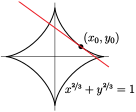
\includegraphics{astroid}\qquad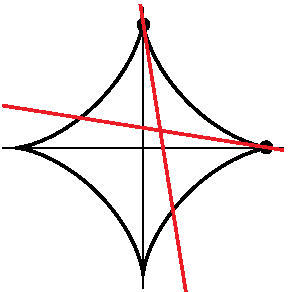
\includegraphics{astroidB}
\end{center}
\end{efig}
Sure enough, as we speculated earlier, something weird does happen
to the astroid when $x_0$ or $y_0$ is zero. The astroid is pointy,
and does not have a tangent there.
\end{eg}



\begin{comment}
%%%%%%%%%%%%%%%%%%%%%%%%%%%%%%%
\section{Inverse Functions}\label{sec:INTinverseFunctions}
%%%%%%%%%%%%%%%%%%%%%%%%%%%%%%%
In Section~\ref{sec diff logs} we

In Example \ref{eg:DIFFimpldiffC} we encountered the problem of trying
to solve the equation
\begin{align*}
\sin\big(\theta(t)\big) &=\frac{r}{d-vt} & \text{for $\theta(t)$}.
\end{align*}
for $\theta(t)$. We're now going to consider, more generally, problems in which
\begin{itemize}
\item we have a given function, that we'll call $f$, and
\item for each number $X$
\item we wish to find a number $Y$ satisfying
\begin{equation}\label{eq:DIFFinversePblm}
f(Y)=X
\end{equation}
\end{itemize}

If we're lucky, then for each real number $X$ there is exactly one
real number $Y$, that we'll call $f^{-1}(X)$,
obeying \eqref{eq:DIFFinversePblm}. Then $f^{-1}$ is called the inverse
function of $f$. A (trivial) example in which this happens is given
in Example \ref{eg:INVlucky}, below.

 If we're a little less lucky, there is a set of real numbers $\cD$
(that does not contain all of $\bbbr$) such that
\begin{itemize} \itemsep1pt \parskip0pt \parsep0pt
\item for each real number $X$ in $\cD$ there is exactly one real
number $Y$, that we'll again call $f^{-1}(X)$, obeying
\eqref{eq:DIFFinversePblm} but
\item for each real number $X$ that is \emph{not} in $\cD$ there is \emph{no}
$Y$ obeying \eqref{eq:DIFFinversePblm}.
\end{itemize}
Then $f^{-1}$ is again called the inverse function of $f$ and $\cD$
is called the domain of $f^{-1}$. We have already seen an example of this
--- namely $f(x)=e^x$. We'll review this example in Example \ref{eg:INVlesslucky}, below.

If we're still little less lucky, there is at least one real number $X$
for which there is more than one real number $Y$ obeying
\eqref{eq:DIFFinversePblm}. The trigonometric functions are like this.
We'll take a first quick look at this in  Example \ref{eg:INVstilllesslucky},
below and take a more thorough look in \S\ref{sec:invTrig}, below.


\begin{eg}\label{eg:INVlucky}
Let $f(x)=2x$. For this $f(x)$, equation \eqref{eq:DIFFinversePblm}
becomes
\begin{equation*}
2Y=X
\end{equation*}
For each real number $X$, there is exactly one $Y$, namely
$Y=\frac{X}{2}$, that obeys $2Y=X$. So, the function $f(x)=2x$
has inverse function $f^{-1}(X) =\frac{X}{2}$.

\end{eg}


\begin{eg}\label{eg:INVlesslucky}
Let $f(x)=e^x$. For this $f(x)$, equation \eqref{eq:DIFFinversePblm}
becomes
\begin{equation*}
e^Y=X
\end{equation*}
For concreteness, let's pick a specific value of $X$, say $X=2$.
The graph of $e^Y$, as a function of $Y$, is sketched below. In that
sketch, the $x$--axis has been renamed the $Y$--axis, because we are interested
in $e^Y$ as a function of $Y$. (Be careful to distinguish the upper
case $Y$ from the lower case $y$.)
\vadjust{
\begin{efig}
\begin{center}
  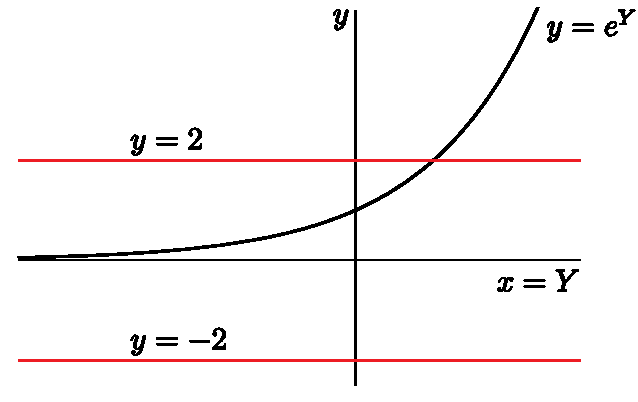
\includegraphics{expInv}
\end{center}
\end{efig}
}
The number of $Y$'s obeying $e^Y=2$ is exactly the number of times
the horizontal straight line $y=2$ intersects the graph $y=e^Y$, which is
one. So for $X=2$, there is exactly one $Y$ obeying $e^Y=X$.
On the other hand, for $X=-2$, the number of $Y$'s obeying $e^Y=-2$
is exactly the number of times the horizontal straight line $y=-2$
intersects the graph $y=e^Y$, which is zero. So for $X=-2$,
no $Y$'s obey $e^Y=X$.

As $Y$ runs from $-\infty$ to $+\infty$, $e^Y$ takes each strictly
positive value exactly once and never takes any value zero or smaller.
So the domain of $\ln x$, the inverse function of $e^x$, is exactly
the interval $(0,\infty)$.


\end{eg}


\begin{eg}\label{eg:INVstilllesslucky}
Let $f(x)=\sin(x)$. For this $f(x)$, equation \eqref{eq:DIFFinversePblm}
becomes
\begin{equation*}
\sin(Y)=X
\end{equation*}
For each fixed real number $X$, the number of $Y$'s that obey
$\sin(Y)=X$, is exactly the number of times the horizontal straight line
$y=X$ intersects the graph $y=\sin(Y)$. When $-1\le X\le 1$, the line
$y=X$ intersects the graph $y=\sin(Y)$ infinitely many times. This is
illustrated in the figure below by the line $y=0.3$. On the other
hand, when $X<-1$ or $X>1$, the line $y=X$ never intersects the graph
$y=\sin(Y)$. This is illustrated in the figure below by the line
$y=-1.2$. We'll see what is normally done about this in \S\ref{sec:invTrig},
below.

\begin{efig}
\begin{center}
  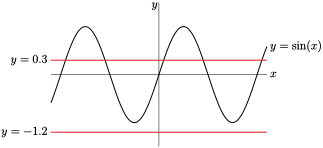
\includegraphics{sinInv}
\end{center}
\end{efig}

\end{eg}

It is an easy matter to construct the graph of an inverse function
from the graph of the original function. We just need to remember that
\begin{equation*}
Y=f^{-1}(X)  \iff f(Y)=X
\end{equation*}
which is $y=f(x)$ with $x$ renamed to $Y$ and $y$ renamed to $X$.
%Each point on the graph of $f$ has coordinates $\big(x\,,\,f(x)\big)$.
%If we rename $x$ to $Y$, those coordinates become
%\begin{equation*}
%\big(Y,f(Y)\big) = \big(f^{-1}(X),X\big) = (Y,X)\quad\text{with}\quad Y=f^{-1}(X)
%\end{equation*}
%To get the graph of $f^{-1}$ we just need to reinterpret these statements
%graphically.

 Start by drawing the graph of $f$, labelling the $x$-- and $y$--axes
and labelling the curve $y=f(x)$.
\begin{efig}
\begin{center}
   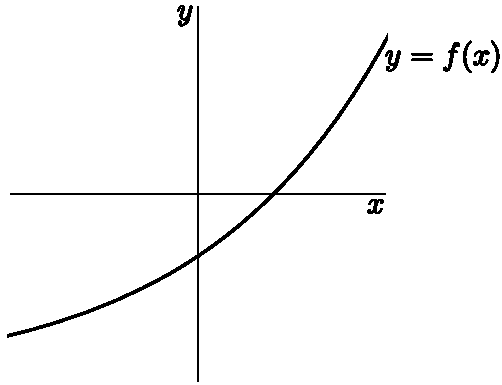
\includegraphics{fInvA}
\end{center}
\end{efig}
Now replace each $x$ by $Y$ and each $y$ by $X$  and replace the resulting
label $X=f(Y)$ on the curve by the equivalent $Y=f^{-1}(X)$.
\begin{efig}
\begin{center}
   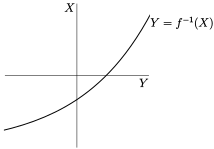
\includegraphics{fInvB}
\end{center}
\end{efig}
Finally we just need to redraw the sketch with the $Y$ axis running vertically
(with $Y$ increasing upwards) and the $X$ axis running horizontally (with
$X$ increasing to the right). To do so, pretend that the sketch was on
a transparency or on a very thin piece of paper that you can see through.
Lift the sketch up and flip it over so that the $Y$ axis runs vertically
and the $X$ axis runs horizontally. If you want can also convert the upper
case $X$ into a lower case $x$ and the upper case $Y$ into a lower case
$y$.
\begin{wfig}
\begin{center}
   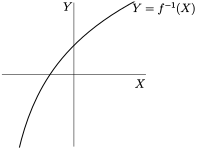
\includegraphics{fInvC}\qquad   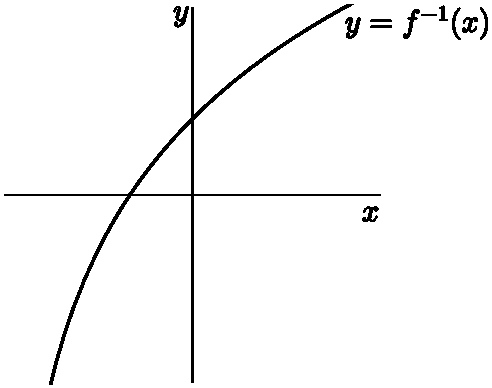
\includegraphics{fInvD}
\end{center}
\end{wfig}

It is also an easy matter to use implicit differentiation to find
a formula for the derivative\footnote{There is a theorem called the
Inverse Function Theorem, which we will not prove, that says that,
under reasonable hypotheses on $f(x)$,
$f^{-1}(x)$ is differentiable.} of $f^{-1}$ in terms of the derivative of
$f$. Substitute $Y=f^{-1}(X)$ into $f(Y)=X$ to give
\begin{equation*}
f\big(f^{-1}(X)\big)=X
\end{equation*}
Rename $X$ to $x$ and apply $\diff{}{x}$ to both sides.
\begin{equation*}
\diff{}{x}f\big(f^{-1}(x)\big)=\diff{}{x}x=1
\end{equation*}
By the chain rule
\begin{equation}\label{eq:DIFFinvderiv}
f'\big(f^{-1}(x)\big)\cdot \diff{}{x} f^{-1}(x)=1
\implies  \diff{}{x} f^{-1}(x) = \frac{1}{f'\big(f^{-1}(x)\big)}
\end{equation}

\begin{eg}\label{eg:DIFFlnderiv}
The inverse function of $f(x)=e^x$ is $f^{-1}(x)=\ln x$. Since $f'(x)=e^x$,
\eqref{eq:DIFFinvderiv} gives
\begin{equation*}
\diff{}{x} \ln x = \frac{1}{e^{\ln x}}=\frac{1}{x}
\end{equation*}
This is of course the same answer for $\diff{}{x} \ln x$ as we saw in
\eqref{eq:DIFFdln}. (In fact \eqref{eq:DIFFdln} was exactly the computation
of \eqref{eq:DIFFinvderiv} in the special case that $f(x)=e^x$.)
\end{eg}
\end{comment}


%%%%%%%%%%%%%%%%%%%%%%%%%%%%%%%%%%%%%%%%%%
\section{Inverse Trigonometric Functions}\label{sec:invTrig}
%%%%%%%%%%%%%%%%%%%%%%%%%%%%%%%%%%%%%%%%%%
One very useful application of implicit differentiation is to find the
derivatives of inverse functions. We have already used this approach to find
the derivative of the inverse of the exponential function --- the
logarithm.

We are now going to consider the problem of finding the derivatives of the
inverses of trigonometric functions. Now is a very good time to go back
and reread Section~\ref{sec inverse functions} on inverse functions ---
especially Definition~\ref{def inv func}. Most importantly, given a function $f(x)$, its
inverse function $f^{-1}(x)$ only exists, with domain $D$, when $f(x)$ passes the
``horizontal line test'', which says that for each $Y$ in $D$ the horizontal line $y=Y$
intersects the graph $y=f(x)$ exactly once. (That is, $f(x)$  is a one-to-one function.)

Let us start by playing with the sine function and determine how to restrict
the domain of $\sin x$ so that its inverse function exists.
\begin{eg}\label{eg:INVstilllesslucky}
Let $y=f(x)=\sin(x)$. We would like to find the inverse function which takes
$y$ and returns to us a unique $x$-value so that $\sin(x)=y$.
\begin{efig}
\begin{center}
  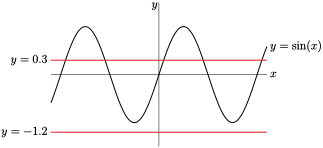
\includegraphics{sinInv}
\end{center}
\end{efig}
\begin{itemize}
 \item For each real number $Y$, the number of $x$-values that obey
$\sin(x)=Y$, is exactly the number of times the horizontal straight line
$y=Y$ intersects the graph of $\sin(x)$.
\item When $-1\le Y\le 1$, the horizontal line intersects the graph infinitely many
times. This is illustrated in the figure above by the line $y=0.3$.
\item On the other hand, when $Y<-1$ or $Y>1$, the line $y=Y$ never
intersects the graph of $\sin(x)$. This is illustrated in the figure above by
the line $y=-1.2$.
\end{itemize}
This is exactly the horizontal line test and it shows that the sine function is
not one-to-one.

Now consider the function
\begin{align*}
  y &= \sin(x) & \text{with domain } -\frac{\pi}{2} \leq x \leq \frac{\pi}{2}
\end{align*}
This function has the same formula but the domain has been restricted so that, as we'll
now show, the horizontal line test is satisfied.
\begin{efig}
\begin{center}
  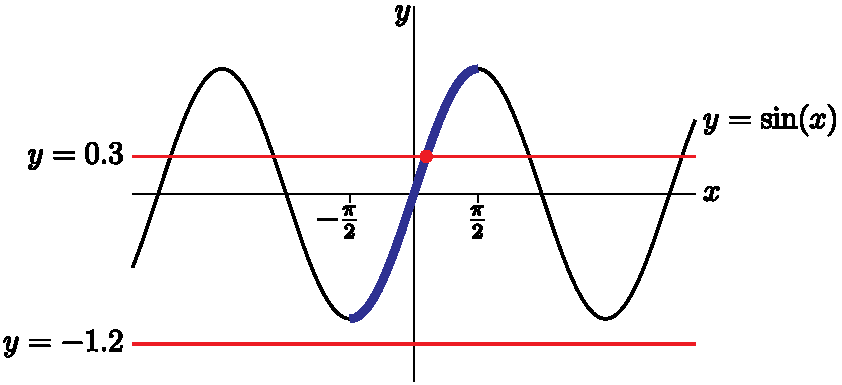
\includegraphics{sinInvB}
\end{center}
\end{efig}
As we saw above when $|Y|>1$ no $x$ obeys $\sin(x)=Y$ and, for each $-1\le Y\le 1$,
the line $y=Y$ (illustrated in the figure above with $y=0.3$) crosses the
curve $y=\sin(x)$ infinitely many times, so that there are infinitely
many $x$'s that obey $f(x)=\sin x=Y$. However exactly one of those crossings
(the dot in the figure) has $-\nicefrac{\pi}{2}\le x \le\nicefrac{\pi}{2}$.

That is, for each $-1\le Y \le 1$, there is exactly one $x$, call it $X$, that obeys both
\begin{align*}
      \sin X &= Y &\text{and} && -\frac{\pi}{2}\le X \le \frac{\pi}{2}
\end{align*}
That unique value, $X$, is typically denoted $\arcsin(Y)$. That is
\begin{align*}
  \sin( \arcsin(Y) ) &= Y & \text{and} && -\frac{\pi}{2}\le \arcsin(Y) \le\frac{\pi}{2}
\end{align*}
Renaming $Y\rightarrow x$, the inverse function $\arcsin(x)$ is
defined for all $-1 \le x \le 1$ and is determined by the
equation
\begin{equation}\label{eq:DIFFarcsin}
\sin\big(\arcsin(x)\big)=x\qquad\text{and}\qquad
        -\frac{\pi}{2}\le \arcsin(x)\le\frac{\pi}{2}.
\end{equation}
Note that many texts will use $\sin^{-1}(x)$ to denote arcsine, however we will use
$\arcsin(x)$ since we feel that it is clearer\footnote{The main reason being that people
frequently confuse $\sin^{-1}(x)$ with $(\sin(x))^{-1} = \frac{1}{\sin x}$. We feel that
prepending the prefix ``arc'' less likely to lead to such confusion. The notations
$\textrm{asin}(x)$ and $\textrm{Arcsin}(x)$ are also used.}; the reader should recognise
both.


\end{eg}


\begin{eg}\label{eg:DIFFinvsin}
Since
\begin{equation*}
\sin\frac{\pi}{2}=1\qquad\sin\frac{\pi}{6}=\frac{1}{2}
\end{equation*}
and $-\nicefrac{\pi}{2}\le \nicefrac{\pi}{6},\nicefrac{\pi}{2}\le \nicefrac{\pi}{2}$,
we have
\begin{equation*}
\arcsin 1=  \frac{\pi}{2}\qquad \arcsin \frac{1}{2}=  \frac{\pi}{6}
\end{equation*}
Even though
\begin{equation*}
\sin(2\pi)=0
\end{equation*}
it is \textbf{not} true that $\arcsin 0 =2\pi$, and it is \textbf{not}
true that $\arcsin\big(\sin(2\pi)\big) =2\pi$, because $2\pi$ is not
between $-\nicefrac{\pi}{2}$ and $\nicefrac{\pi}{2}$. More generally
\begin{align*}
\arcsin\big(\sin(x)\big) &=\text{ the unique angle $\theta$ between
$-\nicefrac{\pi}{2}$ and $\nicefrac{\pi}{2}$ obeying $\sin \theta =\sin x$} \\
&= x\quad\text{if and only if $-\nicefrac{\pi}{2}\le x\le \nicefrac{\pi}{2}$}
\end{align*}
So, for example, $\arcsin\big(\sin\big(\nicefrac{11\pi}{16}\big)\big)$
cannot be $\nicefrac{11\pi}{16}$ because $\nicefrac{11\pi}{16}$ is
bigger than $\nicefrac{\pi}{2}$. So how do we find the correct answer?
Start by sketching the graph of $\sin(x)$.
\begin{efig}
\begin{center}
  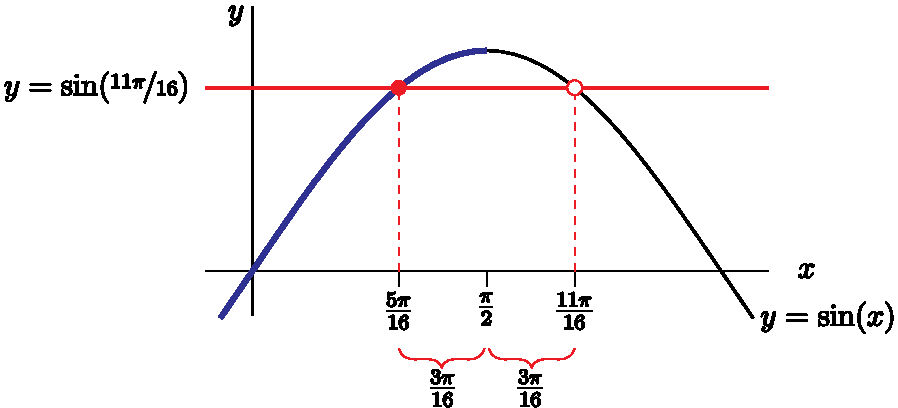
\includegraphics{sinInvEg}
\end{center}
\end{efig}
It looks like the graph of $\sin x$ is symmetric about $x=\nicefrac{\pi}{2}$.
The mathematical way to say that ``the graph of $\sin x$ is symmetric about
$x=\nicefrac{\pi}{2}$'' is ``$\sin(\nicefrac{\pi}{2}-\theta)=
\sin(\nicefrac{\pi}{2}+\theta)$'' for all $\theta$. That is indeed true\footnote{Indeed
both are equal to $\cos \theta$. You can see this by playing with the trig identities in
Appendix~\ref{sec trig add}.}.


Now $\nicefrac{11\pi}{16}=\nicefrac{\pi}{2} +\nicefrac{3\pi}{16}$ so
\begin{equation*}
\sin\Big(\frac{11\pi}{16}\Big)
=\sin\Big(\frac{\pi}{2}+\frac{3\pi}{16}\Big)
=\sin\Big(\frac{\pi}{2}-\frac{3\pi}{16}\Big)
=\sin\Big(\frac{5\pi}{16}\Big)
\end{equation*}
and, since $\nicefrac{5\pi}{16}$ is indeed between $-\nicefrac{\pi}{2}$ and
$\nicefrac{\pi}{2}$,
\begin{equation*}
\arcsin\Big(\sin\Big(\frac{11\pi}{16}\Big)\Big)
=\frac{5\pi}{16}\qquad\Big(\text{and \textbf{not} $\frac{11\pi}{16}$}\Big).
\end{equation*}

\end{eg}

\subsection*{Derivatives of Inverse Trig Functions}
Now that we have explored the arcsine function we are ready to find its derivative.
Lets call
\begin{align*}
  \arcsin(x) &= \theta(x),
\end{align*}
so that the derivative we are seeking is $\diff{\theta}{x}$. The above equation is (after
taking sine of both sides) equivalent to
\begin{align*}
  \sin(\theta) &= x
\end{align*}
Now differentiate this using implicit differentiation (we just have to remember
that $\theta$ varies with $x$ and use the chain rule carefully):
\begin{align*}
  \cos(\theta) \cdot \diff{\theta}{x} &= 1 \\
  \diff{\theta}{x} &= \frac{1}{\cos(\theta)} & \text{substitute $\theta = \arcsin x$}\\
  \diff{}{x} \arcsin x &= \frac{1}{\cos(\arcsin x)}
\end{align*}
This doesn't look too bad, but it's not really very satisfying because the right hand
side is expressed in terms of $\arcsin(x)$ and we do not have an explicit formula for
$\arcsin(x)$.

However even without an explicit formula for $\arcsin(x)$, it is a simple matter to get an
explicit formula for $\cos\big(\arcsin(x)\big)$, which is all we need. Just draw a
right--angled triangle with one angle being $\arcsin(x)$. This is done in the figure
below\footnote{The figure is drawn for the case that
$0\le\arcsin(x)\le\nicefrac{\pi}{2}$.
Virtually the same argument works for the case
$-\nicefrac{\pi}{2}\le\arcsin(x)\le 0$}.
\begin{efig}
\begin{center}
  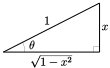
\includegraphics{triangleAsin}
\end{center}
\end{efig}
Since $\sin(\theta)=x$ (see \eqref{eq:DIFFarcsin}),
we have made the side opposite the angle $\theta$ of length $x$ and the
hypotenuse of length $1$. Then, by Pythagoras, the side adjacent to $\theta$
has length $\sqrt{1-x^2}$ and so
\begin{align*}
\cos\big(\arcsin(x)\big)=\cos(\theta)=\sqrt{1-x^2}
\end{align*}
which in turn gives us the answer we need:
\begin{align*}%\label{eq:DIFFasinDeriv}
\diff{}{x} \arcsin(x) =\frac{1}{\sqrt{1-x^2}}
\end{align*}

The definitions for $\arccos$, $\arctan$ and $\arccot$ are developed in 
the same way. Here are the graphs that are used.
\begin{efig}
\begin{center}
  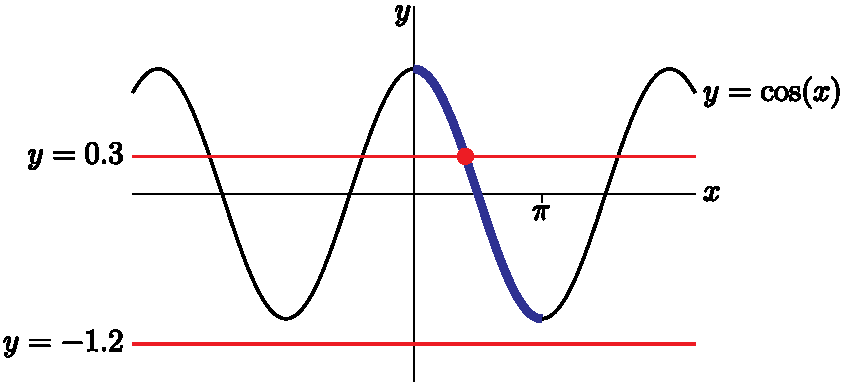
\includegraphics{cosInvB}
\end{center}
\begin{center}
  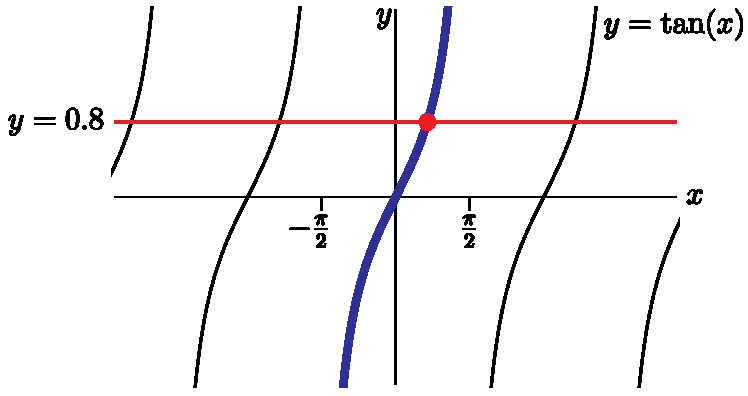
\includegraphics{tanInvB}
\end{center}
\begin{center}
  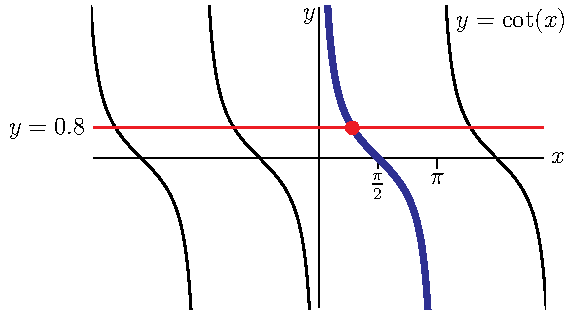
\includegraphics{cotInvB.pdf}
\end{center}
\end{efig}
The definitions for the remaining two inverse trigonometric functions
may also be developed in the same way\footnote{In fact, there are two 
different widely used definitions of $\arcsec x$. Under our definition, below, $\theta=\arcsec x$ takes values in $0\le\theta\le\pi$. Some people, 
perfectly legitimately, define $\theta=\arcsec x$ to
take values in the union of $0\le \theta<\frac{\pi}{2}$ and $\pi\le\theta<\frac{3\pi}{2}$.
Our definition is sometimes called the ``trigonometry friendly'' definition.
The definition itself has the advantage of simplicity. The other definition is sometimes called the ``calculus friendly'' definition. It eliminates some absolute values and hence simplifies some computations. Similarly, there are two different widely used definitions of $\arccsc x$.}\footnote{One could also define 
$\arccot(x)=\arctan(1/x)$ with $\arccot(0)=\frac{\pi}{2}$. We have chosen not to do so, because the definition we have chosen is both continuous and standard.}. But it's a little easier to use
\begin{align*}
\csc x=\frac{1}{\sin x} \qquad
\sec x=\frac{1}{\cos x} 
\end{align*}

\begin{defn}\label{def:DIFFinvtrig}
$\arcsin x$ is defined for $|x|\le 1$. It is the unique number obeying
\begin{align*}
\sin\big(\arcsin(x)\big)&=x &&\text{and}&
        -\frac{\pi}{2}\le &\arcsin(x)\le\frac{\pi}{2}
\intertext{
    $\arccos x$ is defined for $|x|\le 1$. It is the unique number obeying
         }
\cos\big(\arccos(x)\big)&=x &&\text{and}&
        0\le &\arccos(x)\le\pi
\intertext{
    $\arctan x$ is defined for all $x\in\bbbr$. It is the unique number obeying
         }
\tan\big(\arctan(x)\big)&=x &&\text{and}&
        -\frac{\pi}{2}< &\arctan(x)<\frac{\pi}{2}
\intertext{
    $\arccsc x=\arcsin\frac{1}{x}$ is defined for $|x|\ge 1$. It is the
unique number obeying
         }
\csc\big(\arccsc(x)\big)&=x &&\text{and}&
        -\frac{\pi}{2}\le &\arccsc(x)\le\frac{\pi}{2}
\intertext{\ \ \ \ \ \ \ \ Because $\csc(0)$ is undefined, $\arccsc(x)$ never takes the value $0$.}
\intertext{
    $\arcsec x=\arccos\frac{1}{x}$ is defined for $|x|\ge 1$. It is the
unique number obeying
         }
\sec\big(\arcsec(x)\big)&=x &&\text{and}&
        0\le &\arcsec(x)\le\pi
\intertext{\ \ \ \ \ \ \ \  Because $\sec(\pi/2)$ is undefined, $\arcsec(x)$ never takes the value $\pi/2$.}
\intertext{
    $\arccot x$ is defined for all $x\in\bbbr$. It
is the unique number obeying
         }
\cot\big(\arccot(x)\big)&=x &&\text{and}&
        0< &\arccot(x) <\pi
\end{align*}
\end{defn}

\begin{eg}\label{eg_2_12_1}
To find the derivative of $\arccos$ we can follow the same steps:
\begin{itemize}
 \item Write $\arccos(x) =\theta(x)$ so that $\cos\theta = x$ and the desired
derivative is $\diff{\theta}{x}$.
\item Differentiate implicitly, remembering that $\theta$ is a function of $x$:
  \begin{align*}
  -\sin\theta \diff{\theta}{x} &= 1 \\
  \diff{\theta}{x} &= -\frac{1}{\sin\theta} \\
  \diff{}{x}\arccos x &= -\frac{1}{\sin(\arccos x)}.
\end{align*}
\item To simplify this expression, again draw the relevant triangle
\begin{efig}
\begin{center}
  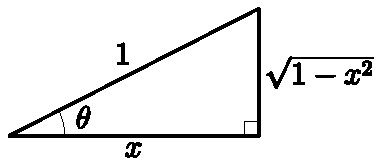
\includegraphics{triangleAcos}
\end{center}
\end{efig}
from which we see
\begin{align*}
\sin(\arccos x) = \sin\theta &= \sqrt{1-x^2}.
\end{align*}
\item Thus
\begin{align*}
  \diff{}{x}\arccos x &= -\frac{1}{\sqrt{1-x^2}}.
\end{align*}
\end{itemize}
\end{eg}

\begin{eg}\label{eg_2_12_2}
Very similar steps give the derivative of $\arctan x$:
\begin{itemize}
 \item Start with $\theta = \arctan x$, so $\tan \theta = x$.
\item Differentiate implicitly:
  \begin{align*}
  \sec^2 \theta \diff{\theta}{x} &= 1 \\
  \diff{\theta}{x} &= \frac{1}{\sec^2 \theta} = \cos^2 \theta\\
  \diff{}{x}\arctan x &= \cos^2(\arctan x).
\end{align*}
\item To simplify this expression, we draw the relevant triangle
\begin{efig}
\begin{center}
  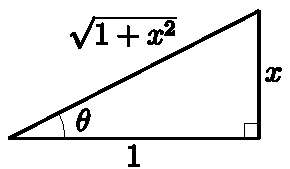
\includegraphics{triangleAtan}
\end{center}
\end{efig}
from which we see
\begin{align*}
\cos^2(\arctan x) = \cos^2\theta = \frac{1}{1+x^2}
\end{align*}
\item Thus
\begin{align*}
  \diff{}{x}\arctan x &= \frac{1}{1+x^2}.
\end{align*}
\end{itemize}
An almost identical computation gives the derivative of $\arccot x$:
\begin{itemize}
 \item Start with $\theta = \arccot x$, so $\cot \theta = x$.
\item Differentiate implicitly:
  \begin{align*}
  -\csc^2 \theta \diff{\theta}{x} &= 1 \\
\diff{}{x}\arccot x =
  \diff{\theta}{x} &= -\frac{1}{\csc^2 \theta} = -\sin^2 \theta
                      =-\frac{1}{1+x^2}
\end{align*}
 from the triangle
\begin{efig}
\begin{center}
  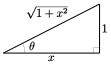
\includegraphics{triangleAcot}
\end{center}
\end{efig}
\end{itemize}
\end{eg}




\begin{eg}\label{eg_2_12_3}
 To find the derivative of $\arccsc$ we can use its definition and the chain rule.
\begin{align*}
  \theta &= \arccsc x & \text{take cosecant of both sides}\\
\csc \theta &= x & \text{but $\csc \theta = \frac{1}{\sin\theta}$, so flip both sides}\\
\sin \theta &= \frac{1}{x} & \text{now take arcsine of both sides}\\
  \theta &= \arcsin\left(\frac{1}{x}\right)
\end{align*}
Now just differentiate:
\begin{align*}
  \diff{\theta}{x} &= \diff{}{x} \arcsin\left(\frac{1}{x}\right) & \text{chain rule
carefully}\\
  &= \frac{1}{\sqrt{1-x^{-2}}} \cdot \frac{-1}{x^2}
\intertext{To simplify further we will factor $x^{-2}$ out of the square root. We need to
be a little careful doing that. Take another look at examples~\ref{eg lim tricky}
and~\ref{eg lim tricky part2} and the discussion between them before proceeding.}
  &= \frac{1}{\sqrt{x^{-2}(x^2-1)}} \cdot \frac{-1}{x^2} \\
  &= \frac{1}{|x^{-1}|\cdot \sqrt{x^2-1}} \cdot \frac{-1}{x^2} & \text{note that $x^2
\cdot |x^{-1}| = |x|$.} \\
  &= - \frac{1}{|x|\sqrt{x^2-1}}
\end{align*}
In the same way, we can find the derivative of the remaining inverse trig 
function. We just use its definition, a derivative we already know 
and the chain rule.
\begin{alignat*}{6}
\diff{}{x} \arcsec(x) &= \diff{}{x} \arccos\Big(\frac{1}{x}\Big)
&&=-\frac{1}{\sqrt{1-\nicefrac{1}{x^2}}}\cdot\Big(-\frac{1}{x^2}\Big)
&&=\frac{1}{|x|\sqrt{x^2-1}} \\
%\diff{}{x} \arccot(x) &= \diff{}{x} \arctan\Big(\frac{1}{x}\Big)
%&&=\frac{1}{1+\nicefrac{1}{x^2}}\cdot\Big(-\frac{1}{x^2}\Big)
%&&=-\frac{1}{1+x^2} 
\end{alignat*}

\end{eg}
By way of summary, we have
\begin{theorem}\label{thm:DIFFinvtrigderiv}
The derivatives of the inverse trigonometric functions are
\begin{align*}
\diff{}{x} \arcsin(x) &= \frac{1}{\sqrt{1-x^2}} &
\diff{}{x} \arccsc(x) &= -\frac{1}{|x|\sqrt{x^2-1}} \\
\diff{}{x} \arccos(x) &= -\frac{1}{\sqrt{1-x^2}} &
\diff{}{x} \arcsec(x) &= \frac{1}{|x|\sqrt{x^2-1}} \\
\diff{}{x} \arctan(x) &= \frac{1}{1+x^2} &
\diff{}{x} \arccot(x) &= -\frac{1}{1+x^2}
\end{align*}
\end{theorem}


%%%%%%%%%%%%%%%%%%%%%%%%%%%%%%%%%%%%%%%%%%%%%%
\section{The Mean Value Theorem}\label{sec mvt}
%%%%%%%%%%%%%%%%%%%%%%%%%%%%%%%%%%%%%%%%%%%%%%
Consider the following situation. Two towns are separated by a 120km long stretch of road.
The police in town $A$ observe a car leaving at 1pm. Their colleagues in town $B$ see the
car arriving at 2pm. After a quick phone call between the two police stations, the driver
is issued a fine for going $120km/h$ at some time between 1pm and 2pm. It is intuitively
obvious\footnote{Unfortunately there are many obvious things that are decidedly false ---
for example ``There are more rational numbers than integers.'' or ``Viking helmets had
horns on them''.} that, because his average velocity was $120km/h$, the driver
must have been going at least $120km/h$ at some point. From a knowledge of the
average velocity of the car, we are able to deduce something about an
instantaneous velocity\footnote{
Recall that speed and velocity are not the same.
\begin{itemize}
 \item Velocity specifies the direction of motion as well as the rate of
change. Objects moving along a straight line have velocities that are positive
or negative numbers indicating  which direction the object is moving along the
line.
 \item Speed, on the other hand, is the distance travelled per unit time and is
always a non-negative number --- it is the absolute value of velocity.
\end{itemize}
}.


Let us turn this around a little bit. Consider the premise of a 90s action
film\footnote{The sequel won a Raspberry award for ``Worst remake or sequel''.} --- a
bus must travel at a velocity of no less than $80km/h$. Being a bus, it is unable to go
faster than, say, $120km/h$. The film runs for about 2 hours, and let's assume that there
is about thirty minutes of non-action --- so the bus' velocity is constrained between
$80$ and $120km/h$ for a total of $1.5$ hours.

It is again obvious that the bus must have travelled between $80 \times 1.5 = 120$ and
$120\times 1.5 = 180km$ during the film. This time, from a knowledge of the instantaneous
rate of change of position --- the derivative --- throughout a 90 minute time
interval, we are able to say something about the net change of position during the 90
minutes.

In both of these scenarios we are making use of a piece of mathematics called the Mean
Value Theorem. It says that, under appropriate hypotheses, the average rate of change
$\frac{f(b)-f(a)}{b-a}$ of a function over an interval is achieved exactly by the
instantaneous rate of change $f'(c)$ of the function at some\footnote{There must be at
least one such point --- there could be more than one --- but there cannot be zero.}
(unknown) point $a\le c\le b$. We shall get to a precise statement in
Theorem~\ref{thm:DIFFmvt}. We start working up to it by first considering the special case
in which $f(a)=f(b)$.

\subsection*{Rolle's Theorem}
\begin{theorem}[Rolle's theorem]
\label{thm:DIFFrolle}
Let $a$ and $b$ be real numbers with $a<b$. And let $f$ be a function so that
\begin{itemize}
 \item $f(x)$ is continuous on the closed interval $a\le x\le b$,
  \item $f(x)$ is differentiable on the open interval $a<x<b$, and
 \item $f(a)=f(b)$
\end{itemize}
then there is a $c$ strictly between $a$ and $b$, i.e. obeying $a<c<b$, such that
\begin{align*}
f'(c)=0.
\end{align*}
\end{theorem}
Again, like the two scenarios above, this theorem says something intuitively obvious.
Consider --- if you throw a ball straight up into the air and then catch it, at some time
in between the throw and the catch it must be stationary. Translating this into
mathematical statements, let $s(t)$ be the height of the ball above the ground in metres,
and let $t$ be time from the moment the ball is thrown in seconds. Then we have
\begin{align*}
  s(0) &= 1 & \text{we release the ball at about hip-height} \\
  s(4) &= 1 & \text{we catch the ball $4s$ later at hip-height}
\end{align*}
Then we know there is some time in between --- say at $t=c$ --- when the ball is
stationary (in this case when the ball is at the top of its trajectory). I.e.
\begin{align*}
  v(c) = s'(c) &= 0.
\end{align*}
Rolle's theorem guarantees that for any differentiable function that starts and ends at
the same value, there will always be at least one point between the start and finish
where the derivative is zero.
\begin{fig}
\begin{center}
 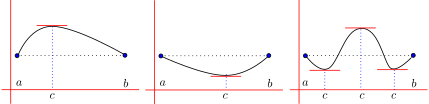
\includegraphics[height=3.5cm]{extra/rolle}
\end{center}
\end{fig}
There can, of course, also be multiple points at which the derivative is zero --- but
there must always be at least one. Notice, however, the theorem\footnote{Notice this is
very similar to the intermediate value theorem (see Theorem~\ref{thm ivt})}
does not tell us the value of $c$, just that such a $c$ must exist.

\begin{eg}\label{eg_2_13_1}
We can use Rolle's theorem to show that the function
\begin{align*}
  f(x) &= \sin(x)-\cos(x)
\end{align*}
has a point $c$ between $0$ and $\frac{3\pi}{2}$ so that $f'(c)=0$.


To apply Rolle's theorem we first have to show the function satisfies the conditions of
the theorem on the interval $[0,\frac{3\pi}{2}]$.
\begin{itemize}
 \item Since $f$ is the sum of sine and cosine it is continuous on the interval and also
differentiable on the interval.
\item Further, since
\begin{align*}
  f(0) &= \sin 0 - \cos 0 = 0-1 = -1  \\
  f\left(\frac{3\pi}{2}\right) &= \sin\frac{3\pi}{2} - \cos\frac{3\pi}{2} = -1-0 = -1
\end{align*}
  we can now apply Rolle's theorem.
\item Rolle's theorem implies that there must be a point $c \in (0,3\pi/2)$ so that
$f'(c) =0$.
\end{itemize}
While Rolle's theorem doesn't tell us the value of $c$, this example is sufficiently
simple that we can find it directly.
\begin{align*}
  f'(x) &= \cos x + \sin x\\
  f'(c) &= \cos c + \sin c  =  0 & \text{rearrange}\\
  \sin c&= - \cos c & \text{and divide by $\cos c$} \\
  \tan c &= -1
\end{align*}
Hence $c = \frac{3\pi}{4}$. We have sketched the function and the relevant points below.
\begin{efig}
\begin{center}
 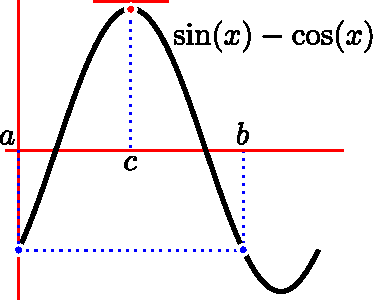
\includegraphics[height=3.5cm]{extra/rolle_sketch}
\end{center}
\end{efig}
\end{eg}
A more substantial application of Rolle's theorem (in conjunction with the intermediate
value theorem --- Theorem~\ref{thm ivt}) is to show that a function does not have
multiple zeros in an interval:
\begin{eg}\label{eg_2_13_2}
Show that the equation $2x-1=\sin(x)$ has exactly 1 solution.
\begin{itemize}
\item Start with a rough sketch of each side of the equation
\begin{efig}
\begin{center}
 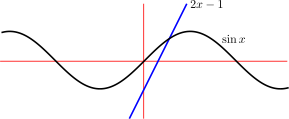
\includegraphics[height=4cm]{extra/rolle_sketch2}
\end{center}
\end{efig}
This seems like it should be true.

\item Notice that the problem we are trying to solve is equivalent to showing
that the function
\begin{align*}
  f(x) &= 2x-1-\sin(x)
\end{align*}
has only a single zero.
\item Since $f(x)$ is the sum of a polynomial and a sine function, it is continuous and
differentiable everywhere. Thus we can apply both the IVT and Rolle's theorem.
\item Notice that $f(0)=-1$ and $f(2) = 4-1-\sin(2) = 3-\sin(2) \geq 2$, since $-1\leq
\sin(2) \leq 1$. Thus by the IVT we know there is at least one number $c$ between $0$ and
$2$ so that $f(c)=0$.

\item But our job is only half done --- this shows that there is at least one zero, but
it does not tell us there is no more than one. We have more work to do, and Rolle's
theorem is the tool we need.

\item Consider what would happen if $f(x)$ is zero in 2 places --- that is, there are
numbers $a,b$ so that $f(a)=f(b)=0$.
\begin{itemize}
 \item Since $f(x)$ is differentiable everywhere and $f(a)=f(b)=0$, we can apply Rolle's
theorem.
\item Hence we know there is a point $c$ between $a$ and $b$ so that $f'(c)=0$.
\item But let us examine $f'(x)$:
\begin{align*}
  f'(x) &= 2- \cos x
\end{align*}
Since $-1\leq \cos x \leq 1$, we must have that $f'(x) \geq 1$.
\item But this contradicts Rolle's theorem which tells us there must be a point at which
the derivative is zero.
\end{itemize}
Thus the function cannot be zero at two different places --- otherwise we'd have a
contradiction.
\end{itemize}
We can actually nail down the value of $c$ using the bisection approach we used in
example~\ref{eg bisection}. If we do this carefully we find that $c \approx
0.887862\dots$

\end{eg}


\subsection*{Back to the MVT}
Rolle's theorem can be generalised in a straight-forward way; given a differentiable
function $f(x)$ we can still say something about $\diff{f}{x}$, even if $f(a) \neq f(b)$.
Consider the following sketch:
\begin{fig}
 \begin{center}
  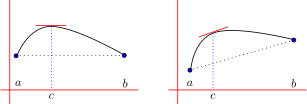
\includegraphics[height=3.5cm]{extra/rolle_to_mvt}
 \end{center}\label{fig rolle_to_mvt}
\end{fig}
All we have done is tilt the picture so that $f(a) < f (b)$. Now we can no longer
guarantee that there will be a point on the graph where the tangent line is horizontal,
but there will be a point where the tangent line is parallel to the secant joining $(a,
f(a))$ to $(b, f(b))$.

To state this in terms of our first scenario back at the beginning of this section,
suppose that you are driving along the $x$--axis. At time $t=a$ you are at $x=f(a)$ and at
time $t=b$ you are at $x=f(b)$. For simplicity, let's suppose that $b>a$ and $f(b)\ge
f(a)$, just like in the above sketch.  Then during the time interval in question you
travelled a net distance of $f(b)-f(a)$. It took you $b-a$ units
of time to travel that distance, so your average velocity was
$\frac{f(b)-f(a)}{b-a}$. You may very well have been going faster than
 $\frac{f(b)-f(a)}{b-a}$ part of the time and slower than
$\frac{f(b)-f(a)}{b-a}$ part of the time. But it is reasonable to guess
that at some time between $t=a$ and $t=b$ your instantaneous velocity was
exactly $\frac{f(b)-f(a)}{b-a}$. The mean value theorem says that, under
reasonable assumptions about $f$, this is indeed the case.
\begin{theorem}[The mean value theorem]
\label{thm:DIFFmvt}
Let $a$ and $b$ be real numbers with $a<b$. And let $f(x)$ be a function so that
\begin{itemize}
 \item $f(x)$ is continuous on the closed interval $a \leq x \leq b$, and
\item $f(x)$ is differentiable on the open interval $a < x < b$
\end{itemize}
then there is a $c \in (a,b)$, such that
\begin{align*}
f'(c)&=\frac{f(b)-f(a)}{b-a}
\intertext{which we can also express as}
  f(b)&=f(a)+f'(c)(b-a).
\end{align*}
\end{theorem}

Let us start to explore the mean value theorem --- which is very frequently known as the
MVT. A simple example to start:
\begin{eg}\label{eg_2_13_3}
Consider the polynomial $f(x)=3x^2-4x+2$ on $[-1,1]$.
\begin{itemize}
 \item Since $f$ is a polynomial it is continuous on the interval and also differentiable
on the interval. Hence we can apply the MVT.
\item The MVT tells us that there is a point $c \in (-1,1)$ so that
\begin{align*}
  f'(c) &= \frac{f(1)-f(-1)}{1-(-1)} = \frac{1-9}{2} =-4
\end{align*}
\end{itemize}
This example is sufficiently simple that we can find the point $c$ and the corresponding
tangent line:
\begin{itemize}
 \item The derivative is
\begin{align*}
  f'(x) &= 6x-4
\end{align*}
\item So we need to solve $f'(c)=-4$:
\begin{align*}
  6c-4 &= -4
\end{align*}
which tells us that $c=0$.
\item The tangent line has slope $-4$ and passes through $(0,f(0))=(0,2)$, and so is
given by
\begin{align*}
  y &= -4x+2
\end{align*}
\item The secant line joining $(-1,f(-1))=(-1,9)$ to $(1,f(1))=(1,1)$ is just
\begin{align*}
  y &= 5-4x
\end{align*}
\item Here is a sketch of the curve and the two lines:
\begin{efig}
\begin{center}
 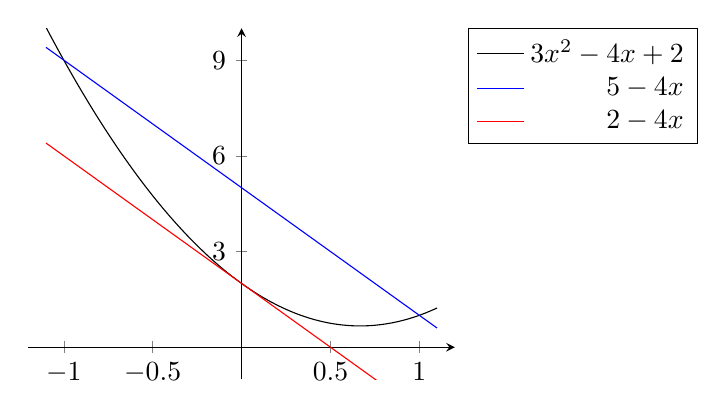
\begin{tikzpicture}
\begin{axis}[
  width=7cm,
  legend style={
    cells={anchor=east},
    legend pos=outer north east,
  },
  axis x line=center, axis y line=center,
  xmax=1.2,xmin=-1.2, xtick={-1,-0.5,0.5,1},
  ymin=-1, ymax=10,
  ytick={0,3,6,9},
  yticklabels={0,3,6,9}
  ]
\addplot[black,domain=-1.1:1.1,samples=100] {3*x*x-4*x+2}; \addlegendentry{$3x^2-4x+2$}
\addplot[blue,domain=-1.1:1.1,samples=100] {5-4*x};  \addlegendentry{$5-4x$}
\addplot[red,domain=-1.1:1.1,samples=100] {2-4*x};  \addlegendentry{$2-4x$}
\end{axis}
\end{tikzpicture}
\end{center}
\end{efig}
\end{itemize}

\end{eg}

\begin{eg}\label{eg:mvtg}
We can return to our initial car-motivated examples. Say you are driving along a straight
road in a car that can go at most $80km/h$. How far can you go in 2 hours? --- the answer
is easy, but we can also solve this using MVT.
\begin{itemize}
 \item Let $s(t)$ be the position of the car in $km$ at time $t$ measured in hours.
\item Then $s(0)=0$ and $s(2)=q$, where $q$ is the quantity that we need to bound.
\item We are told that $| s'(t) | \leq 80$, or equivalently
\begin{align*}
-80 \leq s'(t) \leq 80
\end{align*}
\item By the MVT there is some $c$ between 0 and 2 so that
\begin{align*}
  s'(c) &= \frac{q-0}{2} = \frac{q}{2}
\end{align*}
\item Now since $-80 \leq s'(c) \leq 80$ we must have $-80 \leq q/2 \leq 80$ and hence
$-160 \leq q=s(2) \leq 160$.
\end{itemize}
\end{eg}
More generally if we have some information about the derivative, then we can use the
MVT to leverage this information to tell us something about the function.
\begin{eg}\label{eg_2_13_4}
Let $f(x)$ be a differentiable function so that
\begin{align*}
  f(1)&=10 &\text{ and }&& -1 \leq f'(x) \leq 2 \text{ everywhere}
\end{align*}
Obtain upper and lower bounds on $f(5)$.


Okay --- what do we do?
\begin{itemize}
 \item Since $f(x)$ is differentiable we can use the MVT.
 \item Say $f(5)=q$, then the MVT tells us that there is some $c$ between $1$ and $5$ such
  that
\begin{align*}
 f'(c) &=\frac{q-10}{5-1} = \frac{q-10}{4}
\end{align*}
\item But we know that $-1 \leq f'(c) \leq 2$, so
\begin{align*}
-1 &\leq f'(c) \leq 2 \\
-1 & \leq \frac{q-10}{4} \leq 2 \\
  -4 & \leq q-10 \leq 8 \\
  6 \leq q \leq 18
\end{align*}
\item Thus we must have $6 \leq f(5) \leq 18$.
\end{itemize}
\end{eg}

\subsubsection*{(Optional) --- Why is the MVT True?}
We won't give a real proof for this theorem, but we'll look at a picture
which shows why it is true. Here is the picture. It contains a sketch of
the graph of $f(x)$, with $x$ running from $a$ to $b$, as well as
a line segment which is the secant of the graph from the point
$\big(a\,,f(a)\big)$ to the point $\big(b\,,f(b)\big)$. The slope of
the secant is exactly $\frac{f(b)-f(a)}{b-a}$.
\vadjust{
    \begin{efig}
    \begin{center}
       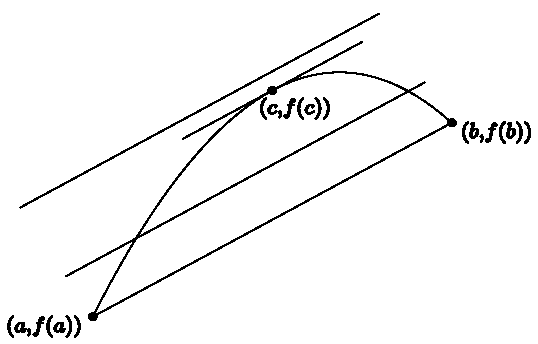
\includegraphics{mvtc}
    \end{center}
    \end{efig}
}
Remember that we are looking for a point, $\big(c\,,f(c)\big)$, on the
graph of $f(x)$ with the property that $f'(c)=\frac{f(b)-f(a)}{b-a}$,
i.e. with the property that the slope of the tangent line at
$\big(c\,,f(c)\big)$ is the same as the slope of the secant.
So imagine that you start moving the secant upward, carefully keeping
the moved line segment parallel to the secant. So the slope of the
moved line segment is always exactly  $\frac{f(b)-f(a)}{b-a}$.
When we first start moving the line segment it is not tangent to the curve ---
it crosses the curve. This is illustrated in the figure by the second line
segment from the bottom.
If we move the line segment too far it does not touch the curve at all.
This is illustrated in the figure by the top segment. But if we stop
moving the line segment just before it stops intersecting the curve at
all, we get exactly the tangent line to the curve at the point on the curve
that is farthest from the secant. This tangent line has exactly the desired
slope. This is illustrated in the figure by the third line
segment from the bottom.

\subsection*{Be Careful with Hypotheses}
\label{warning:mvt}
The mean value theorem has hypotheses --- $f(x)$ has to be continuous
for $a\le x\le b$ and has to be differentiable for $a<x<b$.
If either hypothesis is violated, the conclusion of the mean value theorem
can fail. That is, the curve $y=f(x)$ need not have a
tangent line at some $x=c$ between $a$ and $b$ whose slope, $f'(c)$,
is the same as the slope, $\frac{f(b)-f(a)}{b-a}$, of the secant joining
the points $\big(a\,,f(a)\big)$ and $\big(b\,,f(b)\big)$ on the
curve. If $f'(x)$ fails to exist for even a single value of $x$ between
$a$ and $b$, all bets are off. The following two examples illustrate this.

\begin{eg}\label{eg:mvtd}
For the first ``bad'' example, $a=0$, $b=2$ and
\smallskip
\begin{align*}
f(x) = \begin{cases}
           0  & \text{if }x \le 1 \\
           1 & \text{if }x>1
       \end{cases}
\hskip0.8in  \smash{\raisebox{-0.5\height}{\includegraphics{mvtd}}}
\end{align*}
\smallskip
\noindent
For this example, $f'(x)=0$ at every $x$ where it is defined. That is,
at every $x\ne 1$. But the slope of the secant joining
$\big(a\,,f(a)\big)=(0,0)$ and $\big(b\,,f(b)\big)=(2,1)$
is $\frac{1}{2}$.
\end{eg}


\begin{eg}\label{eg:mvte}
For the second ``bad''  example, $a=-1$, $b=1$ and $f(x)=|x|$.
For this function
\smallskip
\begin{align*}
f'(x) = \begin{cases}
           -1  & \text{if }x < 0 \\
            \text{undefined} & \text{if }x=0\\
           1 & \text{if }x>0
       \end{cases}
\hskip0.8in  \smash{\raisebox{-0.5\height}{\includegraphics{mvte}}}
\end{align*}
\smallskip
\noindent
For this example, $f'(x)=\pm 1$ at every $x$ where it is defined. That is,
at every $x\ne 0$. But the slope of the secant joining
$\big(a\,,f(a)\big)=(-1,1)$ and $\big(b\,,f(b)\big)=(1,1)$
is $0$.
\end{eg}


\begin{eg}\label{eg:mvtf}
Here is one ``good'' example, where the hypotheses of the mean value theorem
are satisfied. Let $f(x)=x^2$. Then $f'(x)=2x$. For any $a<b$,
\begin{align*}
\frac{f(b)-f(a)}{b-a}=\frac{b^2-a^2}{b-a}=b+a
\end{align*}
So $f'(c)=2c$ is exactly $\frac{f(b)-f(a)}{b-a}$ when $c=\frac{a+b}{2}$,
which, in this example, happens to be exactly half way between $x=a$ and
$x=b$.
    \begin{efig}
    \begin{center}
       \includegraphics{mvtf}
    \end{center}
    \end{efig}
\end{eg}

Recall from Section \ref{sec_2_3} that if $f'(c)>0$, then $f(x)$ is 
increasing at $x=c$.
A simple consequence of the mean value theorem is that if you know the
sign of $f'(c)$ for all $c$'s between $a$ and $b$, with $b>a$, then
$f(b)-f(a) = f'(c) (b-a)$ must have the same sign.
\begin{cor}[Consequences of the mean value theorem]
\label{cor:DIFFmvtcons}
Let $A$ and $B$ be real numbers with $A<B$.
Let function $f(x)$ be defined and continuous on
the closed interval $A\le x\le B$ and be differentiable on the
open interval $A<x<B$.
\begin{enumerate}[(a)]
\item If $f'(c)=0$ for all $A<c<B$, then $f(b)=f(a)$ for all
$A\le a<b\le B$.\\
--- That is, $f(x)$ is constant on $A\le x\le B$.
\item If $f'(c)\ge 0$ for all $A<c<B$, then $f(b)\ge f(a)$ for all
$A\le a\le b\le B$.\\
--- That is, $f(x)$ is increasing on $A\le x\le B$.
\item If $f'(c)\le 0$ for all $A<c<B$, then $f(b)\le f(a)$ for all
$A\le a \le b\le B$.\\
--- That is, $f(x)$ is decreasing on $A\le x\le B$.
\end{enumerate}

\end{cor}
It is not hard to see why the above is true:
\begin{itemize}
 \item Say $f'(x)=0$ at every point in the interval $[A,B]$. Now pick any $a,b \in [A,B]$
with $a<b$. Then the MVT tells us that there is $c \in (a,b)$ so that
\begin{align*}
  f'(c) &= \frac{f(b)-f(a)}{b-a}
\end{align*}
If $f(b) \neq f(a)$ then we must have that $f'(c) \neq 0$ --- contradicting what we are
told about $f'(x)$. Thus we must have that $f(b)=f(a)$.

\item Similarly, say $f'(x) \geq 0$ at every point in the interval $[A,B]$. Now pick any
$a,b \in [A,B]$  with $a<b$. Then the MVT tells us that there is $c \in (a,b)$ so that
\begin{align*}
  f'(c) &= \frac{f(b)-f(a)}{b-a}
\end{align*}
Since $b>a$, the denominator is positive. Now if $f(b) < f(a)$ the numerator would be
negative, making the right-hand side negative, and contradicting what we are told about
$f'(x)$. Hence we must have $f(b)\ge f(a)$.
\end{itemize}

A nice corollary of the above corollary is the following:
\begin{cor}\label{cor equal diff}
If $f'(x) = g'(x)$ for all $x$ in the open interval $(a,b)$, then $f-g$ is a constant on
$(a,b)$. That is $f(x)=g(x)+c$, where $c$ is some constant.
\end{cor}
We can prove this by setting $h(x)=f(x)-g(x)$. Then $h'(x)=0$ and so the previous
corollary tells us that $h(x)$ is constant.

\begin{eg}\label{eg_2_13_5}
Using this corollary we can prove results like the following:
\begin{align*}
  \arcsin x + \arccos x &= \frac{\pi}{2} & \mbox{for all } -1 < x < 1
\end{align*}
How does this work? Let $f(x) = \arcsin x + \arccos x$. Then
\begin{align*}
  f'(x) &= \frac{1}{\sqrt{1-x^2}} + \frac{-1}{\sqrt{1-x^2}} = 0
\end{align*}
Thus $f$ must be a constant. To find out which constant, we can just check its value at a
convenient point, like $x=0$.
\begin{align*}
  \arcsin(0) + \arccos(0) &= \pi/2 + 0 = \pi/2
\end{align*}
Since the function is constant, this must be the value.
\end{eg}


%%%%%%%%%%%%%%%%%%%%%%%%%%%%%%%%%%%%%%%%%%%%%%
\section{Higher Order Derivatives}\label{sec higher diff}
%%%%%%%%%%%%%%%%%%%%%%%%%%%%%%%%%%%%%%%%%%%%%%

The operation of differentiation takes as input one function,
$f(x)$, and produces as output another function, $f'(x)$. Now $f'(x)$ is
once again a function. So we can differentiate it again, assuming that
it is differentiable, to create a third function, called the second
derivative of $f$. And we can differentiate the second derivative again
to create a fourth function, called the third derivative of $f$.
And so on.
\begin{notn}\label{not:higherOrdDeriv}
\begin{itemize}
\item $f''(x)$ and $f^{(2)}(x)$  and $\ddiff{2}{f}{x}(x)$ all mean
$\diff{}{x}\big(\diff{}{x}f(x)\big)$
\item $f'''(x)$ and $f^{(3)}(x)$  and $\ddiff{3}{f}{x}(x)$ all mean
$\diff{}{x}\big(\diff{}{x}\big(\diff{}{x}f(x)\big)\big)$
\item $f^{(4)}(x)$  and $\ddiff{4}{f}{x}(x)$ both mean
$\diff{}{x}\big(\diff{}{x}\big(\diff{}{x}\big(\diff{}{x}f(x)\big)\big)\big)$
\item and so on.
\end{itemize}
\end{notn}

Here is a simple example. Then we'll think a little about the significance
of second order derivatives. Then we'll do a more a computationally complex
example.

\begin{eg}\label{eg:higherOrdDerivA}
Let $n$ be a natural number and let $f(x)= x^n$. Then
\begin{align*}
\diff{}{x}x^n&=nx^{n-1} \\
\ddiff{2}{}{x}x^n&=\diff{}{x}\big(nx^{n-1}\big)=n(n-1)x^{n-2} \\
\ddiff{3}{}{x}x^n&=\diff{}{x}\big(n(n-1)x^{n-2}\big)=n(n-1)(n-2)x^{n-3}
\end{align*}
Each time we differentiate, we bring down the exponent, which is exactly
one smaller than the previous exponent brought down, and we reduce the
exponent by one. By the time we have differentiated $n-1$ times,
the exponent has decreased to $n-(n-1)=1$ and we have brought down the
factors $n(n-1)(n-2)\cdots 2$. So
\begin{align*}
\ddiff{{n-1}}{}{x}x^n&=n(n-1)(n-2)\cdots 2x
\end{align*}
and
\begin{align*}
\ddiff{n}{}{x}x^n&=n(n-1)(n-2)\cdots 1
\end{align*}
The product of the first $n$ natural numbers, $1\cdot 2\cdot 3\cdot \cdots
\cdot n,$ is called ``$n$ factorial'' and is denoted $n!$. So we can also
write
\begin{align*}
\ddiff{n}{}{x}x^n&=n!
\end{align*}
If $m>n$, then
\begin{align*}
\ddiff{m}{}{x}x^n&=0
\end{align*}
\end{eg}

\begin{eg}\label{eg_2_14_1}
Recall that the derivative $v'(a)$ is the (instantaneous) rate of
change of the function $v(t)$ at $t=a$. Suppose that you are walking on
the $x$--axis and that $x(t)$ is your $x$--coordinate at time $t$.
Also suppose, for simplicity, that you are moving from left to right.
Then $v(t)=x'(t)$ is your velocity at time $t$ and $v'(a)=x''(a)$ is the
rate at which your velocity is changing at time $t=a$. It is called your
acceleration. In particular, if $x''(a)>0$, then your velocity is increasing,
i.e. you are speeding up, at time $a$. If $x''(a)<0$, then your velocity
is decreasing, i.e. you are slowing down, at time $a$. That's one
interpretation of the second derivative.
\end{eg}

\begin{eg}[Example \ref{eg:DIFFimpldiffD}, continued]\label{eg:higherOrdDerivC}
Find $y''$ if $y=y^3+xy+x^3$.

\soln This problem concerns some function $y(x)$ that is not
given to us explicitly. All that we are told is that $y(x)$ satisfies
\begin{equation}
y(x)=y(x)^3+xy(x)+x^3
\tag{E1}
\end{equation}
for all $x$. We are asked to find $y''(x)$. We cannot solve this
equation to get an explicit formula for $y(x)$.  So we use implicit
differentiation, as we did in Example \ref{eg:DIFFimpldiffD}. That is, we apply
$\diff{}{x}$ to both sides of (E1). This gives
\begin{equation}
y'(x)=3y(x)^2\,y'(x)+y(x)+x\,y'(x)+3x^2
%\implies \big[1-x-3y(x)^2\big]y'(x) = y(x)+3x^2
\tag{E2}
\end{equation}
which we can solve for $y'(x)$, by moving all $y'(x)$'s to the left hand
side, giving
\begin{equation*}
 \big[1-x-3y(x)^2\big]y'(x) = y(x)+3x^2
\end{equation*}
and then dividing across.
\begin{equation}
y'(x) = \frac{y(x)+3x^2}{1-x-3y(x)^2}
\tag{E3}\end{equation}
To get $y''(x)$, we have two options.

\noindent\emph{Method 1.}\ \ \  Apply $\diff{}{x}$ to both sides of (E2).
This gives
\begin{equation*}
y''(x)=3y(x)^2\,y''(x)+6y(x)\,y'(x)^2+2y'(x)+x\,y''(x)+6x
\end{equation*}
We can now solve for $y''(x)$, giving
\begin{equation}
y''(x) = \frac{6x+2y'(x)+6y(x)y'(x)^2}{1-x-3y(x)^2}
\tag{E4}
\end{equation}
Then we can substitute in (E3), giving
\begin{align*}
y''(x) &= 2\frac{3x+ \frac{y(x)+3x^2}{1-x-3y(x)^2}
              +3y(x) \big(\frac{y(x)+3x^2}{1-x-3y(x)^2}\big)^2}
         {1-x-3y(x)^2} \\
&= 2\frac{3x{[1-x-3y(x)^2]}^2+ [y(x)+3x^2][1-x-3y(x)^2]
              +3y(x) {[y(x)+3x^2]}^2}{{[1-x-3y(x)^2]}^3}
\end{align*}

\noindent\emph{Method 2.}\ \ \  Alternatively, we can also differentiate (E3).
\begin{align*}
y''(x) &= \frac{[y'(x)+6x][1-x-3y(x)^2]-
           [y(x)+3x^2][-1-6y(x)y'(x)]}{{[1-x-3y(x)^2]}^2} \\[0.05in]
&= \frac{[\frac{y(x)+3x^2}{1-x-3y(x)^2}+6x][1-x-3y(x)^2]-
           [y(x)+3x^2][-1-6y(x)\frac{y(x)+3x^2}{1-x-3y(x)^2}]}
                                       {{[1-x-3y(x)^2]}^2}\\[0.05in]
&= \frac{2[y(x)+3x^2][1-x-3y(x)^2]+6x{[1-x-3y(x)^2]}^2
           +6y(x){[y(x)+3x^2]}^2}
                                       {{[1-x-3y(x)^2]}^3}
\end{align*}

\noindent\emph{Remark 1.}\ \ \ We have now computed $y''(x)$ --- sort of.
The answer is in terms of $y(x)$, which we don't know. Since we cannot
get an explicit formula for $y(x)$, there's not a great deal that we can do,
in general.

\noindent\emph{Remark 2.}\ \ \ Even though we cannot solve
$y=y^3+xy+x^3$ explicitly for $y(x)$, for general $x$, it is sometimes
possible to solve equations like this for some special values of $x$.
In fact, we saw in Example \ref{eg:DIFFimpldiffD} that when $x=1$,
the given equation reduces to $y(1)=y(1)^3+1\cdot y(1)+1^3$, or $y(1)^3=-1$,
which we can solve to get $y(1)=-1$. Substituting into (E2),
as we did in  Example \ref{eg:DIFFimpldiffD} gives
\begin{equation*}
y'(1) = \frac{-1+3}{1-1-3(-1)^2} = -\frac{2}{3}
\end{equation*}
and substituting into (E4) gives
\begin{equation*}
y''(1) = \frac{6+2\big(-\frac{2}{3}\big)+6(-1)\big(-\frac{2}{3}\big)^2}
                             {1-1-3(-1)^2}
   =\frac{6-\frac{4}{3}-\frac{8}{3}}{-3}
   = -\frac{2}{3}
\end{equation*}
(It's a fluke that, in this example, $y'(1)$ and $y''(1)$ happen to be equal.)
So we now know that, even though we can't solve $y=y^3+xy+x^3$ explicitly for
$y(x)$, the graph of the solution passes through $(1,-1)$ and has slope
$-\frac{2}{3}$ (i.e. is sloping downwards by between $30^\circ$ and $45^\circ$)
there and, furthermore, the slope of the graph decreases as $x$
increases through $x=1$.

\begin{efig}
 \begin{center}
 \includegraphics{concaveDown}
 \end{center}
\end{efig}
Here is a sketch of the part of the graph very near $(1, -1)$. The tangent line to the
graph at $(1, -1)$ is also shown. Note that the tangent line is sloping down to the right,
as we expect, and that the graph lies below the tangent line near $(1,-1)$. That's because
the slope $f'(x)$ is decreasing (becoming more negative) as $x$ passes through $1$.


\end{eg}

\begin{warning}\label{warning:dropx}
Many people will suppress the $(x)$ in $y(x)$ when doing
computations like those in Example \ref{eg:higherOrdDerivC}.
This gives shorter, easier to read formulae, like
$y'=\frac{y+3x^2}{1-x-3y^2}$. If you do this, you must never forget
that $y$ is a function of $x$ and is \emph{not} a constant. If you do forget,
you'll make the very serious error of saying that $\diff{y}{x}=0$,
which is false.

\end{warning}


\section{(Optional) --- Is $\lim\limits_{x\to c}f'(x)$ Equal to $f'(c)$?}\label{sec:cont_deriv}

Consider the function
\begin{equation*}
f(x) = \begin{cases}
            \frac{\sin x^2}{x} &\text{if $x\ne 0$} \\
             0                  &\text{if $x=0$}
        \end{cases}
\end{equation*}
For any $x\ne 0$ we can easily use our differentiation rules to find
\begin{align*}
f'(x) = \frac{2x^2\cos x^2 -\sin x^2}{x^2}
\end{align*}
But for $x=0$ none of our usual differentation rules apply. So how do we find $f'(0)$? One obviously legitimate strategy is to directly apply the 
Definition \ref{def:DIFFderiv}
of the derivative. As an alternative, we will now consider the question ``Can one find $f'(0)$ by taking the limit of $f'(x)$ as $x$ tends to zero?''.
There is bad news and there is good news.
\begin{itemize}
\item
The bad news is that,
even for functions $f(x)$ that are differentiable for all $x$, $f'(x)$ need not be continuous. That is, it is \emph{not} always true that 
$\lim_{x\rightarrow 0}f'(x) = f'(0)$. We will see a function for which 
$\lim_{x\rightarrow 0}f'(x) \ne f'(0)$ in 
Example \ref{eg:discontinuous derivative}, below.
\item
The good news is that Theorem \ref{thm:continuous derivative}, below 
provides conditions which are sufficient to guarantee that $f(x)$ is differentiable at $x=0$ and that $\lim_{x\rightarrow 0}f'(x) = f'(0)$.  
\end{itemize}



\begin{eg}\label{eg:discontinuous derivative}
Consider the function
\begin{equation*}
f(x) = \begin{cases}
            x^2\sin\frac{1}{x} &\text{if $x\ne 0$} \\
             0                  &\text{if $x=0$}
        \end{cases}
\end{equation*}
For $x\ne 0$ we have, by the product and chain rules,
\begin{align*}
f'(x)  &= 2x\, \sin\frac{1}{x} + x^2 \left(\cos\frac{1}{x}\right)
                     \left(-\frac{1}{x^2}\right) \\
       &=  2x\, \sin\frac{1}{x} - \cos\frac{1}{x}
\end{align*}
As $\left|\sin\frac{1}{x}\right|\le 1$, we have
\begin{equation*}
\lim_{x\rightarrow 0}2x\, \sin\frac{1}{x}=0
\end{equation*}
On the other hand, as $x$ tends to zero, $\frac{1}{x}$ goes to $\pm\infty$.
So
\begin{equation*}
\lim_{x\rightarrow 0}\cos\frac{1}{x} = DNE
\implies 
\lim_{x\rightarrow 0}f'(x) = DNE
\end{equation*}
We will now see that, despite this, $f'(0)$ is perfectly well defined.
By definition
\begin{align*}
f'(0) &= \lim_{h\to 0}\frac{f(h)-f(0)}{h}  \\
      & = \lim_{h\to 0}\frac{h^2\sin\frac{1}{h}-0}{h} \\
      & = \lim_{h\to 0} h\sin\frac{1}{h} \\
      & = 0\qquad\text{since $\left|\sin\frac{1}{h}\right|\le 1$}
\end{align*}
So $f'(0)$ exists, but is not equal to $\lim_{x\rightarrow 0}f'(x)$,
which does not exist.
\end{eg}
Now for the good news.
%%%%%%%%%%%%%%%
\begin{theorem}\label{thm:continuous derivative}
Let $a<c<b$. Assume that 
\begin{itemize}
\item 
the function $f(x)$ is continous on the interval $a<x<b$ and
\item
is differentiable at every $x$ in the intervals $a<x<c$ and $c<x<b$ and
\item
the limit  $\lim_{x\rightarrow c}f'(x)$ exists.
\end{itemize}
Then $f$ is differentiable at $x=c$ and
\begin{equation*}
f'(c) = \lim_{x\rightarrow c}f'(x)
\end{equation*}
\end{theorem}

\begin{proof}
By hypothesis, there is a number $L$ such that
\begin{equation*}
\lim_{x\rightarrow c}f'(x) = L
\end{equation*}
By definition
\begin{equation*}
f'(c) = \lim_{h\to 0}\frac{f(c+h)-f(c)}{h}
\end{equation*}
By the Mean Value Theorem (Theorem \ref{thm:DIFFmvt}) 
there is, for each $h$,
an (unknown) number $x_h$ between $c$ and $c+h$ such that 
$f'(x_h)=\frac{f(c+h)-f(c)}{h}$. So
\begin{equation*}
f'(c) = \lim_{h\to 0} f'(x_h)
\end{equation*}
As $h$ tends to zero, $c+h$ tends to $c$, and so  $x_h$ is forced to tend 
to $c$, and $f'(x_h)$ is forced to tend to $L$ so that
\begin{equation*}
f'(c) = \lim_{h\to 0} f'(x_h) = L
\end{equation*}
\end{proof}


In the next example we evaluate $f'(0)$ by applying 
Theorem \ref{thm:continuous derivative}.
\begin{eg}\label{eg:continuous derivative}
Let 
\begin{equation*}
f(x) = \begin{cases}
            \frac{\sin x^2}{x} &\text{if $x\ne 0$} \\
             0                  &\text{if $x=0$}
        \end{cases}
\end{equation*}
We have already observed above that, for $x\ne 0$,
\begin{align*}
f'(x) = \frac{2x^2\cos x^2 -\sin x^2}{x^2}
      = 2\cos x^2 - \frac{\sin x^2}{x^2}
\end{align*}
We use Theorem~\ref{thm:continuous derivative} with $c=0$ to show that $f(x)$ is differentiable at $x=0$ and to evaluate $f'(0)$. That theorem 
has two hypotheses that we have not yet verified, namely the continuity of 
$f(x)$ at $x=0$, and the existence of the limit $\lim_{x\rightarrow 0}f'(x)$.
We verify them now.
\begin{itemize}
\item We already know, by Lemma \ref{lem sinhoverh},
that $\lim_{h\rightarrow 0}\frac{\sin h}{h}=1$. So
\begin{align*}
\lim_{x\rightarrow 0}\frac{\sin x^2}{x^2} 
&=\lim_{h\rightarrow 0^+}\frac{\sin h}{h}\qquad\text{with $h=x^2$} \\
&=1
\end{align*}
and
\begin{align*}
\lim_{x\rightarrow 0} f(x) 
&=\lim_{x\rightarrow 0}\frac{\sin x^2}{x}
=\lim_{x\rightarrow 0}x\,\frac{\sin x^2}{x^2}
=\lim_{x\rightarrow 0}x\ \lim_{x\rightarrow 0}\frac{\sin x^2}{x^2}
=0\times 1
=0
\end{align*}
and $f(x)$ is continuous at $x=0$.
\item The limit of the derivative is
\begin{align*}
\lim_{x\rightarrow 0}f'(x) 
&= \lim_{x\rightarrow 0}\left[2\cos x^2 - \frac{\sin x^2}{x^2}\right]
=2\times 1 -1 = 1
\end{align*}
\end{itemize}
So, by Theorem~\ref{thm:continuous derivative}, $f(x)$ is differentiable 
at $x=0$ and $f'(0)=1$.
\end{eg}





\begin{comment}


%%%%%%%%%%%%%%%%%%%%%%%%%%%%%%%%%%%%%%%%%%%%%%
\section{Higher Order Derivatives}
%%%%%%%%%%%%%%%%%%%%%%%%%%%%%%%%%%%%%%%%%%%%%%

The operation of differentiation takes as input one function,
$f(x)$, and produces as output another function, $f'(x)$. Now $f'(x)$ is
once again a function. So we can differentiate it again, assuming that
it is differentiable, to create a third function, called the second
derivative of $f$. And we can differentiate the second derivative again
to create a fourth function, called the third derivative of $f$.
And so on.
\begin{notn}\label{not:higherOrdDeriv}
\begin{itemize}
\item $f''(x)$ and $f^{(2)}(x)$  and $\ddiff{2}{f}{x}(x)$ all mean
$\diff{}{x}\big(\diff{}{x}f(x)\big)$
\item $f'''(x)$ and $f^{(3)}(x)$  and $\ddiff{3}{f}{x}(x)$ all mean
$\diff{}{x}\big(\diff{}{x}\big(\diff{}{x}f(x)\big)\big)$
\item $f^{(4)}(x)$  and $\ddiff{4}{f}{x}(x)$ both mean
$\diff{}{x}\big(\diff{}{x}\big(\diff{}{x}\big(\diff{}{x}f(x)\big)\big)\big)$
\item and so on.
\end{itemize}
\end{notn}

Here is a simple example. Then we'll think a little about the significance
of second order derivatives. Then we'll do a more a computationally complex example.

\begin{eg}\label{eg:higherOrdDerivA}
Let $n$ be a natural number and let $f(x)= x^n$. Then
\begin{align*}
\diff{}{x}x^n&=nx^{n-1} \\
\ddiff{2}{}{x}x^n&=\diff{}{x}\big(nx^{n-1}\big)=n(n-1)x^{n-2} \\
\ddiff{3}{}{x}x^n&=\diff{}{x}\big(n(n-1)x^{n-2}\big)=n(n-1)(n-2)x^{n-3}
\end{align*}
Each time we differentiate, we bring down the exponent, which is exactly
one smaller than the previous exponent brought down, and we reduce the
exponent by one. By the time we have differentiated $n-1$ times,
the exponent has decreased to $n-(n-1)=1$ and we have brought down the
factors $n(n-1)(n-2)\cdots 2$. So
\begin{align*}
\ddiff{{n-1}}{}{x}x^n&=n(n-1)(n-2)\cdots 2x
\end{align*}
and
\begin{align*}
\ddiff{n}{}{x}x^n&=n(n-1)(n-2)\cdots 1
\end{align*}
The product of the first $n$ natural numbers, $1\cdot 2\cdot 3\cdot \cdots
\cdot n,$ is called ``$n$ factorial'' and is denoted $n!$. So we can also
write
\begin{align*}
\ddiff{n}{}{x}x^n&=n!
\end{align*}
If $m>n$, then
\begin{align*}
\ddiff{m}{}{x}x^n&=0
\end{align*}
\end{eg}

Recall that the derivative $v'(a)$ is the (instantaneous) rate of
change of the function $v(t)$ at $t=a$. Suppose that you are walking on
the $x$--axis and that $x(t)$ is your $x$--coordinate at time $t$.
Also suppose, for simplicity, that you are moving from left to right.
Then $v(t)=x'(t)$ is your speed at time $t$ and $v'(a)=x''(a)$ is the
rate at which your speed is changing at time $t=a$. It is called your
acceleration. In particular, if $x''(a)>0$, then your speed is increasing,
i.e. you are speeding up, at time $a$. If $x''(a)<0$, then your speed
is decreasing, i.e. you are slowing down, at time $a$. That's one
interpretation of the second derivative.

Here is another interpretation. Consider the graph $y=f(x)$. Then we know
that $f'(x)$ is the slope of the (tangent line to the) graph at the point
$\big(x\,,\,f(x)\big)$. So $f''(a)$ is the rate at which the slope
at $\big(x\,,\,f(x)\big)$ is changing as $x$ increases through $a$.
If $f''(a)>0$ then the slope is increasing as you move from left to right
through $x=a$. In this case the curve is said to be concave up at $x=a$.
If $f''(a)<0$ then the slope is decreasing as you move from left to right
through $x=a$. In this case the curve is said to be concave down at $x=a$.
Here is a simple example, with a sketch, illustrating this.

\begin{eg}\label{eg:higherOrdDerivB}
Consider the graph $y=f(x)=x^3-3x$. The first two derivatives of the function
$f(x)$ are
\begin{equation*}
f'(x) = 3x^2-3=3(x^2-1)\qquad
f''(x) = 6x
\end{equation*}
So $f'(x)$ is strictly positive when $x^2>1$ (i.e. $x<-1$ or $x>1$),
zero when $x^2=1$ (i.e. $x=\pm 1$) and strictly negative when $x^2<1$
(i.e. $-1<x<1$). And $f''(x)$ is strictly positive when $x>0$,
zero when $x=0$ and strictly negative when $x<0$.
\begin{itemize}
\item When $x<-1$ the graph has positive slope but that slope decreases
(i.e. the tangent line becomes less steep) as $x$ increases. The graph
is concave down.
\item When $-1<x<0$ the graph has negative slope and that slope decreases
(i.e. becomes more negative -- the tangent line becomes steeper) as
$x$ increases. The graph is still concave down.
\item When $0<x<1$ the graph has negative slope but that slope increases
(i.e. becomes less negative -- the tangent line becomes less steep) as
$x$ increases. The graph is concave up.
\item When $x>1$ the graph has positive slope and that slope increases
as $x$ increases. The graph is concave up.
\end{itemize}
Here is a figure containing the graph and some tangent lines near $x=-1$
and near $x=+1$. We see the slope of the tangent lines
decreasing from a positive number through zero to a negative number as
$x$ increases through $-1$. And we see the slope of the tangent lines
increasing from a negative number through zero to a positive number as
$x$ increases through $+1$.

\begin{efig}
 \begin{center}
 \includegraphics{concaveUpDown}
 \end{center}
\end{efig}

\end{eg}


Now here is a more computationally complex example.

\begin{eg}[Example \ref{eg:DIFFimpldiffD}, continued]\label{eg:higherOrdDerivC}
Find $y''$ if $y=y^3+xy+x^3$.

\soln This problem concerns some function $y(x)$ that is not
given to us explicitly. All that we are told is that $y(x)$ satisfies
\begin{equation}\label{eq:hoDerivBa}
y(x)=y(x)^3+xy(x)+x^3
\end{equation}
for all $x$. We are asked to find $y''(x)$. We cannot solve this
equation to get an explicit formula for $y(x)$.  So we use implicit
differentiation, as we did in Example \ref{eg:DIFFimpldiffD}. That is, we apply
$\diff{}{x}$ to both sides of \eqref{eq:hoDerivBa}. This gives
\begin{equation}\label{eq:hoDerivBb}
y'(x)=3y(x)^2\,y'(x)+y(x)+x\,y'(x)+3x^2
%\implies \big[1-x-3y(x)^2\big]y'(x) = y(x)+3x^2
\end{equation}
which we can solve for $y'(x)$, by moving all $y'(x)$'s to the left hand
side, giving
\begin{equation*}
 \big[1-x-3y(x)^2\big]y'(x) = y(x)+3x^2
\end{equation*}
and then dividing across.
\begin{equation}\label{eq:hoDerivBc}
y'(x) = \frac{y(x)+3x^2}{1-x-3y(x)^2}
\end{equation}
To get $y''(x)$, we have two options.

\noindent\emph{Method 1.}\ \ \  Apply $\diff{}{x}$ to both sides of \eqref{eq:hoDerivBb}.
This gives
\begin{equation*}
y''(x)=3y(x)^2\,y''(x)+6y(x)\,y'(x)^2+2y'(x)+x\,y''(x)+6x
\end{equation*}
We can now solve for $y''(x)$, giving
\begin{equation}\label{eq:hoDerivBd}
y''(x) = \frac{6x+2y'(x)+6y(x)y'(x)^2}{1-x-3y(x)^2}
\end{equation}
Then we can substitute in \eqref{eq:hoDerivBc}, giving
\begin{align*}
y''(x) &= 2\frac{3x+ \frac{y(x)+3x^2}{1-x-3y(x)^2}
              +3y(x) \big(\frac{y(x)+3x^2}{1-x-3y(x)^2}\big)^2}
         {1-x-3y(x)^2} \\
&= 2\frac{3x{[1-x-3y(x)^2]}^2+ [y(x)+3x^2][1-x-3y(x)^2]
              +3y(x) {[y(x)+3x^2]}^2}{{[1-x-3y(x)^2]}^3}
\end{align*}

\noindent\emph{Method 2.}\ \ \  Alternatively, we can also differentiate
\eqref{eq:hoDerivBc}.
\begin{align*}
y''(x) &= \frac{[y'(x)+6x][1-x-3y(x)^2]-
           [y(x)+3x^2][-1-6y(x)y'(x)]}{{[1-x-3y(x)^2]}^2} \\[0.05in]
&= \frac{[\frac{y(x)+3x^2}{1-x-3y(x)^2}+6x][1-x-3y(x)^2]-
           [y(x)+3x^2][-1-6y(x)\frac{y(x)+3x^2}{1-x-3y(x)^2}]}
                                       {{[1-x-3y(x)^2]}^2}\\[0.05in]
&= \frac{2[y(x)+3x^2][1-x-3y(x)^2]+6x{[1-x-3y(x)^2]}^2
           +6y(x){[y(x)+3x^2]}^2}
                                       {{[1-x-3y(x)^2]}^3}
\end{align*}

\noindent\emph{Remark 1.}\ \ \ We have now computed $y''(x)$ --- sort of.
The answer is in terms of $y(x)$, which we don't know. Since we cannot
get an explicit formula for $y(x)$, there's not a great deal that we can do,
in general.

\noindent\emph{Remark 2.}\ \ \ Even though we cannot solve
$y=y^3+xy+x^3$ explicitly for $y(x)$, for general $x$, it is sometimes
possible to solve equations like this for some special values of $x$.
In fact, we saw in Example \ref{eg:DIFFimpldiffD} that when $x=1$,
the given equation reduces to $y(1)=y(1)^3+1\cdot y(1)+1^3$, or $y(1)^3=-1$,
which we can solve to get $y(1)=-1$. Substituting into \eqref{eq:hoDerivBb},
as we did in  Example \ref{eg:DIFFimpldiffD} gives
\begin{equation*}
y'(1) = \frac{-1+3}{1-1-3(-1)^2} = -\frac{2}{3}
\end{equation*}
and substituting into \eqref{eq:hoDerivBd} gives
\begin{equation*}
y''(1) = \frac{6+2\big(-\frac{2}{3}\big)+6(-1)\big(-\frac{2}{3}\big)^2}
                             {1-1-3(-1)^2}
   =\frac{6-\frac{4}{3}-\frac{8}{3}}{-3}
   = -\frac{2}{3}
\end{equation*}
(It's a fluke that, in this example, $y'(1)$ and $y''(1)$ happen to be equal.)
So we now know that, even though we can't solve $y=y^3+xy+x^3$ explicitly for
$y(x)$, the graph of the solution passes through $(1,-1)$ and has slope
$-\frac{2}{3}$ (i.e. is sloping downwards by between $30^\circ$ and $45^\circ$)
there and, furthermore, the slope of the graph decreases as $x$
increases through $x=1$.  The graph is concave down near $x=1$. Here
is a sketch of the part of the graph very near $(1,-1)$. The tangent
line to the graph at $(1,-1)$ is also shown. Note that the tangent line
is sloping down to the right, as we expect, and that the graph lies below
the tangent line near $(1,-1)$. That is typical of concave down graphs.

\begin{efig}
 \begin{center}
 \includegraphics{concaveDown}
 \end{center}
\end{efig}


\end{eg}

\begin{warning}\label{warning:dropx}
Many people will suppress the $(x)$ in $y(x)$ when doing
computations like those in Example \ref{eg:higherOrdDerivC}.
This gives shorter, easier to read formulae, like
$y'=\frac{y+3x^2}{1-x-3y^2}$. If you do this, you must never forget
that $y$ is a function of $x$ and is \emph{not} a constant. If you do forget,
you'll make the very serious error of saying that $\diff{y}{x}=0$,
which is false.

\end{warning}


\intremark{ %%%% INTERNAL REMARK - another, less good, example
\begin{eg}\label{eg:higherOrdDerivNU}
Find $y''$ if $4y+x^4+y^4=6$.

\soln This problem concerns some function $y(x)$ that is not
given to us explicitly. All that we are told is that $y(x)$ satisfies
\begin{equation}\label{eq:hoDerivBa}
4y(x) +x^4+y(x)^4=6
\end{equation}
for all $x$. We are asked to find $y''(x)$. We cannot solve this
equation to get an explicit formula for $y(x)$.  So we use implicit
differentiation, as we did in Example \ref{eg:DIFFimpldiffD}. That is, we apply
$\diff{}{x}$ to both sides of \eqref{eq:hoDerivBa}. This gives
\begin{equation}\label{eq:hoDerivBb}
4y'(x) +4x^3+4y(x)^3y'(x)=0
\implies y'(x) +x^3+y(x)^3y'(x)=0
\end{equation}
which we can solve for $y'(x)$.
\begin{equation}\label{eq:hoDerivBc}
y'(x) = -\frac{x^3}{1+y(x)^3}
\end{equation}
To get $y''(x)$, we have two options.

\noindent\emph{Method 1.}\ \ \  Apply $\diff{}{x}$ to both sides of \eqref{eq:hoDerivBb}.
This gives
\begin{equation}\label{eq:hoDerivBd}
y''(x) +3x^2+3y(x)^2y'(x)^2+y(x)^3y''(x)=0
\end{equation}
We can now solve for $y''(x)$, giving
\begin{equation*}
y''(x) = -\frac{3x^2+3y(x)^2y'(x)^2}{1+y(x)^3}
\end{equation*}
and then substitute in \eqref{eq:hoDerivBc}, giving
\begin{equation*}
y''(x) = -3\frac{x^2+y(x)^2\frac{x^6}{{[1+y(x)^3]}^2}}{1+y(x)^3}
= -3\frac{x^2{[1+y(x)^3]}^2+y(x)^2x^6}{{[1+y(x)^3]}^3}
\end{equation*}

\noindent\emph{Method 2.}\ \ \  Alternatively, we can also differentiate
\eqref{eq:hoDerivBc}.
\begin{align*}
y''(x) &= -\frac{3x^2[1+y(x)^3]-x^3\,3y(x)^2y'(x)}{{[1+y(x)^3]}^2}
= -\frac{3x^2[1+y(x)^3]+x^3\,3y(x)^2\frac{x^3}{1+y(x)^3}}{{[1+y(x)^3]}^2}\\
&= -3\frac{x^2{[1+y(x)^3]}^2+y(x)^2x^6}{{[1+y(x)^3]}^3}
\end{align*}

\noindent\emph{Remark 1.}\ \ \ We have now computed $y''(x)$ --- sort of.
The answer is in terms of $y(x)$, which we don't know. Since we cannot
get an explicit formula for $y(x)$, there's not a great deal that we can do.

%\noindent\emph{Remark 2.}\ \ \ Even though we cannot solve
%$4y(x) +x^4+y(x)^4=6$ explicitly for $y(x)$, for general $x$, it is sometimes
%possible to solve equations like this for some special values of $x$.
%For example, when $x=1$, the equation reduces to
%\begin{equation*}
%4y(1) + y(1)^4=5
%\end{equation*}
\end{eg}
}  %%% END INTERNAL REMARK - another, less good, example


%%%%%%%%%%%%%%%%%%%%%%%%%%%%%%%%%%%%%%%%%%%%%%
\section{Approximating Functions Near a Specified Point --- Taylor
Polynomials}\label{sec:DIFFTaylor}
%%%%%%%%%%%%%%%%%%%%%%%%%%%%%%%%%%%%%%%%%%%%%5
Suppose that you are interested in the values of some function $f(x)$ for
$x$ near some fixed point $a$. The function is too complicated to work
with directly. So you wish to work instead with some other function $F(x)$
that is both simple and a good approximation to $f(x)$ for $x$ near
$a$. We'll consider a couple of examples of this scenario later.
First, we develop several different approximations.

%%%%%%%%%%%%%%%%%%%%%%%%%%%%%%%%%%%%%%%%%%%%%%%%%%%%%%%%%%%%%%%%%%%%%%
\subsection{Zeroth Approximation --- the Constant Approximation}
%%%%%%%%%%%%%%%%%%%%%%%%%%%%%%%%%%%%%%%%%%%%%%%%%%%%%%%%%%%%%%%%%%%%%%
The simplest functions are those that are constants. The first
approximation will be by a constant function. That is, the approximating
function will have the form $F(x)=A$, for some constant $A$. To ensure
that $F(x)$ is a good approximation for $x$ close to $a$, we choose
$A$ so that $f(x)$ and $F(x)$ take exactly the same value when $x=a$.
\begin{equation*}
F(x)=A\qquad\text{so}\qquad F(a)=A=f(a)\implies A=f(a)
\end{equation*}
Our first, and crudest, approximation rule is
\begin{equation}\label{eq:constApprox}
f(x)\approx f(a)
\end{equation}
Here is a figure showing the graphs of a typical $f(x)$ and approximating
function $F(x)$.
\vadjust{
    \begin{efig}
    \begin{center}
       \includegraphics{approx1}
    \end{center}
    \end{efig}
}
At $x=a$, $f(x)$ and $F(x)$ take the same value. For $x$ very near $a$,
the values of $f(x)$ and $F(x)$ remain close together. But the quality
of the approximation deteriorates fairly quickly as $x$ moves
away from $a$.

%%%%%%%%%%%%%%%%%%%%%%%%%%%%%%%%%%%%%%%%%%%%%%%%%%%%%%%%%%%%%%%%%%%%%%
\subsection{First Approximation --- the Tangent Line, or Linear, Approximation}
%%%%%%%%%%%%%%%%%%%%%%%%%%%%%%%%%%%%%%%%%%%%%%%%%%%%%%%%%%%%%%%%%%%%%%
We now develop a better approximation by allowing the approximating function
to be a linear function of $x$ and not just a constant function. That is,
we allow $F(x)$ to be of the form $A+Bx$, for some constants $A$ and $B$.
To ensure that $F(x)$ is a good approximation for $x$ close to $a$,
we choose $A$ and $B$  so that $f(a)=F(a)$ and $f'(a)=F'(a)$.
Then $f(x)$ and $F(x)$ will have both the same value and the same
slope at $x=a$.
\begin{align*}
F(x)&=A+Bx  & &\implies & F(a)=A+Ba&=f(a)\\
F'(x)&=B    & &\implies & F'(a)=\phantom{A+a}B&=f'(a)
\end{align*}
Substituting $B=f'(a)$ into $A+Ba=f(a)$ gives
$A=f(a)-af'(a)$ and consequently $F(x)=A+Bx=f(a)-af'(a)+xf'(a)
=f(a)+f'(a)(x-a)$. So, our second approximation is
\begin{equation}\label{eq:linApprox}
f(x)\approx f(a)+f'(a)(x-a)
\end{equation}
Recall, from Theorem \ref{thm:DIFFtangentLine}, that $y=f(a)+f'(a)(x-a)$
is exactly the equation of the tangent line to the curve $y=f(x)$ at $a$.
Here is a figure showing the graphs of a typical $f(x)$ and approximating
function $F(x)$.
\vadjust{
    \begin{efig}
    \begin{center}
       \includegraphics{approx2}
    \end{center}
    \end{efig}
}
Observe that the graph of $f(a)+f'(a)(x-a)$ remains close to the
graph of $f(x)$ for a much larger range of $x$ than did the graph of $f(a)$.
%%%%%%%%%%%%%%%%%%%%%%%%%%%%%%%%%%%%%%%%%%%%%%%%%%%%%%%%%%%%%%%%%%%%%%
\subsection{Second Approximation --- the Quadratic Approximation}
%%%%%%%%%%%%%%%%%%%%%%%%%%%%%%%%%%%%%%%%%%%%%%%%%%%%%%%%%%%%%%%%%%%%%%

We next develop a still better approximation by allowing the
approximating function be to a quadratic function of $x$. That is,
we allow $F(x)$ to be of the form $A+Bx+Cx^2$, for some constants $A$, $B$
and $C$. To ensure that $F(x)$ is a good approximation for $x$ close
to $a$, we choose $A$, $B$ and $C$ so that $f(a)=F(a)$
and $f'(a)=F'(a)$ and $f''(a)=F''(a)$.
\begin{align*}
F(x)&=A+Bx+Cx^2  & &\implies & F(a)=A+Ba+\phantom{2}Ca^2&=f(a)\\
F'(x)&=B+2Cx & &\implies & F'(a)=\phantom{A+a}B+2Ca&=f'(a)\\
F''(x)&=2C   & &\implies & F''(a)=\phantom{A+aB+a}2C&=f''(a)
\end{align*}
Solve for $C$ first, then $B$ and finally $A$.
\begin{align*}
C=\half f''(a)&\implies B=f'(a)-2Ca=f'(a)-af''(a)\\
&\implies A=f(a)-Ba-Ca^2
=f(a)-a[f'(a)-af''(a)]-\half f''(a)a^2
\end{align*}
Then build up $F(x)$.
\begin{align*}
F(x)&=f(a)-f'(a)a+\half f''(a)a^2 & &\text{(this line is $A$)}\cr
&\phantom{=f(a)\hskip3pt}+f'(a)\,x\hskip3pt- f''(a)ax
   & & \text{(this line is $Bx$)}\\
&\phantom{=f(a)-f'(a)a\hskip3.5pt}+\half f''(a)x^2
 & &\text{(this line is $Cx^2$)}\\
&=f(a)+f'(a)(x-a)+\half f''(a)(x-a)^2
\end{align*}
Our third approximation is
\begin{equation}\label{eq:quadApprox}
f(x)\approx f(a)+f'(a)(x-a)+\half f''(a)(x-a)^2
\end{equation}
It is called the quadratic approximation.
Here is a figure showing the graphs of a typical $f(x)$ and approximating
function $F(x)$.
\vadjust{
    \begin{efig}
    \begin{center}
       \includegraphics{approx3}
    \end{center}
    \end{efig}
}
This third approximation looks better than both the first and second.
%%%%%%%%%%%%%%%%%%%%%%%%%%%%%%%%%%%%%%%%%%%%%%%%%%%%%%%%%%%%%%%%%%%%%%
\subsection{Still Better Approximations -- Taylor Polynomials}
%%%%%%%%%%%%%%%%%%%%%%%%%%%%%%%%%%%%%%%%%%%%%%%%%%%%%%%%%%%%%%%%%%%%%%
We can use the same strategy to generate still better approximations by
polynomials of any degree we like. Let's approximate by a polynomial of
degree $n$. The algebra will be simpler if we make the approximating polynomial
$F(x)$ of the form
\begin{equation*}
c_0+c_1(x-a)+c_2(x-a)^2+\cdots+c_n(x-a)^n
\end{equation*}
 Because $a$ is itself
a constant, this is really just a rewriting of $C_0+C_1x+C_2x^2+\cdots+C_nx^n$.
For example,
\begin{align*}
c_0+c_1(x-a)+c_2(x-a)^2&=c_0+c_1x-c_1a+c_2x^2-2c_2xa+c_2a^2\cr
&=(c_0-c_1a+c_2a^2)+(c_1-2c_2a)x+c_2x^2\cr
&=C_0+C_1x+C_2x^2
\end{align*}
with $C_0=c_0-c_1a+c_2a^2$, $C_1=c_1-2c_2a$ and  $C_2=c_2$. The
advantage of the form $c_0+c_1(x-a)+\cdots$ is that
 $x-a$ is zero when $x=a$, so lots of terms in the computation drop out.
We determine the coefficients $c_i$ by the requirements that $f(x)$ and
its approximator $F(x)$ have the same value and the same first $n$
derivatives at $x=a$.
\begin{align*}
F(x)&=c_0+c_1(x-a)+c_2(x-a)^2+\cdots+c_n(x-a)^n \hidewidth\\
  &\hskip3.0in\implies  F(a)=c_0=f(a)\\
F'(x)&=c_1+2c_2(x-a)+3c_3(x-a)^2+\cdots+nc_n(x-a)^{n-1} \hidewidth\\
  &\hskip3.0in\implies   F'(a)=c_1=f'(a)    \displaybreak[0]\\
F''(x)&=2c_2+3\times 2c_3(x-a)+\cdots+n(n-1)c_n(x-a)^{n-2}\hidewidth \\
  &\hskip3.0in\implies  F''(a)=2c_2=f''(a)  \displaybreak[0]\\
F^{(3)}(x)&=3\times 2 c_3+\cdots+n(n-1)(n-2)c_n(x-a)^{n-3} \hidewidth\\
   &\hskip3.0in\implies F^{(3)}(a)=3\times 2c_3=f^{(3)}(a) \\
&\hskip3.0in\ \ \ \,\vdots \\
F^{(n)}(x)&=n! c_n
   \hskip2,47in\implies F^{(n)}(a)= n! c_n=f^{(n)}(a)\\
\end{align*}
Here $n!=n(n-1)(n-2)\cdots 1$ is called $n$ factorial. Hence
\begin{equation*}
c_0=f(a)\quad c_1=f'(a)\quad c_2=\tfrac{1}{2!}f''(a)
\quad c_3=\tfrac{1}{3!}f^{(3)}(a)\quad\cdots\quad
 c_n=\tfrac{1}{n!}f^{(n)}(a)
\end{equation*}
and the approximator, which is called the Taylor polynomial of degree $n$
for $f(x)$ at $x=a$, is
\begin{equation*}
f(x)\approx
f(a)+f'(a)\,(x\!-\!a)+\tfrac{1}{2!}f''(a)\,(x\!-\!a)^2
+\tfrac{1}{3!}f^{(3)}(a)\,(x\!-\!a)^3
+\cdots+\tfrac{1}{n!}f^{(n)}(a)\,(x\!-\!a)^n
\end{equation*}
or, in summation notation,
\begin{equation}\label{eq:taylorPoly}
f(x)\approx
  \sum\limits_{\ell=0}^n \tfrac{1}{\ell!}f^{(\ell)}(a)\, (x-a)^\ell
\end{equation}
where we are using the standard convention that $0!=1$.
\issue{Joel:\\ summation\\ notation\\ section?}


%%%%%%%%%%%%%%%%%%%%%%%%%%%%%%%%%%%%%%%%%%%%%%%%%%%%%%%%%%%%%%%%%%%%%%
\subsection{The $\De x$, $\De y$ Notation}
%%%%%%%%%%%%%%%%%%%%%%%%%%%%%%%%%%%%%%%%%%%%%%%%%%%%%%%%%%%%%%%%%%%%%%


Suppose that we have two variables $x$ and $y$ that are related by
$y=f(x)$, for some function $f$. For example, $x$ might be the number
of cars manufactured per week in some factory and $y$ the cost of
manufacturing those $x$ cars. Let $a$ be some fixed value of $x$ and
let $A=f(a)$ be the corresponding value of $y$. Now suppose that
$x$ changes by an amount $\De x$, from $a$ to $a+\De x$. As $x$
undergoes this change, $y$ changes from $A=f(a)$ to $f(a+\De x)$.
The change in $y$ that results from the change $\De x$ in $x$ is
\begin{equation*}
\De y=f(a+\De x)-f(a)
\end{equation*}
Substituting $x=a+\De x$ into the linear approximation \eqref{eq:linApprox}
yields the approximation
\begin{equation*}
f(a+\De x)\approx f(a)+f'(a)(a+\De x-a)
= f(a)+f'(a)\De x
\end{equation*}
for $f(a+\De x)$ and consequently the approximation
\begin{align}\label{eq:lineDe}
\De y=f(a+\De x)-f(a)\approx f(a)+f'(a)\De x-f(a)\implies
    \De y\approx f'(a)\De x
\end{align}
for $\De y$. In the automobile manufacturing example,
when the production level is $a$ cars per week,
increasing the production level by $\De x$ will cost approximately
$f'(a)\De x$. The additional cost per additional car, $f'(a)$,
is called the ``marginal cost'' of a car.


If we use the quadratic approximation \eqref{eq:quadApprox} in place
of the linear approximation \eqref{eq:linApprox}
\begin{equation*}
f(a+\De x)\approx f(a)+f'(a)\De x+\half f''(a)\De x^2
\end{equation*}
we arrive at the quadratic approximation
\begin{align}\label{eq:quadDe}
\De y&=f(a+\De x)-f(a) \notag \\
 &\approx f(a)+f'(a)\De x +\half f''(a)\De x^2-f(a)  \notag \\
\implies \De y &\approx f'(a)\De x+\half f''(a)\De x^2
\end{align}
for $\De y$.

%%%%%%%%%%%%%%%%%%%%%%%%%%%%%%%%%%%%%%%%%%%%%%%%%%%%%%%%%%%%%%%%%%%%%%
\subsection{Examples}
%%%%%%%%%%%%%%%%%%%%%%%%%%%%%%%%%%%%%%%%%%%%%%%%%%%%%%%%%%%%%%%%%%%%%%


\begin{eg}\label{eg:taylorapprox}
As an initial example, we compute, approximately, $\tan 46^\circ$,
using the constant approximation \eqref{eq:constApprox},
the linear approximation \eqref{eq:linApprox} and the quadratic
approximation \eqref{eq:quadApprox}.
To do so, we choose $f(x)=\tan x$, $x=46\tfrac{\pi}{180}$ radians
and $a=45\tfrac{\pi}{180}=\tfrac{\pi}{4}$ radians.
This is a good choice for $a$ because
\begin{itemize}
\item  $a=45^\circ$ is close to $x=46^\circ$. Generally,
the closer $x$ is to $a$, the better the quality of our various
approximations.
\item We know the values of all trig functions at $45^\circ$.
\end{itemize}
\noindent The first step in applying our approximations is to compute
$f$ and its first two derivatives at $x=a$.
\begin{alignat*}{3}
f(x)&=\tan x &
    &\implies &
    f(a)&=\tan\tfrac{\pi}{4}= 1\\
f'(x)&=(\cos x)^{-2} &
    &\implies &
    f'(a)&=\tfrac{1}{\cos^2 (\pi/4)}
             = \tfrac{1}{(1/\sqrt2)^2}= 2
\hskip0.8in  \smash{\raisebox{-0.5\height}{\includegraphics{triangle45}}}\\
f''(x)&=-2\tfrac{-\sin x}{\cos^3 x} &
   &\implies&
   f''(a)&=2\tfrac{\sin(\pi/4)}{\cos^3 (\pi/4)}
                      = 2\tfrac{1/\sqrt{2}}{(1/\sqrt2)^3}=2\tfrac{1}{1/2}=4
\end{alignat*}
As $x-a=46\tfrac{\pi}{180}-45\tfrac{\pi}{180}=\tfrac{\pi}{180}$ radians, the
three approximations are
\begin{alignat*}{3}
f(x)&\approx f(a) &
    &&&=1\\
f(x)&\approx f(a)+f'(a)(x-a) &
    &=1+2\tfrac{\pi}{180} &
    &=1.034907\\
f(x)&\approx f(a)+f'(a)(x-a)+\half f''(a)(x-a)^2&
    &=1+2\tfrac{\pi}{180}+\half 4\big(\tfrac{\pi}{180}\big)^2 &
    & =1.035516
\end{alignat*}
For comparison purposes, $\tan 46^\circ$ really is $1.035530$ to 6 decimal
places.
\end{eg}

\begin{warning}\label{warning:radians}
All of our derivative formulae for trig functions were developed under
the assumption that angles are measured in radians.
Those derivatives appeared in the approximation formulae that we used
in Example \ref{eg:taylorapprox}, so we were obliged to express $x-a$
in radians.
\end{warning}



\begin{eg}\label{eg:taylorSinCos}
Let's find all Taylor polynomials for $\sin x$ and $\cos x$ at $x=a=0$.
To do so we merely need compute all derivatives of $\sin x$ and  $\cos x$
at $x=0$. First, compute all derivatives at general $x$.
\begin{equation}\label{eq:sinCosDerivs}
\begin{aligned}
f(x)&=\sin x &
f'(x)&=\cos x &
f''(x)&=-\sin x &
f^{(3)}(x)&=-\cos x &
f^{(4)}(x)&=\sin x & \cdots\\
g(x)&=\cos x &
g'(x)&=-\sin x &
g''(x)&=-\cos x &
g^{(3)}(x)&=\sin x &
g^{(4)}(x)&=\cos x & \cdots
\end{aligned}
\end{equation}
The pattern starts over again with the fourth derivative being the same
as the original function. Now set $x=a=0$.
\begin{equation}\label{eq:sinCosDerivsZero}
\begin{aligned}
f(x)&=\sin x &
f(0)&=0 &
f'(0)&=1 &
f''(0)&=0 &
f^{(3)}(0)&=-1 &
f^{(4)}(0)&=0 & \cdots\\
g(x)&=\cos x &
g(0)&=1 &
g'(0)&=0 &
g''(0)&=-1 &
g^{(3)}(0)&=0 &
g^{(4)}(0)&=1 & \cdots
\end{aligned}
\end{equation}
For $\sin x$, all even numbered derivatives are zero. The odd numbered
derivatives alternate between $1$ and $-1$.
For $\cos x$, all odd numbered derivatives are zero. The even numbered
derivatives alternate between $1$ and $-1$. So, the Taylor polynomials
that best approximate $\sin x$ and $\cos x$ near $x=a=0$ are
\begin{align*}
\sin x &\approx x-\tfrac{1}{3!}x^3+\tfrac{1}{5!}x^5-\cdots\\
\cos x &\approx 1-\tfrac{1}{2!}x^2+\tfrac{1}{4!}x^4-\cdots
\end{align*}
Here are graphs of $\sin x$ and its Taylor polynomials (about $x=a=0$)
up to degree seven.
\begin{efig}
\begin{center}

  \includegraphics{approx1c} \qquad\qquad
  \includegraphics{approx2c}
\end{center}
\begin{center}
  \includegraphics{approx3c} \qquad\qquad
  \includegraphics{approx4c}
\end{center}
\end{efig}
To get an idea of how good these Taylor polynomials are at
approximating $\sin$ and $\cos$, let's concentrate on $\sin x$ and consider
$x$'s whose magnitude $|x|\le 1$. (If you're writing software to evaluate
$\sin x$, you can always use the trig identity
$\sin(x)=\sin(x-2n\pi)$, to  easily restrict to $|x|\le\pi$, and then use
the trig identity $\sin(x)=-\sin(x\pm\pi)$ to reduce to $|x|\le\tfrac{\pi}{2}$
and then use the trig identity $\sin(x)=\mp\cos(\tfrac{\pi}{2}\pm x))$
to reduce to $|x|\le\tfrac{\pi}{4}$.) If $|x|\le 1$ radians (recall that
the derivative formulae that we used to derive the Taylor polynomials are
valid only when $x$ is in radians), or equivalently if $|x|$ is no larger
than $\tfrac{180}{\pi}\approx 57^\circ$, then the magnitudes of the successive
terms in the Taylor polynomials for $\sin x$ are bounded by
\begin{align*}
|x|&\le 1 &
\tfrac{1}{3!}|x|^3&\le\tfrac{1}{6} &
\tfrac{1}{5!}|x|^3&\le\tfrac{1}{120}\approx 0.0083 \\
\tfrac{1}{7!}|x|^7&\le\tfrac{1}{7!}\approx 0.0002 &
\tfrac{1}{9!}|x|^9&\le\tfrac{1}{9!}\approx 0.000003 &
\tfrac{1}{11!}|x|^{11}&\le\tfrac{1}{11!}\approx 0.000000025
\end{align*}
From these inequalities, and the graphs on the previous page, it
certainly looks like, for $x$ not too large, even relatively low degree
Taylor polynomials give very good approximations.
We'll see later how to get rigorous error bounds on our Taylor polynomial
approximations.
\end{eg}

\begin{eg}\label{eg:taylorPole}
Suppose that you are ten meters from a vertical pole. You were
contracted to measure the height of the pole. You can't
take it down or climb it. So you measure the angle subtended by
the top of the pole. You measure $\theta=30^\circ$,  which gives
\begin{equation*}
h=10\tan 30^\circ=\tfrac{10}{\sqrt{3}}\approx 5.77\text{m}\qquad\qquad
%  \figplace{pole}{0 in}{-0.4 in}
\end{equation*}
But there's a catch. Angles are hard to measure accurately.
Your contract specifies that the height must be measured to within
an accuracy of $10$ cm. How accurate did your measurement of $\theta$
have to be?

\soln
For simplicity, we are going to assume that the pole is perfectly straight
and perfectly vertical and that your distance from the pole was exactly
10 m. Write $h=h_0+\De h$, where $h$ is the exact height and
$h_0=\tfrac{10}{\sqrt{3}}$ is the computed height. Their difference,
$\De h$, is the error. Similarly, write $\theta=\theta_0+\De\theta$ where
$\theta$ is the exact angle, $\theta_0$ is the measured angle and $\De \theta$
is the error. Then
\begin{equation*}
h_0=10\tan\theta_0\qquad h_0+\De h =10\tan(\theta_0+\De\theta)
\end{equation*}
We apply $\De y\approx f'(a)\De x$, with $y$ replaced by $h$, $x$
replaced by $\theta$ and $a$ replaced by $\theta_0$. That is, we
apply $\De h\approx f'(\theta_0)\De \theta$.
Choosing $f(\theta)=10\tan \theta$ and $\theta_0=30^\circ$ and substituting in
\begin{equation*}
f'(\theta_0)=10\sec^2\theta_0=10\sec^2 30^\circ
   =10\big(\tfrac{2}{\sqrt3}\big)^2=\tfrac{40}{3}
\end{equation*}
we see that the error in the computed value of $h$ and the error
in the measured value of $\theta$ are related by
\begin{equation*}
\De h\approx \tfrac{40}{3}\De\theta\qquad\text{or}\qquad
\De\theta\approx \tfrac{3}{40}\De h
\end{equation*}
To achieve $|\De h|\le 0.1$m, we better have $|\De\theta|$ smaller than
$0.1\tfrac{3}{40}$ radians or $0.1\tfrac{3}{40}\tfrac{180}{\pi}=0.43^\circ$.
\end{eg}
\goodbreak

\begin{eg}\label{eg:taylorSphere}
Suppose that the radius of a sphere has been
measured with a percentage error of at most $\veps$\%. Find
the corresponding approximate percentage error in the surface
area and volume of the sphere.

\soln
Suppose that the exact radius is $r_0$ and that the measured
radius is $r_0+\De r$. Then the absolute error in the
measurement is $|\De r|$ and, by definition, the percentage error is
$100\tfrac{|\De r|}{r_0}$. We are told that $100\tfrac{|\De r|}{r_0}\le\veps$.
The surface area of a sphere of radius $r$ is $A(r)=4\pi r^2$. The error
in the surface area computed with the measured radius is
\begin{equation*}
\De A=A(r_0+\De r)-A(r_0)\approx A'(r_0)\De r
\end{equation*}
The corresponding percentage error is
\begin{equation*}
100\tfrac{|\De A|}{A(r_0)}
\approx 100\tfrac{|A'(r_0)\De r|}{A(r_0)}
= 100\tfrac{8\pi r_0|\De r|}{4\pi r_0^2}
= 2\times 100\tfrac{|\De r|}{r_0}
\le 2\veps
\end{equation*}
The volume of a sphere of radius $r$ is $V(r)=\tfrac{4}{3}\pi r^3$.
The error in the volume computed with the measured radius is
\begin{equation*}
\De V=V(r_0+\De r)-V(r_0)\approx V'(r_0)\De r
\end{equation*}
The corresponding percentage error is
\begin{equation*}
100\tfrac{|\De V|}{V(r_0)}
\approx 100\tfrac{|V'(r_0)\De r|}{V(r_0)}
= 100\tfrac{4\pi r_0^2|\De r|}{4\pi r_0^3/3}
= 3\times 100\tfrac{|\De r|}{r_0}
\le 3\veps
\end{equation*}

We have just computed an approximation to $\De V$. In this problem, we
can compute the exact error
\begin{equation*}
V(r_0+\De r)-V(r_0)=\tfrac{4}{3}\pi(r_0+\De r)^3-\tfrac{4}{3}\pi r_0^3
\end{equation*}
Applying $(a+b)^3=a^3+3a^2b+3ab^2+b^3$ with $a=r_0$ and $b=\De r$, gives
\begin{align*}
V(r_0+\De r)-V(r_0)&=\tfrac{4}{3}\pi
[r_0^3+3r_0^2\De r+3r_0\,\De r^2+\De r^3-r_0^3]\\
&=\tfrac{4}{3}\pi[3r_0^2\De r+3r_0\,\De r^2+\De r^3]
\end{align*}
The linear approximation, $\De V\approx 4\pi r_0^2\times\De r$, is recovered
by retaining only the first of the three terms in the square brackets.
Thus the difference between the exact error and the linear approximation
to the error is obtained by retaining only the last two terms in
the square brackets. This has magnitude
\begin{equation*}
\tfrac{4}{3}\pi\big|3r_0\,\De r^2+\De r^3\big|
=\tfrac{4}{3}\pi\big|3r_0+\De r\big|\De r^2
\end{equation*}
or in percentage terms
\begin{equation*}
100\frac{1}{\tfrac{4}{3}\pi r_0^3}\tfrac{4}{3}\pi\big|3r_0\,\De r^2+\De r^3\big|
=100\big|3\tfrac{\De r^2}{r_0^2}+\tfrac{\De r^3}{r_0^3}\big|
=\big(100 \tfrac{3\De r}{r_0}\big)\big(\tfrac{\De r}{r_0}\big)
\big|1+\tfrac{\De r}{3r_0}\big|
\le 3\veps \big(\tfrac{\veps}{100}\big)\big(1+\tfrac{\veps}{300}\big)
\end{equation*}
Thus the difference between the exact error and the linear approximation
is roughly a factor of $\tfrac{\veps}{100}$ smaller than the linear
approximation $3\veps$.
\end{eg}
\goodbreak

\begin{eg}\label{eg:taylorPlane}
\issue{Joel:\\ Replace\\ this?}
When an aircraft crosses the Atlantic ocean at a speed of $u$ mph, the
flight costs the company
\begin{equation*}
C(u)=100+\tfrac{u}{3}+\tfrac{240,000}{u}
\end{equation*}
dollars per passenger.
When there is no wind, the aircraft flies at an airspeed of $550$mph.
Find the approximate savings, per passenger, when there is a
$35$ mph tail wind and estimate the cost when there is a $50$ mph head wind.

\soln
Let $u_0=550$. When the aircraft flies at speed $u_0$, the cost per passenger
is $C(u_0)$. By \eqref{eq:lineDe}, a change of $\De u$ in the airspeed
results in an change of
\begin{equation*}
\De C\approx C'(u_0)\De u
=\big[\tfrac{1}{3}-\tfrac{240,000}{u_0^2}\big]\De u
=\big[\tfrac{1}{3}-\tfrac{240,000}{550^2}\big]\De u
\approx-.460\De u
\end{equation*}
in the cost per passenger. With the tail wind $\De u=35$ and the resulting
\begin{equation*}
\De C\approx -.460\times 35=-16.10
\end{equation*}
so there is a savings of $\$16.10$. With the head wind $\De u=-50$ and
the resulting
\begin{equation*}
\De C\approx -.4601\times (-50)=23.01
\end{equation*}
so there is an additional cost of about $\$23.00$.
\end{eg}

\begin{eg}\label{eg:taylorLamp}
To compute the height $h$ of a lamp post, the length $s$ of the
shadow of a two meter pole is measured. The pole is 6 m from the lamp post.
If the length of the shadow was measured to be 4 m, with an error of
at most one cm, find the height of the lamp post and estimate the
percentage error in the height.

\soln
By similar triangles,
\vskip0.1in
\begin{equation*}
\frac{s}{2}=\frac{6+s}{h}
\implies h=(6+s)\frac{2}{s}=\frac{12}{s}+2\qquad
\smash{\raisebox{-0.2\height}{\includegraphics{lampShadowM}}}
\end{equation*}\vskip0.1in\noindent
The length of the shadow was measured to be $s_0=4$ m. The corresponding
height of the lamp post is $h_0=\tfrac{12}{s_0}+2=\tfrac{12}{4}+2=$
5 m. If the error in the measurement of the length of
the shadow was $\De s$, then the exact shadow length was $s=s_0+\De s$
and the exact lamp post height is $h=f(s_0+\De s)$, where
$f(s)=\tfrac{12}{s}+2$. The error in
the computed lamp post height is $\De h=h-h_0=f(s_0+\De s)-f(s_0)$. By
\eqref{eq:lineDe},
\begin{equation*}
\De h\approx f'(s_0)\De s=-\tfrac{12}{s_0^2}\De s
=-\tfrac{12}{4^2}\De s
\end{equation*}
We are told that $|\De s|\le\tfrac{1}{100}$ m. Consequently
$|\De h|\le \tfrac{12}{4^2}\tfrac{1}{100}=\tfrac{3}{400}$ (approximately).
The percentage error is then approximately
\begin{equation*}
100\tfrac{|\De h|}{h_0}\le 100\tfrac{3}{400\times 5}=0.15\%
\end{equation*}
\end{eg}
\goodbreak

%%%%%%%%%%%%%
\subsection{The Error in the Taylor Polynomial Approximations}
%%%%%%%%%%%%%%
Any time you make an approximation, it is desirable to have some idea
of the size of the error you introduced. We will now develop a formula
for the error introduced by the approximation $f(x)\approx f(a)$. This
formula can be used to get an upper bound on the size of the error, even
when you cannot determine $f(x)$ exactly.

By simple algebra
\begin{equation}\label{eq:taylorErrorA}
f(x)=f(a)+\frac{f(x)-f(a)}{x-a}(x-a)
\end{equation}
The coefficient $\tfrac{f(x)-f(a)}{x-a}$ of $(x-a)$ is the average slope
of $f(t)$ as $t$ moves from $t=a$ to $t=x$. In the figure below, it is the%
\vadjust{
  \begin{efig}
  \begin{center}
     \includegraphics{approx4bb}
  \end{center}
  \end{efig}
}
slope of the secant joining the points $(a,f(a))$ and $(x,f(x))$.
As $t$ moves $a$ to $x$, the instantaneous slope $f'(t)$ keeps changing.
Sometimes it is larger than the average slope
$\tfrac{f(x)-f(a)}{x-a}$ and sometimes it is smaller than the average
slope. But, by the Mean--Value Theorem, there must be some number $c$,
strictly  between $a$ and $x$, for which $f'(c)=\tfrac{f(x)-f(a)}{x-a}$.
Substituting this into formula \eqref{eq:taylorErrorA} gives
\begin{equation}\label{eq:taylorErrorL}
f(x)=f(a)+f'(c)(x-a)\qquad
\text{for some $c$ strictly between $a$ and $x$}
\end{equation}
Thus the error in the approximation $f(x)\approx f(a)$ is exactly
$f'(c)(x-a)$ for some $c$ strictly between $a$ and $x$.
There are formulae similar to \eqref{eq:taylorErrorL}, that can be used to bound the error
in our other approximations. One is
\begin{equation}\label{eq:taylorErrorQ}
f(x)=f(a)+f'(a)(x-a)+\half f''(c)(x-a)^2\qquad
\text{for some $c$ strictly between $a$ and $x$}
\end{equation}
It implies that the error that we make when we approximate $f(x)$ by
$f(a)+f'(a)\,(x-a)$ is exactly
$\half f''(c)\,(x-a)^2$ for some $c$ strictly between $a$ and $x$.
In general
\begin{align}\label{eq:taylorErrorN}
f(x)=&
f(a)+f'(a)\,(x-a)+\cdots+\tfrac{1}{n!}f^{(n)}(a)\, (x-a)^n \cr&
+\tfrac{1}{(n+1)!}f^{(n+1)}(c)\, (x-a)^{n+1}\qquad
\text{for some $c$ strictly between $a$ and $x$}
\end{align}
That is, the error introduced when $f(x)$ is approximated by its Taylor
polynomial of degree $n$, is precisely the last term of the Taylor polynomial
of degree $n+1$, but with the derivative evaluated at some point between
$a$ and $x$, rather than exactly at $a$. These error formulae are proven
in the optional \S\ref{subsec:GMVT} later in this chapter.


\begin{eg}\label{eg:taylorErrorSin}
Suppose we wish to approximate $\sin 46^\circ$ using Taylor polynomials about
$a=45^\circ$. Then, we would define
\begin{equation*}
f(x)=\sin x\qquad a=45^\circ=45\tfrac{\pi}{180} {\rm radians}
\quad x=46^\circ=46\tfrac{\pi}{180} {\rm radians}
\quad x-a=\tfrac{\pi}{180} {\rm radians}
\end{equation*}
The first few derivatives of $f$ at $a$ are
\begin{alignat*}{2}
f(x)&=\sin x   &
   f(a)&=\tfrac{1}{\sqrt{2}}\\
f'(x)&=\cos x
  & f'(a)&=\tfrac{1}{\sqrt{2}}\\
f''(x)&=-\sin x & \qquad\qquad
   f''(a)&=-\tfrac{1}{\sqrt{2}}\\
f^{(3)}(x)&=-\cos x
\end{alignat*}
The constant, linear and quadratic approximations for $\sin 46^\circ$ are
\begin{alignat*}{3}
\sin46^\circ&\approx f(a) &
      &=\tfrac{1}{\sqrt{2}} &
      &=0.70710678\\
%%
\sin46^\circ&\approx f(a)+f'(a)(x\!-\!a) &
     &=\tfrac{1}{\sqrt{2}}\!+\!\tfrac{1}{\sqrt{2}}\big(\tfrac{\pi}{180}\big) &
     &=0.71944812\\
%%
\sin46^\circ&\approx f(a)+f'(a)(x\!-\!a)+\half f''(a)(x\!-\!a)^2 &
   &=\tfrac{1}{\sqrt{2}}\!+\!\tfrac{1}{\sqrt{2}}\big(\tfrac{\pi}{180}\big)
         \!-\!\tfrac{1}{\sqrt{2}}\big(\tfrac{\pi}{180}\big)^2\! &
&=0.71934042
\end{alignat*}
The errors in those approximations are
\begin{alignat*}{3}
&{\rm error\ in\ 0.70710678}&
     &=f'(c)(x-a)&
     &=(\cos c)\ \big(\tfrac{\pi}{180}\big)\\
&{\rm error\ in\ 0.71944812}&
   &=\half f''(c)(x-a)^2&
   &=-\half (\sin c)\ \big(\tfrac{\pi}{180}\big)^2\\
&{\rm error\ in\ 0.71923272}&
   &=\tfrac{1}{3!}f^{(3)}(c)(x-a)^3&
   &=-\tfrac{1}{3!}(\cos c)\ \big(\tfrac{\pi}{180}\big)^3
\end{alignat*}
In each of these three cases $c$ must lie somewhere between $45^\circ$ and
$46^\circ$. No matter what $c$ is, we know that $|\sin c|\le 1$ and
$\cos c|\le 1$. Hence
\begin{alignat*}{3}
&\big|{\rm error\ in\ 0.70710678}\big|&
   &\le  \big(\tfrac{\pi}{180}\big)&
   &<0.018\\
&\big|{\rm error\ in\ 0.71944812}\big|&
   &\le\half \big(\tfrac{\pi}{180}\big)^2&
   &<0.00015\\
&\big|{\rm error\ in\ 0.71934042}\big|&
   &\le \tfrac{1}{3!} \big(\tfrac{\pi}{180}\big)^3&
  &<0.0000009
\end{alignat*}
\end{eg}
\goodbreak

\begin{eg}[$e^x$ and $e$]\label{eg:exp}
Let $f(x)=e^x$. Then
\begin{align*}
f(x)&=e^x & &\Rightarrow &
f'(x)&=e^x & &\Rightarrow &
f''(x)&=e^x & &\cdots \\
f(0)&=e^0=1 & &\Rightarrow &
f'(0)&=e^0=1 & &\Rightarrow &
f''(0)&=e^0=1 & &\cdots
\end{align*}
Applying \eqref{eq:taylorErrorN} with $f(x)=e^x$ and $a=0$,
and using that $f^{(m)}(a)=e^{a}=e^0=1$ for all $m$,
\begin{equation}\label{eq:expTaylor}
e^x=f(x)=
1+x+\tfrac{x^2}{2!}+\cdots+\tfrac{x^n}{n!}+\tfrac{1}{(n+1)!}e^c x^{n+1}
\end{equation}
for some $c$ between $0$ and $x$. We can use this to find approximate values
for the number $e$, with any desired degree of accuracy. Just setting $x=1$ in
\eqref{eq:expTaylor} gives
\begin{equation}\label{eq:eTaylor}
e=1+1+\tfrac{1}{2!}+\cdots+\tfrac{1}{n!}+\tfrac{1}{(n+1)!}e^c
\end{equation}
for some $c$ between $0$ and $1$. Since $e^c$ increases as $c$ increases,
this says that $1+1+\tfrac{1}{2!}+\cdots+\tfrac{1}{n!}$ is an approximate
value for $e$ with error at most $\tfrac{e}{(n+1)!}$. The only problem
with this error bound is that it contains the number $e$, which we do not
know. Fortunately, we can again use \eqref{eq:eTaylor} to get a simple
upper bound on how big $e$ can be. Just setting $n=2$ in \eqref{eq:eTaylor},
and again using that $e^c\le e$, gives
\begin{equation*}
e\le 1+1+\tfrac{1}{2!}+\tfrac{e}{3!}
\implies
\big(1-\tfrac{1}{6}\big)e\le  1+1+\tfrac{1}{2!}=\tfrac{5}{2}
\implies
e\le \tfrac{5}{2}\times\tfrac{6}{5}=3
\end{equation*}
So we now know that $1+1+\tfrac{1}{2!}+\cdots+\tfrac{1}{n!}$ is an approximate
value for $e$ with error at most $\tfrac{3}{(n+1)!}$. For example,
when $n=9$, $\tfrac{3}{(n+1)!}=\tfrac{3}{10!}<10^{-6}$ so that
\begin{equation*}
1+1+\tfrac{1}{2!}+\cdots+\tfrac{1}{9!}
\le e\le
1+1+\tfrac{1}{2!}+\cdots+\tfrac{1}{9!} +10^{-6}
\end{equation*}
with
\begin{alignat*}{10}
&1+1 &
  &+\ \tfrac{1}{2!} &
  &+\ \ \tfrac{1}{3!}\ &
  &+\hskip10pt\tfrac{1}{4!}\hskip10pt &
  &+\hskip10pt\tfrac{1}{5!}\hskip10pt &
  &+\hskip10pt\tfrac{1}{6!}\hskip10pt &
  &+\hskip15pt\tfrac{1}{7!}\hskip15pt &
  &+\hskip15pt\tfrac{1}{8!}\hskip15pt &
  &+\hskip15pt\tfrac{1}{9!}
\\
 =&1+1&
 &+0.5&
 &+0.1\dot 6&
 &+0.041\dot 6&
 &+0.008\dot 3&
 &+0.0013\dot 8&
 &+0.0001984&
 &+0.0000248&
 &+0.0000028\\
=&2.718282\hidewidth
\end{alignat*}
to six decimal places.

\end{eg}

\begin{eg}[Example \ref{eg:taylorPole} Revisited]
In Example \ref{eg:taylorPole} (measuring the height of the pole), we
used the linear approximation
\begin{equation}\label{eq:taylorErrorPole}
f(\theta_0+\De\theta)\approx f(\theta_0)+f'(\theta_0)\De\theta
\end{equation}
with $f(\theta)=10\tan\theta$ and $\theta_0=30\tfrac{\pi}{180}$ to get
\begin{equation*}
\De h=f(\theta_0+\De\theta)-f(\theta_0)\approx f'(\theta_0)\De\theta
\implies \De\theta\approx \frac{\De h}{f'(\theta_0)}
\end{equation*}
While this procedure is fairly reliable, it did involve an approximation.
So that you could not 100\% guarantee to your client's lawyer
 that an accuracy of 10 cm was achieved. If we use the exact formula
\eqref{eq:taylorErrorL}, with the replacements
$x\rightarrow \theta_0+\De\theta$ and $a\rightarrow\theta_0$
\begin{equation*}
f(\theta_0+\De\theta)=f(\theta_0)+f'(c)\De\theta
\  \text{for some $c$ between $\theta_0$ and $\theta_0+\De\theta$}
\end{equation*}
in place of the approximate formula \eqref{eq:linApprox}, this legality
is taken care of.
\begin{equation*}
\De h=f(\theta_0+\De\theta)-f(\theta_0)
=f'(c)\De\theta\implies
\De\theta= \frac{\De h}{f'(c)}
\  \text{for some $c$ between $\theta_0$ and $\theta_0+\De\theta$}
\end{equation*}
Of course we do not know exactly what $c$ is. But suppose that we know
that the angle was somewhere between $25^\circ$ and $35^\circ$. In other
words suppose that, even though we don't know precisely
what our measurement error was, it was certainly no more than $5^\circ$.
Since $\sec(c)$ increases with $c$ (for $c$ between $0$ and $90^\circ$),
$f'(c)=10\sec^2(c)$ must certainly be smaller than $10\sec^2 35^\circ<14.91$,
which means that $\tfrac{\De h}{f'(c)}$ must be at least
$
\tfrac{.1}{14.91}
$
radians or
$
\tfrac{.1}{14.91}\tfrac{180}{\pi}=.38^\circ
$.
A measurement error of $0.38^\circ$ or less is certainly acceptable.
\end{eg}

%%%%%%%%%%%%%%%%%%%%%%%%%%%%%%%%%%%%%%%%%%%%%%%%%%%%%%%%%
\subsection{(Optional) --- Derivation of the Error Formulae}\label{subsec:GMVT}
%%%%%%%%%%%%%%%%%%%%%%%%%%%%%%%%%%%%%%%%%%%%%%%%%%%%%%%%%
\issue{Joel:\\Eliminate?\\ Make an\\appendix?}
Fix any real number $a$ and natural number $n$. Define
\begin{equation*}
E_n(x)
=f(x)-f(a)-f'(a)(x-a)-\cdots-\tfrac{1}{n!}f^{(n)}(a) (x-a)^n
\end{equation*}
This is the error introduced when one approximates $f(x)$ by its Taylor
polynomial of degree $n$ (about $a$). We
shall now prove that
\refstepcounter{equation}\label{eq:taylorErrorDef}
\begin{equation}
E_n(x)=\tfrac{1}{(n+1)!}f^{(n+1)}(c)\,(x-a)^{n+1}
\tag{$\ref{eq:taylorErrorDef}_n$}
\end{equation}
for some $c$ strictly between $a$ and $x$. In fact, we have already used
the Mean--Value Theorem to prove that $E_0(x)=f'(c)\,(x-a)$, for some
$c$ strictly between $a$ and $x$. This was the content of
\eqref{eq:taylorErrorL}. To deal with $n\ge 1$, we need the following
generalization of the Mean--Value Theorem. (Choosing $G(x)=x$
reduces Theorem \ref{thm:GMVT} to the Mean--Value Theorem.)

\begin{theorem}[Generalized Mean--Value Theorem]\label{thm:GMVT}
Let the functions $F(x)$ and $G(x)$ both be defined and continuous on
$a\le x\le b$ and both be differentiable on $a<x<b$. Furthermore, suppose
that $G'(x)\ne 0$ for all $a<x<b$.
Then, there is a number $c$ obeying $a<c<b$ such that
\begin{equation*}
\tfrac{F(b)-F(a)}{G(b)-G(a)}=\tfrac{F'(c)}{G'(c)}
\end{equation*}
\end{theorem}
\begin{proof}
Define
\begin{equation*}
h(x)=\big[F(b)-F(a)\big]\big[G(x)-G(a)\big]-
\big[F(x)-F(a)\big]\big[G(b)-G(a)\big]
\end{equation*}
Observe that $h(a)=h(b)=0$. So, by the Mean--Value Theorem, there is a
number $c$ obeying $a<c<b$ such that
\begin{equation*}
0=\tfrac{h(b)-h(a)}{b-a}=h'(c)=\big[F(b)-F(a)\big]G'(c)-F'(c)\big[G(b)-G(a)\big]
\end{equation*}
As $G(a)\ne G(b)$ (otherwise the Mean--Value Theorem would imply the existence
of some $a<x<b$ obeying $G'(x)=0$), we may divide by $G'(c)\big[G(b)-G(a)\big]$
 which gives the desired result.
\end{proof}


\begin{proof}[Proof of $(\ref{eq:taylorErrorDef}_n)$]
To prove $(\ref{eq:taylorErrorDef}_1)$, that is $(\ref{eq:taylorErrorDef}_n)$
for $n=1$, simply apply the Generalised Mean--Value Theorem with
$F(x)=E_1(x)=f(x)-f(a)-f'(a)(x-a)$,
$G(x)=(x-a)^2$ and $b=x$. Then $F(a)=G(a)=0$, so that
\begin{equation*}
\tfrac{F(b)}{G(b)}=\tfrac{F'(\tilde c)}{G'(\tilde c)}
\implies
\tfrac{f(x)-f(a)-f'(a)(x-a)}{(x-a)^2}
  =\tfrac{f'(\tilde c)-f'(a)}{2(\tilde c-a)}
\end{equation*}
for some $\tilde c$ strictly between $a$ and $x$.
By the Mean--Value Theorem (the standard one, but with $f(x)$ replaced by $f'(x)$),
$
\tfrac{f'(\tilde c)-f'(a)}{\tilde c-a}=f''(c)
$,
for some $c$ strictly between $a$ and $\tilde c$ (which forces $c$ to also
be strictly between $a$ and $x$). Hence
\begin{equation*}
\tfrac{f(x)-f(a)-f'(a)(x-a)}{(x-a)^2}=\half f''(c)
\end{equation*}
which is exactly $(\ref{eq:taylorErrorDef}_1)$.


\issue{Joel:\\Induction\\appendix?}
At this stage, we know that ($\ref{eq:taylorErrorDef}_n$) applies to
all (sufficiently differentiable) functions for $n=0$ and $n=1$. To prove
it for general $n$, we proceed by induction. That is, we assume
that we already know that $(\ref{eq:taylorErrorDef}_n)$ applies
to $n=k-1$ for some $k$ (as is the case for $k=1,2$)
and we wish to prove that it also applies to $n=k$.
We  apply the Generalised Mean--Value Theorem with $F(x)=E_k(x)$,
$G(x)=(x-a)^{k+1}$ and $b=x$. Then $F(a)=G(a)=0$, so that
\begin{equation}\label{eq:GMVT1}
\frac{F(b)}{G(b)}=\frac{F'(\tilde c)}{G'(\tilde c)}
\implies
\frac{E_k(x)}{(x-a)^{k+1}}=\frac{E_k'(\tilde c)}{(k+1)(\tilde c-a)^k}
\end{equation}
for some $\tilde c$ between $a$ and $x$. But
\begin{align}
E'_k(\tilde c)&=\diff{}{x}\Big[f(x)-
     f(a)-f'(a)\,(x-a)-\cdots
      -\tfrac{1}{k!}f^{(k)}(a)\, (x-a)^k\Big]_{x=\tilde c} \notag\\
&=\Big[f'(x)-f'(a)-\cdots
    -\tfrac{1}{(k-1)!}f^{(k)}(a) (x-a)^{k-1}\Big]_{x=\tilde c}\notag\\
&=f'(\tilde c)-f'(a)-\cdots-\tfrac{1}{(k-1)!}f^{(k)}(a) (\tilde c-a)^{k-1}
  \label{eq:GMVT2}
\end{align}
The last expression is exactly the definition of $E_{k-1}(\tilde c)$,
but for the function $f'(x)$, instead of the function $f(x)$. But  we
already know that  $(\ref{eq:taylorErrorDef}_{k-1})$ is true. So,
substituting $n\rightarrow k-1$, $f\rightarrow f'$
and $x\rightarrow\tilde c$ into ($\ref{eq:taylorErrorDef}_n$),
we already know that \eqref{eq:GMVT2}, i.e. $E'_k(\tilde c)$, equals
\begin{equation*}
\tfrac{1}{(k-1+1)!}\big(f'\big)^{(k-1+1)}(c) (\tilde c-a)^{k-1+1}
=\tfrac{1}{k!}f^{(k+1)}(c)\,(\tilde c-a)^{k}
\end{equation*}
for some $c$ strictly between $a$ and $\tilde c$, and hence also strictly
between $a$ and $x$. Substituting this
into \eqref{eq:GMVT1} gives
\begin{equation*}
\frac{E_k(x)}{(x-a)^{k+1}}
=\frac{E_k'(\tilde c)}{(k+1)(\tilde c-a)^k}
=\frac{f^{(k+1)}(c)\, (\tilde c-a)^{k}}{(k+1)\,k!\,(\tilde c-a)^k}
=\frac{1}{(k+1)!}f^{(k+1)}(c)
\end{equation*}
which is exactly ($\ref{eq:taylorErrorDef}_k$).

So we now know that
\begin{itemize}\itemsep1pt \parskip0pt \parsep0pt \itemindent 10pt
\item if, for some $k$, $(\ref{eq:taylorErrorDef}_{k-1})$ is true
for all $k$ times differentiable functions,
\item then $(\ref{eq:taylorErrorDef}_k)$ is true for all $k+1$
times differentiable functions.
\end{itemize}

\noindent
Repeatedly applying this for $k=2,3,4,\cdots$ (and recalling that
$(\ref{eq:taylorErrorDef}_1)$
is true) gives $(\ref{eq:taylorErrorDef}_k)$ for all $k$.
\end{proof}

%%%%%%%%%%%%%%%%%%%%%%%%%%%%%%%%%%%%%%%%%%%%%%%%%%%%%
\subsection{Taylor Series}
%%%%%%%%%%%%%%%%%%%%%%%%%%%%%%%%%%%%%%%%%%%%%%%%%%%%

Fix a real number $a$ and suppose that all derivatives of the
function $f(x)$ exist. We have seen in \eqref{eq:taylorErrorN} that,
for any natural number $n$,
\begin{equation}\label{eq:TaylorPolyPlusError}
f(x)
=P_n(x) +E_n(x)
\end{equation}
where
\begin{equation}
P_n(x)=f(a)+f'(a)\,(x-a)+\cdots+\tfrac{1}{n!}f^{(n)}(a)\, (x-a)^n
\tag{\ref{eq:TaylorPolyPlusError}a}\end{equation}
is the Taylor polynomial of degree $n$ for the function $f(x)$ and expansion
point $a$ and
\begin{equation}
E_n(x)=f(x)-P_n(x)=\tfrac{1}{(n+1)!}f^{(n+1)}(c)\, (x-a)^{n+1}
\tag{\ref{eq:TaylorPolyPlusError}b}\end{equation}
is the error introduced when we approximate $f(x)$ by the polynomial $P_n(x)$.
If it happens that $E_n(x)$ tends to zero as $n\rightarrow\infty$, then
we have the exact formula
\begin{equation*}
f(x)=\lim_{n\rightarrow\infty} P_n(x)
\end{equation*}
for $f(x)$. This is usually written
\begin{equation}\label{eq:taylorSeries}
f(x)=\sum_{n=0}^\infty \tfrac{1}{n!}f^{(n)}(a)\, (x-a)^n
\end{equation}
and is called the Taylor series of $f(x)$ with expansion point
$a$.

\begin{eg}[Exponential Series]\label{eg:expSeries}
This happens with the exponential function $f(x)=e^x$.
Recall from \eqref{eq:expTaylor} that,
for all natural numbers $n$ and all real numbers $x$,
\begin{equation*}
e^x=1 +x + \tfrac{1}{2} x^2+\tfrac{1}{3!} x^3+\cdots+\tfrac{1}{n!} x^n
    +\tfrac{e^c}{(n+1)!}x^{n+1}
\end{equation*}
for some $c$ strictly between $0$ and $x$. Now consider any fixed real number
$x$. As $c$ runs from $0$ to $x$, $e^c$ runs from $e^0=1$ to $e^x$.
In particular, $e^c$ is always between $1$ and $e^x$ and so is smaller
than $1+e^x$. Thus the error term
\begin{equation*}
|E_n(x)|=\Big|\frac{e^c}{(n+1)!}x^{n+1}\Big|
\le [e^x+1]\frac{|x|^{n+1}}{(n+1)!}
\end{equation*}
Let's call $e_n(x)=\tfrac{|x|^{n+1}}{(n+1)!}$. We
claim that as $n$ increases towards infinity, $e_n(x)$ decreases (quickly)
towards zero. To see this, let's compare $e_n(x)$ and $e_{n+1}(x)$.
\begin{equation*}
\frac{e_{n+1}(x)}{e_n(x)}
     =\frac{\vphantom{\Big[}\tfrac{|x|^{n+2}}{(n+2)!}}
           {\vphantom{\Big[}\tfrac{|x|^{n+1}}{(n+1)!}}
     =\frac{|x|}{n+2}
\end{equation*}
So, when $n$ is bigger than, for example $2|x|$, we have
$\tfrac{e_{n+1}(x)}{e_n(x)}<\half$. That is, increasing the index
on $e_n(x)$ by one decreases the size of $e_n(x)$ by a factor of at least
two. As a result $e_n(x)$ must tend to zero as $n\rightarrow\infty$.
Consequently $\lim\limits_{n\rightarrow\infty}E_n(x)=0$ and
\begin{equation}\label{eq:TaylorSeriesExp}
e^x=\lim_{n\rightarrow\infty}\Big[1 +x + \tfrac{1}{2} x^2
     +\tfrac{1}{3!} x^3+\cdots+\tfrac{1}{n!} x^n\Big]
    =\sum_{n=0}^\infty \tfrac{1}{n!}x^n
\end{equation}
\end{eg}


\begin{eg}[Sine and Cosine Series]\label{eg:sincosSeries}
The trigonometric functions $\sin x$ and $\cos x$ also
have widely used Taylor series expansions about $x=a=0$.
Reviewing \eqref{eq:sinCosDerivs} we see that
every derivative of $\sin x$ and $\cos x$ is one of $\pm\sin x$
and $\pm\cos x$. Consequently, when we apply (\ref{eq:TaylorPolyPlusError}b)
we always have $\big|f^{(n+1)}(c)\big|\le 1$ and hence
$|E_n(x)|\le \frac{|x|^{n+1}}{(n+1)!}$. We have already seen in
Example \ref{eg:expSeries}, that $\frac{|x|^{n+1}}{(n+1)!}$
(which we called $e_n(x)$ in Example \ref{eg:expSeries}) converges to
zero as $n\rightarrow\infty$. Consequently, for both $f(x)=\sin x$ and
$f(x)=\cos x$, we have $\lim\limits_{n\rightarrow\infty}E_n(x)=0$ and
\begin{equation*}
f(x)=\lim_{n\rightarrow\infty}\Big[f(0)+f'(0)\,x+\cdots
                +\tfrac{1}{n!}f^{(n)}(0)\, x^n\Big]
\end{equation*}
Reviewing \eqref{eq:sinCosDerivsZero}, we conclude that
\begin{equation}\label{eq:TaylorSeriesSinCos}
\begin{alignedat}{2}
\sin x &= x-\tfrac{1}{3!}x^3+\tfrac{1}{5!}x^5-\cdots&
       &=\sum_{n=0}^\infty(-1)^n\tfrac{1}{(2n+1)!}x^{2n+1}\\
\cos x &= 1-\tfrac{1}{2!}x^2+\tfrac{1}{4!}x^4-\cdots&
       &=\sum_{n=0}^\infty(-1)^n\tfrac{1}{(2n)!}x^{2n}
\end{alignedat}
\end{equation}

\end{eg}


%%%%%%%%%%%%%%%%%%%%%%%%%%%%%%%%%%%%%%%%%%%%%%%%%%%%%
\subsection{Evaluating Limits Using Taylor Expansions}
           \label{sec:DIFFtaylorLimits}
%%%%%%%%%%%%%%%%%%%%%%%%%%%%%%%%%%%%%%%%%%%%%%%%%%%%

Taylor polynomials provide a good way to understand the behaviour of a
function near a specified point and so are useful for evaluating
complicated limits. We'll see examples of this shortly.

We'll just start by recalling, from \eqref{eq:taylorErrorN}, that if,
for some natural number $n$, the function $f(x)$ has $n+1$ derivatives
near the point $a$, then
\begin{equation*}
f(x)
=P_n(x) +E_n(x)
\end{equation*}
where
\begin{equation*}
P_n(x)=f(a)+f'(a)\,(x-a)+\cdots+\tfrac{1}{n!}f^{(n)}(a)\, (x-a)^n
\end{equation*}
is the Taylor polynomial of degree $n$ for the function $f(x)$ and expansion
point $a$ and
\begin{equation*}
E_n(x)=f(x)-P_n(x)=\tfrac{1}{(n+1)!}f^{(n+1)}(c)\, (x-a)^{n+1}
\end{equation*}
is the error introduced when we approximate $f(x)$ by the polynomial $P_n(x)$.
Here $c$ is some unknown number between $a$ and $x$. As $c$ is not known,
we do not know exactly what the error $E_n(x)$ is. But that is usually
not a problem. In taking the limit $x\rightarrow a$, we are only interested
in $x$'s that are very close to $a$, and when $x$ is very close $a$,
$c$ must also be very close to $a$. As long as $f^{(n+1)}(x)$ is continuous
at $a$, $f^{(n+1)}(c)$ must approach $f^{(n)}(a)$ as $x\rightarrow a$.
In particular there must be constants $M,D>0$ such that
$\big|f^{(n+1)}(c)\big|\le M$ for all $c$'s within a distance $D$ of $a$.
If so, there is another constant $C$ (namely $\tfrac{M}{(n+1)!}$) such that
\begin{equation*}
\big|E_n(x)\big|\le C |x-a|^{n+1}\qquad\hbox{whenever }|x-a|\le D
\end{equation*}
There is some notation for this behaviour.

%%%%%%%%%%%%%%%%%%%%%%%%%%%%%%%%%%%%%%%%%%%%%%%%%%%%%
\subsection{The Big O Notation}\label{sec:bigoh}
%%%%%%%%%%%%%%%%%%%%%%%%%%%%%%%%%%%%%%%%%%%%%%%%%%%%
\begin{defn}[\textbf{Big O}]\label{def:bigoh}
Let $a$ and $m$ be real numbers. We say ``$F(x)$ is of order $|x-a|^m$
near $a$'' and we write $F(x)=O\big(|x-a|^m\big)$
if there exist constants $C,D>0$ such that
\begin{equation}\label{eq:bigoh}
\big|F(x)\big|\le C |x-a|^m\qquad\hbox{whenever }|x-a|\le D
\end{equation}
Whenever $O\big(|x-a|^m\big)$ appears in an algebraic expression,
it just stands for some (unknown) function $F(x)$ that obeys \eqref{eq:bigoh}.
This is called ``big O'' notation.
\end{defn}

\begin{eg}\label{eg:bigohsincos}
Let $f(x)=\sin x$ and $a=0$. Then
\begin{align*}
f(x)&=\sin x &
f'(x)&=\cos x &
f''(x)&=-\sin x &
f^{(3)}(x)&=-\cos x &
f^{(4)}(x)&=\sin x & &\cdots\\
%%%%%%%%
f(0)&=0 &
f'(0)&=1 &
f''(0)&=0 &
f^{(3)}(0)&=-1 &
f^{(4)}(0)&=0 & &\cdots
\end{align*}
and the pattern repeats. Thus $\big|f^{(n+1)}(c)\big|\le 1$ for all real
numbers $c$ and all natural numbers $n$. So the Taylor polynomial of, for
example, degree 3 and its error term are
\begin{align*}
\sin x &= x-\tfrac{1}{3!}x^3+\tfrac{\cos c}{5!} x^5\\
       &= x-\tfrac{1}{3!}x^3+O(|x|^5)
\end{align*}
under Definition \ref{def:bigoh}, with $C=\tfrac{1}{5!}$ and any $D>0$.
Similarly, for any natural number $n$,
\begin{align}
\sin x&=x-\tfrac{1}{3!}x^3+\tfrac{1}{5!}x^5-\cdots+(-1)^{n}\tfrac{1}{(2n+1)!}
x^{2n+1} +O\big( |x|^{2n+3}\big) \label{eq:DIFFsinExp}\\
\cos x&=1-\tfrac{1}{2!}x^2+\tfrac{1}{4!}x^4-\cdots+(-1)^{n}\tfrac{1}{(2n)!}
x^{2n} +O\big( |x|^{2n+2}\big) \label{eq:DIFFcosExp}
\end{align}
\end{eg}

\begin{eg}\label{eg:bigohexp}
Let $n$ be any natural number.
Since $\tfrac{d^m\hfill}{dx^m}e^x=e^x$ for every integer $m\ge 0$,
\begin{equation*}
e^x=1+x+\tfrac{x^2}{2!}+\tfrac{x^3}{3!}+\cdots+\tfrac{x^n}{n!}
          +\tfrac{e^c}{(n+1)!} x^{n+1}
\end{equation*}
for some $c$ between $0$ and $x$. If, for example, $|x|\le 1$, then
$|e^c|\le e$, so that the error term
\begin{equation*}
\big|\tfrac{e^c}{(n+1)!} x^{n+1}\big| \le  C|x|^{n+1}\qquad\hbox{ with }
C=\tfrac{e}{(n+1)!}\qquad\hbox{ whenever }|x|\le 1
\end{equation*}
So, under Definition \ref{def:bigoh}, with $C=\tfrac{e}{(n+1)!}$
and $D=1$,
\begin{equation}\label{eq:DIFFexpExp}
e^x=1+x+\tfrac{x^2}{2!}+\tfrac{x^3}{3!}+\cdots+\tfrac{x^n}{n!}
          +O\big( |x|^{n+1}\big)
\end{equation}
\end{eg}


\begin{eg}\label{eg:bigohlog}
Let $f(x)=\ln(1+x)$ and $a=0$. Then
\begin{align*}
f'(x)&=\tfrac{1}{1+x} &
f''(x)&=-\tfrac{1}{(1+x)^2} &
f^{(3)}(x)&=\tfrac{2}{(1+x)^3} &
f^{(4)}(x)&=-\tfrac{2\times 3}{(1+x)^4} &
f^{(5)}(x)&=\tfrac{2\times 3\times 4}{(1+x)^5} \\
%%%%%%%%%%%%
f'(0)&=1 &
f''(0)&=-1 &
f^{(3)}(0)&=2 &
f^{(4)}(0)&=-3! &
f^{(5)}(0)&=4!
\end{align*}
We can see a pattern for $f^{(n)}(x)$ forming here --- $f^{(n)}(x)$ is
a sign times a ratio with
\begin{itemize} \itemsep1pt \parskip0pt \parsep0pt \itemindent-15pt
\item the sign being $+$ when $n$ is odd and being $-$ when $n$ is even.
So the sign is $(-1)^{n-1}$.
\item The denominator is a power of $(1+x)$. The power is just $n$.
\item The numerator is a product $2\times 3\times 4\times \cdots$. The
last integer in the power is $n-1$, at least for $n\ge 2$. So the product,
for $n\ge 2$, is $2\times 3\times 4\times \cdots\times(n-1)$. The notation
$n!$, read ``$n$ factorial'', means $1\times 2\times 3\times \cdots\times n$,
so the numerator is $(n-1)!$, at least for $n\ge 2$. By convention, $0!=1$,
so the numerator is $(n-1)!$ for $n=1$ too.
\end{itemize}
Thus, for any natural number $n$,
\begin{equation*}
f^{(n)}(x)=(-1)^{n-1}\tfrac{(n-1)!}{(1+x)^n}\qquad
\tfrac{1}{n!}f^{(n)}(0)\,x^n = (-1)^{n-1}\tfrac{(n-1)!}{n!}x^n
   = (-1)^{n-1}\tfrac{x^n}{n}
\end{equation*}
so
\begin{equation*}
\ln(1+x) = x-\tfrac{x^2}{2}+\tfrac{x^3}{3}-\cdots +(-1)^{n-1}\tfrac{x^n}{n}
+E_n(x)
\end{equation*}
with
\begin{equation*}
E_n(x)=\tfrac{1}{(n+1)!}f^{(n+1)}(c)\, (x-a)^{n+1}
             =(-1)^n\tfrac{1}{(n+1)(1+c)^{n+1}}x^{n+1}
\end{equation*}
If we choose, for example $D=\half$, then for any $x$ obeying $|x|\le\half$,
we have $|c|\le\half $ and $|1+c|\ge\half$ so that
\begin{equation*}
|E_n(x)|\le \tfrac{1}{(n+1)(1/2)^{n+1}}|x|^{n+1}
          = O\big(|x|^{n+1}\big)
\end{equation*}
under Definition \ref{def:bigoh}, with $C=\tfrac{2^{n+1}}{n+1}$
and $D=1$. Thus we may write
\begin{equation}\label{eq:bigohlog}
\ln(1+x) = x-\tfrac{x^2}{2}+\tfrac{x^3}{3}-\cdots +(-1)^{n-1}\tfrac{x^n}{n}
+O\big(|x|^{n+1}\big)
\end{equation}
\end{eg}

\begin{remark}\label{rem:bigohppties}
The big O notation has a few properties that are useful in computations
and taking limits. All follow immediately from Definition \ref{def:bigoh}.
\begin{enumerate}
\item If $p>0$, then
   \begin{equation*}
   \lim\limits_{x\rightarrow 0} O(|x|^p)=0
   \end{equation*}
\item For any real numbers $p$ and $q$,
     \begin{equation*}
     O(|x|^p)\  O(|x|^q)=O(|x|^{p+q})
     \end{equation*}
     (This is just because  $C|x|^p\times C'|x|^q= (CC')|x|^{p+q}$.)
     In particular,
     \begin{equation*}
     ax^m\,O(|x|^p)=O(|x|^{p+m})
     \end{equation*}
     for any constant $a$ and any integer $m$.
\item For any real numbers $p$ and $q$,
     \begin{equation*}
     O(|x|^p) + O(|x|^q)=O(|x|^{\min\{p,q\}})
     \end{equation*}
     (For example, if $p=2$ and $q=5$, then $C|x|^2+C'|x|^5
         =\big(C+C'|x|^3\big) |x|^2\le (C+C')|x|^2$
         whenever $|x|\le 1$.)
\item For any real numbers $p$ and $q$ with $p>q$, any function
which is $O(|x|^p)$ is also $O(|x|^q)$ because
$ C|x|^p= C|x|^{p-q}|x|^q\le C|x|^q$ whenever $|x|\le 1$.
\end{enumerate}
\end{remark}


\goodbreak
%%%%%%%%%%%%%%%%%%%%%%%%%%%%%%%%%%%%%%%%%%%%%%%%%%%%%
\subsection{Evaluating Limits Using Taylor Expansions --- Examples}
\label{sec:DIFFtaylorLimitExamples}
%%%%%%%%%%%%%%%%%%%%%%%%%%%%%%%%%%%%%%%%%%%%%%%%%%%%

\begin{eg}\label{eg:bigohlimitAA}
In this example, we'll start with a relatively simple limit, namely
\begin{equation*}
\lim_{x\rightarrow 0}\frac{\sin x}{x}
\end{equation*}
The first thing to notice about this limit is that, as $x$ tends to zero,
both the numerator, $\sin x$, and the denominator, $x$, tend to $0$.
So we may not evaluate the limit of the ratio by simply dividing
the limits of the numerator and denominator.
To find the limit, or show that it does not exist,
we are going to have to exhibit a cancellation between the numerator and
the denominator. Let's start by taking a closer look at
the numerator. By Example \ref{eg:bigohsincos},
\begin{equation*}
\sin x = x-\tfrac{1}{3!}x^3+O(|x|^5)
\end{equation*}
That is, for small $x$, $\sin x$ is the same as $x-\frac{1}{3!}x^3$,
up to an error that is bounded by some constant times $|x|^5$.
So, dividing by $x$, $\frac{\sin x}{x}$ is the same as
$1-\frac{1}{3!}x^2$, up to an error that is bounded by some
constant times $x^4$. (See Remark \ref{rem:bigohppties}.b.)
That is
\begin{equation*}
\frac{\sin x}{x}=1-\frac{1}{3!}x^2+O(x^4)
\end{equation*}
But any function that is bounded by some constant times $x^4$
(for all $x$ smaller than some constant $D>0$) necessarily tends to $0$
as $x\rightarrow 0$. Thus
\begin{equation*}
\lim_{x\rightarrow 0}\frac{\sin x}{x}
=\lim_{x\rightarrow 0}\Big[1-\tfrac{1}{3!}x^2+O(x^4)\Big]
=\lim_{x\rightarrow 0}\Big[1-\tfrac{1}{3!}x^2\Big]
=1
\end{equation*}

Reviewing the above computation, we see that we did a little more work
than we had to. It wasn't necessary to keep track of the $-\frac{1}{3!}x^3$
contribution to $\sin x$ so carefully. We could have just said that
\begin{equation*}
\sin x = x+O(|x|^3)
\end{equation*}
so that
\begin{equation*}
\lim_{x\rightarrow 0}\frac{\sin x}{x}
=\lim_{x\rightarrow 0}\frac{x+O(|x|^3)}{x}
=\lim_{x\rightarrow 0}\big[1+O(x^2)\big]
=1
\end{equation*}
We'll spend a little time in the later, more complicated, examples
learning how to choose the number of terms we keep in our
Taylor expansions so as to make our computations as efficient as possible.
\end{eg}


\begin{eg}\label{eg:bigohlimitA}
In this example we'll use the Taylor polynomial of Example \ref{eg:bigohlog}
to evaluate $\lim\limits_{x\rightarrow 0}\tfrac{\ln(1+x)}{x}$ and
$\lim\limits_{x\rightarrow 0}(1+x)^{a/x}$.
The Taylor expansion \eqref{eq:bigohlog} with $n=1$ tells us that
$$
\ln(1+x)=x+O(|x|^2)
$$
That is, for small $x$, $\ln(1+x)$ is the same as $x$, up to an error that
is bounded by some constant times $x^2$.
So, dividing by $x$, $\frac{1}{x}\ln(1+x)$ is the same as $1$, up to an
error that is bounded by some constant times $|x|$.
That is
\begin{equation*}
\tfrac{1}{x}\ln(1+x)=1+O(|x|)
\end{equation*}
But any function that is bounded by some constant times $|x|$
(for all $x$ smaller than some constant $D>0$) necessarily tends to $0$
as $x\rightarrow 0$. Thus
\begin{equation*}
\lim_{x\rightarrow 0}\tfrac{\ln(1+x)}{x}
=\lim_{x\rightarrow 0}\tfrac{x+O(|x|^2)}{x}
=\lim_{x\rightarrow 0}\big[1+O(|x|)\big]
=1
\end{equation*}
and
\begin{equation*}
\lim_{x\rightarrow 0}(1+x)^{a/x}
=\lim_{x\rightarrow 0}e^{\nicefrac{a}{x}\,\ln(1+x)}
=\lim_{x\rightarrow 0}e^{\frac{a}{x}\,[x+O(|x|^2)]}
=\lim_{x\rightarrow 0}e^{a+O(|x|)}
=e^a
\end{equation*}
Here we have used that if $F(x)=O(|x|^2)$, that is if $|F(x)|\le C|x|^2$
for some constant $C$, then $\big|\tfrac{a}{x}F(x)\big|\le C'|x|$ for
the new constant $C'=|a|C$, so that $F(x)=O(|x|)$. We have also used that
the exponential is continuous --- as $x$ tends to zero, the exponent
of $e^{a+O(|x|)}$ tends to $a$ so that, by continuity, $e^{a+O(|x|)}$
tends to $e^a$.
\end{eg}


\begin{eg}\label{bigohlimitB}
In this example, we'll evaluate the harder limit
\begin{equation*}
\lim_{x\rightarrow 0}\frac{\cos x -1 + \half x\sin x}{{[\ln(1+x)]}^4}
\end{equation*}
The first thing to notice about this limit is that, as $x$ tends to zero,
the numerator, which is $\cos x -1 + \half x\sin x$,
tends to $\cos 0 -1 +\half\cdot 0\cdot\sin 0=0$ and the denominator
$[\ln(1+x)]^4$ tends to $[\ln(1+0)]^4=0$ too.
So both the numerator and denominator tend to zero and we may not simply
evaluate  the limit of the ratio by taking the limits of the numerator
and denominator and dividing. To find the limit, or show that it does not
exist, we are going to have to exhibit a cancellation between the numerator
and the denominator. To develop a strategy for evaluating this limit, let's
do a ``little scratch work'', starting by taking a closer look at
the denominator. By Example \ref{eg:bigohlog},
\begin{align*}
\ln(1+x) = x+O(x^2)
\end{align*}
This tells us that $\ln(1+x)$ looks a lot like $x$ for very small $x$.
So the denominator $[x+O(x^2)]^4$ looks a lot like $x^4$ for very small $x$.
Now, what about the numerator?
\begin{itemize} \itemsep1pt \parskip0pt \parsep0pt \itemindent-15pt
\item If the numerator looks like some constant times $x^p$ with $p>4$,
for very small $x$, then the ratio will look like the constant times
$\frac{x^p}{x^4}=x^{p-4}$ and will tend to $0$ as $x$ tends to zero.

\item If the numerator looks like some constant times $x^p$ with $p<4$,
for very small $x$, then the ratio will look like the constant times
$\frac{x^p}{x^4}=x^{p-4}$ and will tend to infinity, and in particular
diverge, as $x$ tends to zero.

\item If the numerator looks like  $Cx^4$, for very small $x$, then
the ratio will look like $\frac{Cx^4}{x^4}=C$ and will tend to $C$ as
$x$ tends to zero.
\end{itemize}
The moral of the above ``scratch work'' is that we need to know the
behaviour of the numerator, for small $x$, up to order $x^4$. Any contributions
of order $x^p$ with $p>4$ may be put into error terms $O(|x|^p)$.
Now we are ready to evaluate the limit.
Using Examples \ref{eg:bigohsincos} and \ref{eg:bigohlog},
\begin{align*}
\lim_{x\rightarrow 0}\frac{\cos x -1 + \half x\sin x}{{[\ln(1+x)]}^4}
&=\lim_{x\rightarrow 0}\frac{
         \big[1-\tfrac{1}{2}x^2+\tfrac{1}{4!}x^4+O(x^6)\big]
          -1
         + \half x\big[x-\tfrac{1}{3!}x^3+O(|x|^5)\big]}
     {{[x+O(x^2)]}^4}\hidewidth\\  \displaybreak[0]
&=\lim_{x\rightarrow 0}\frac{
       (\tfrac{1}{4!}-\tfrac{1}{2\times 3!})x^4+O(x^6)+\tfrac{x}{2}\,O(|x|^5)}
   {{[x+O(x^2)]}^4}\hidewidth\\ \displaybreak[0]
&=\lim_{x\rightarrow 0}\frac{
         (\tfrac{1}{4!}-\tfrac{1}{2\times 3!})x^4+O(x^6)+O(x^6)}
       {{[x+O(x^2)]}^4}&
   &\text{by Remark \ref{rem:bigohppties}, part 2.}\\ \displaybreak[0]
&=\lim_{x\rightarrow 0}\frac{
        (\tfrac{1}{4!}-\tfrac{1}{2\times 3!})x^4+O(x^6)}
       {{[x+x\,O(|x|)]}^4} &
   &\text{by Remark \ref{rem:bigohppties}, parts 2, 3.}\\ \displaybreak[0]
&=\lim_{x\rightarrow 0}\frac{
          (\tfrac{1}{4!}-\tfrac{1}{2\times 3!})x^4+x^4O(x^2)}
       {x^4[1+O(|x|)]^4}&
   &\text{by Remark \ref{rem:bigohppties}, part 2.}\\ \displaybreak[0]
&=\lim_{x\rightarrow 0}\frac{
           (\tfrac{1}{4!}-\tfrac{1}{2\times 3!})+O(x^2)}
       {[1+O(|x|)]^4}\\ \displaybreak[0]
&=\frac{1}{4!}-\frac{1}{2\times 3!}&
    &\text{by Remark \ref{rem:bigohppties} part 1.}\\[0.05in]
& =\frac{1}{3!}\Big(\frac{1}{4}-\frac{1}{2}\Big)
 =-\frac{1}{4!}
\end{align*}
\end{eg}


\begin{eg}\label{eg:bigohlimitC}
In this example we'll evaluate another harder limit, namely
\begin{equation*}
\lim_{x\rightarrow 0}\frac{\ln\big(\frac{\sin x}{x}\big)}{x^2}
\end{equation*}
The first thing to notice about this limit is that, as $x$ tends to zero,
the denominator $x^2$ tends to $0$.
So, yet again, to find the limit, we are going to have
to show that the numerator also tends to $0$ and we are going to have
to exhibit a cancellation between the numerator and the denominator.

Because the denominator is $x^2$ any terms in the numerator,
$\ln\big(\frac{\sin x}{x}\big)$ that are of order $x^3$ or higher
will contribute terms in the ratio $\frac{\ln(\frac{\sin x}{x})}{x^2}$
that are of order $x$ or higher. Those terms in the ratio will converge to
zero as $x\rightarrow 0$. The moral of this discussion is that we need
to compute $\ln\frac{\sin x}{x}$ to order $x^2$ with errors of
order $x^3$. Now we saw, in Example \ref{eg:bigohlimitAA}, that
\begin{equation*}
\frac{\sin x}{x}=1-\frac{1}{3!}x^2+O(x^4)
\end{equation*}
We also saw, in \eqref{eq:bigohlog} with $n=1$, that
\begin{equation}
\ln(1+X) = X +O(X^2)
\end{equation}
Substituting $X= -\frac{1}{3!}x^2+O(x^4)$, and using that
$X^2=O(x^4)$ (by Remark \ref{rem:bigohppties}, parts 2 and 3), we have
that the numerator
\begin{equation*}
\ln\Big(\frac{\sin x}{x}\Big)
=\ln(1+X)
= X +O(X^2)
=-\frac{1}{3!}x^2+O(x^4)
\end{equation*}
and the limit
\begin{equation*}
\lim_{x\rightarrow 0}\frac{\ln\big(\frac{\sin x}{x}\big)}{x^2}
=\lim_{x\rightarrow 0}\frac{-\frac{1}{3!}x^2+O(x^4)}{x^2}
=\lim_{x\rightarrow 0}\Big[-\frac{1}{3!}+O(x^2)\Big]
=-\frac{1}{3!}
=-\frac{1}{6}
\end{equation*}
\end{eg}

\begin{eg}\label{eg:bigohlimitD}
Evaluate
\begin{equation*}
\lim_{x\rightarrow 0}\frac{e^{x^2}-\cos x}{\ln(1+x)-\sin x}
\end{equation*}
\soln

\noindent \emph{Step 1}:\ \ \ Find the limit of the denominator.
\begin{equation*}
\lim_{x\rightarrow 0}\big[\ln(1+x)-\sin x\big]
=\ln(1+0)-\sin 0
=0
\end{equation*}
This tells us that we can't evaluate the limit just by
finding the limits of the numerator and denominator separately
and then dividing.

\noindent \emph{Step 2}:\ \ \ Determine the leading order behaviour of
the denominator near $x=0$. By \eqref{eq:bigohlog} and \eqref{eq:DIFFsinExp},
\begin{align*}
\ln(1+x) & = x-\tfrac{x^2}{2}+\tfrac{x^3}{3}-\cdots \\
\sin x & = x-\tfrac{1}{3!}x^3+\tfrac{1}{5!}x^5-\cdots
\end{align*}
Subtracting, the denominator
\begin{equation*}
\ln(1+x)-\sin x = -\tfrac{x^2}{2}+\big(\tfrac{1}{3}
                                 +\tfrac{1}{3!}\big)x^3 +\cdots
\end{equation*}
This tells us that, for $x$ near zero, the denominator is
$-\tfrac{x^2}{2}$ (that's the leading order term) plus contributions
that are of order $x^3$ and smaller. That is
\begin{equation*}
\ln(1+x)-\sin x = -\tfrac{x^2}{2}+ O(|x|^3)
\end{equation*}

\noindent \emph{Step 3}:\ \ \ Determine the behaviour of
the numerator near $x=0$ to order $x^2$ with errors of order $x^3$ and
smaller (just like the denominator).
By \eqref{eq:DIFFexpExp}
\begin{equation*}
e^X=1+X+O\big(X^2\big)
\end{equation*}
Substituting $X=x^2$
\begin{align*}
e^{x^2} & = 1+x^2 +O\big(x^4\big) \\
\cos x & = 1-\tfrac{1}{2}x^2+O\big(x^4\big)
\end{align*}
by \eqref{eq:DIFFcosExp}.
Subtracting, the numerator
\begin{equation*}
e^{x^2}-\cos x = \tfrac{3}{2}x^2+O\big(x^4\big)
\end{equation*}

\noindent \emph{Step 4}:\ \ \ Evaluate the limit.
\begin{align*}
\lim_{x\rightarrow 0}\frac{e^{x^2}-\cos x}{\ln(1+x)-\sin x}
=\lim_{x\rightarrow 0}\frac{\frac{3}{2}x^2+O(x^4)}
                               {-\frac{x^2}{2}+ O(|x|^3)}
=\lim_{x\rightarrow 0}\frac{\nicefrac{3}{2}+O(x^2)}
                               {-\nicefrac{1}{2}+ O(|x|)}
=\frac{\nicefrac{3}{2}} {-\nicefrac{1}{2}}
=-3
\end{align*}
\end{eg}




\end{comment}
